% Autor: Sergio rodrigo Cardenas Rivera

% Clase de Documento, formato lib
\documentclass[12pt,letterpaper]{book}
% Paquete para el soporte de idiomas
\usepackage[spanish,es-tabla]{babel}
% Paquete para la manipulación de imágenes.
\usepackage{graphicx}
% Paquete para la referencias links y marcadores en el menu del pdf
\usepackage{hyperref}
% Márgenes de la hoja
\usepackage[top=2cm,bottom=2cm,left=3cm,right=2cm]{geometry}
% Paquete para encabezados o pies de página.
\usepackage{fancyhdr}   
% Paquete para la prevensión de aparición 
% de pies de página, encabezados y numeración.
\usepackage{emptypage}  
% Paquete para la adecuación de cuadros y tablas.
\usepackage{float}      
% Paquete que permite la construcción de tablas
% que abarquen mas de una página.
\usepackage{longtable}       
% Paquete que ofrece el soporte de citación 
% estilo APA.
\usepackage{apacite} 
% Paquetes para el uso de fórmulas matemáticas.
\usepackage{amsmath, amsthm, amssymb}
% Paquete para la inclusión de Anexos
\usepackage{appendix}
% Paquete para la graficación
\usepackage{tikz}
\usetikzlibrary{shapes,arrows}
% Paquete para la incrustación de datos personales
\usepackage{configs/docstyle}

% to edit titles subtitles paragraphs separation
\setlength{\parindent}{2pt}
\setlength{\parskip}{1pt}
\usepackage{titlesec}
\titlespacing{\section}{0pt}{6pt}{6pt}
\titlespacing{\subsection}{0pt}{6pt}{6pt}
\titlespacing{\subsubsection}{0pt}{6pt}{6pt}
%%%%%%%%%%%%%%%%%%%%%%%%%%%%%%%%%%%%%%%%%%%%

% https://tex.stackexchange.com/questions/94016/how-to-reduce-space-between-image-and-its-caption
\usepackage[skip=0pt]{caption}

\begin{document}
    \renewcommand{\BOthers}[1]{et al.\hbox{}}
\renewcommand{\BAvailFrom}[1]{Recuperado de\hbox{}}
\renewcommand{\BRetrievedFrom}[1]{Recuperado de }
\renewcommand{\BRetrieved}[1]{}

\renewcommand{\appendixname}{Anexos}
\renewcommand{\appendixtocname}{Anexos}
\renewcommand{\appendixpagename}{Anexos}


\renewcommand{\contentsname}{\centering Índice General}
\renewcommand{\listfigurename}{\centering Índice de Figuras}
\renewcommand{\listtablename}{\centering Índice de Tablas}
\renewcommand\bibname{Bibliografía}

% Configuración de las formas en la graficación de diagramas de flujo
\tikzstyle{decision} = [diamond, draw, fill=blue!15, 
  text width=4.5em, text badly centered, node distance=3cm, inner sep=0pt]
\tikzstyle{block} = [rectangle, draw, fill=blue!15, 
  text width=5em, text centered, rounded corners, minimum height=4em]
\tikzstyle{line} = [draw, -latex']
\tikzstyle{cloud} = [draw, ellipse,fill=red!15, node distance=3cm,
  minimum height=2em]
    \newgeometry{top=2cm,bottom=2cm,left=2cm,right=2cm}
\begin{titlepage}
    \begin{minipage}{2.3cm}
        \begin{center}
            \includegraphics[width=3.1cm,height=3.8cm]{img/umss.png}
        \end{center}
    \end{minipage}
    \hfill
    \begin{minipage}{12cm}
        \begin{center}
            \large{ \textbf{\MakeUppercase{\nombreUniversidad}} }\\
            \normalsize{ \textbf{\MakeUppercase{\nombreFacultad}} }\\
            \footnotesize{ \textbf{\MakeUppercase{\nombreCarrera}} }
        \end{center}
    \end{minipage}
    \hfill
    \begin{minipage}{2cm}
        \begin{center}
            \includegraphics[width=3cm,height=3cm]{img/fcyt.png}
        \end{center}
    \end{minipage}
    \vspace{3cm}\\
    \begin{center}
        \Large{ \textbf{\MakeUppercase{\nombreProyecto}} }
    \end{center}
    \vspace{4cm}
    \begin{center}
        \begin{minipage}{13cm}
            \begin{center}
                \descripcion
            \end{center}
        \end{minipage}
    \end{center}
    \vspace{3cm}
    \textnormal{\textbf{Presentado por:} \nombreAutor}\\

    \textnormal{\textbf{Tutor:} \nombreTutor}\\

    \vspace{2cm}
    \begin{center}
        \textbf{\MakeUppercase{\nombreCiudadPais}}\\
        \fecha
    \end{center}
\end{titlepage}
\restoregeometry
    
    \frontmatter
    \chapter{Dedicatoria}

Dedico con todo mi corazón el presente proyecto a mis padres porque sin ellos no lo hubiera logrado. Su bendición a diario a lo largo de mi vida me protege y me lleva por el camino del bien. Por eso les entrego este trabajo en ofrenda por su paciencia y amor infinito. Los quiero mucho.
    \chapter{Agradecimientos}

Agradezco a esta prestigiosa institución por darme una oportunida más para poder poner en práctica el conocimiento que me ayudaron a descubrir. A mi familia que me impulsa y ayuda a superar todos los obstaculos que se presentan en mi camino sin importar las adversidades. Agradezco también a la vida por todas aquellas personas que por azares del destino llegué a conocer, con las cuales he pasado inolvidables momentos.\\
    \tableofcontents
    \listoffigures
    \listoftables
    
    \mainmatter  
    \chapter{Introducción}

% \begin{center}
%     \textit{
%         El presente proyecto demuestra la implementación de un sistema como propuesta de solución tecnológica para la alerta inmediata durante hechos/sucesos que pongan en peligro la integridad física y material en el hogar, como ser: fuego, humo, presencia de intrusos y violencia doméstica.
%     }
% \end{center}
El término ``Seguridad'' es usado para hacer referencia a la ausencia de riesgo o a la confianza explicita en algo o alguien; pero este panorama toma diversos sentidos según el campo en el que se enfoca la seguridad. Aunque el objetivo consista en reducir el riesgo a niveles aceptables, el mismo es inherente a cualquier actividad o situación y en ninguna circunstancia puede ser eliminado.\\

Desde la aparición del hombre sobre la faz de la tierra, siempre prevaleció el instinto de supervivencia, donde surge la necesidad de obtener y/o brindar seguridad ante cualquier peligro que ponga en riesgo la integridad física propia y la de sus seres más cercanos. Cuando las primeras sociedades se formaron, una de las principales tareas del estado fue administrar justicia y brindar seguridad.\\

En el ámbito de la seguridad, la video-vigilancia se define como el acto de observar una escena o escenas en busca de comportamientos específicos que podrian ser anormales o podrian indicar una posible emergencia o existencia de un comportamiento impropio \cite{NORMAN:201795}. Los sistemas de video-vigilancia en la actualidad, se han convertido en una herramienta esencial de la seguridad para mantener ``observado/vigilado'' un espacio muy importante para quien requiere el sistema; donde el mismo esta compuesto por un conjunto de cámaras, monitores y grabadoras los cuales forman parte esencial del sistema. Estos sistemas pueden ser instalados tanto en interiores como en exteriores de una propiedad o establecimiento, especialmente en lugares donde se desea mantener una vigilancia constante.\\

Gracias a la tecnología actual se ha podido automatizar la mayoría de las tareas que los humanos realizan y el campo de la video-vigilancia no ha sido la excepción. Con los continuos avances tecnológicos cada vez se desarrollan sistemas más completos y avanzados, permitiendo incrementar su eficacia y confiabilidad; por ejemplo la capacidad de poder vigilar en la oscuridad gracias a la tecnología de visión nocturna. Pero el campo más fascinante dentro de estos avances es el de la Inteligencia Artificial y específicamente en la rama de la ``Visión por Computadora''. Gracias a las técnicas utilizadas en este campo de investigación, una computadora con el apoyo de algoritmos específicos y clasificadores, posee la capacidad de identificar objetos, siluetas y/o elementos dentro de una escena captada por una cámara.\\

Estas características pueden ser aprovechadas en innumerables actividades diarias, donde es necesaria la supervisión de una persona, permitiendo aún más la automatización de tareas de vigilancia. El problema principal de este escenario es evaluar si lo que esta siendo identificado en una escena representa un peligro para las personas.\\

\section{Antecedentes}
En la actualidad es común que empresas e instituciones tengan instalados sistemas de seguridad en sus ambientes como ser: oficinas, sitios de producción, almacenes, entradas, recepción, etc. pero realmente no solo las empresas tienen algún riesgo de situación de peligro o robo, si no también las personas en sus respectivos hogares.\\

Con el contínuo crecimiento del mercado de la seguridad, el precio de los equipos de video-vigilancia tendieron a decrecer pero aun no son accesibles para todo el mundo. Este hecho asociado con el incremento de la inseguridad independientemente de cada país, promueve los siguientes escenarios: un incremento en el uso de sistemas de video-vigilancia, sistemas con varias cámaras funcionando al mismo tiempo siendo monitoreadas solo por un usuario el cual no esta disponible todo el tiempo y la ausencia de características avanzadas de reconocimiento de escenas en sistemas de video-vigilancia convencionales.\

\section{Descripción del Problema}
Cuando el responsable del hogar esta ausente y nadie vigila, la posibilidad de acontecer una situación anormal siempre esta presente. Si en el peor de los casos llega a ocurrir algo en su hogar, esta persona solo se llega a enterar si algún vecino se comunica con él para avisarle lo sucedido o en el peor de los casos, enterarse directamente a su regreso. Un sistema de video-vigilancia con las características de identificar movimiento y situaciones de peligro como ser: presencia de intrusos y fuego, puede reducir el daño causado por los sucesos antes descritos por medio de la acción inmediata por parte del usuario en el momento de ser notificado, apoyado por la visualización en tiempo real de lo que estan captando las cámaras.\\

\subsection{Definición del problema}
Dificultad para advertir de forma inmediata situaciones de peligro en el hogar.\\

\section{Objetivos del Proyecto}
A continuación se presentan el objetivo general y los objetivos específicos.\\

\subsection{Objetivo General}
Facilitar la alerta inmediata ante situaciones de peligro en el hogar por medio de un sistema de video-vigilancia inteligente.\\

\subsection{Objetivos Específicos}
\begin{enumerate}
    \item Describir todos los factores que implican el proceso de transmisión de datos por la red.
    \item Especificar el proceso de análisis y procesamiento de imágenes con inteligencia artificial.
    \item Proveer una red neuronal para el reconocimiento y análisis de video.
    \item Identificar las partes que conforman el proceso de transmisión de video.
    \item Describir medios para la interacción entre la transmisión y el análisis de imágenes.
    \item Proveer el medio de acceso y notificación entre el sistema y el usuario.
\end{enumerate}

\section{Justificación}
El riesgo de que un suceso ponga en peligro la integridad física y material de las personas esta presente cada día y en cualquier lugar. A pesar de que esta posibilidad es imposible de eliminar, se pueden crear mecanismos que contrarresten el impacto que ocasionan dichos sucesos en sitios específicos como el hogar. Algunas situaciones más comunes que pueden representar un peligro a la integridad física y/o material del hogar son: la presencia de intrusos en ausencia del responsable en el hogar y la presencia de fuego y/o humo en el interior y/o exterior del hogar.\\

Los sistemas de video-vigilancia convencionales permiten la visualización en tiempo real de lo que las cámaras estan captando, pero es necesario una persona que ejecute la acción constante de revisar dicha transmisión para identificar y alertar sobre algunas situaciones que según su criterio pueden llegar a ser peligrosas. Si la cantidad de cámaras es considerable, la eficacia del operador del sistema disminuye al tener que revisar la transmisión de varias cámaras.\\

Con el aprovechamiento de la tecnología actual se plantea la implementación de un prototipo para un sistema de video-vigilancia inteligente que permita retransmitir de manera remota los fotogramas captados por las cámaras, con la característica de alertar al usuario sobre los sucesos antes descritos una vez que se identifican por medio de técnicas de visión por computadora y redes neuronales, para la acción inmediata del usuario con el fin de disminuir su impacto.\\

\section{Alcances y límites}
\begin{itemize}
    \item La transmisión de fotogramas será implementado tanto para su ejecución en un ambiente local, como en línea.
    \item La notificación del evento identificado se realizará por medio de correo electrónico.
    \item La visualización en vivo del registro de la cámara se realizará por medio de un reproductor web de video con la capacidad de reproducir video en vivo HLS (HTTP Live Streaming).
    \item Se implementará la detección de: movimiento, silueta humana y fuego.
    \item Los fotogramas capturados serán analizados por medio de técnicas de visión artificial y redes neuronales.
    \item La transmisión de video en tiempo real se realizará por medio de un servidor web que implementa software libre en el streaming de video.
\end{itemize}
    \chapter{Marco Teórico}

% En este capítulo, se presenta las principales tecnologías de detección en primer  plano del objeto en movimiento, descripción y extracción de características,  clasificación y reconocimiento del movimiento humano. Basado en el flujo óptico para la detección de objetos en movimiento. Como también la imagen de flujo de energía óptico para la detección de características de movimiento y se adoptaron redes neuronales convolucionales de región para elegir  características y reducir la dimensión. Luego, gracias al clasificador de máquina de vectores de soporte que puede ser entrenado y utilizado para clasificar y reconocer acciones; es posible distinguir efectivamente las acciones humanas y mejorar significativamente la precision del reconocimineto de las acciones humanas.

\section{Sistema de video vigilancia}
La videovigilancia consiste en la instalación de cámaras de vídeo que sirven como grabadoras, las cuales guardan su contenido en un almacén digital el cual puede ser visto en un monitor central. Un sistema de video vigilancia consiste en una instalación de seguridad cuya finalidad es el control y supervisión visual en tiempo real de instalaciónes locales y remotas, mediante el uso de múltiples cámaras de vigilancia, así como de sistemas de visualización, grabación y archivo. Estos sistemas ayudan a proteger a las personas, bienes y recursos, mantienen una alerta activa y poseen un gran efecto disuasorio \cite{wikipedia:vvigilancia}.\\

Estos sistemas capturan imágenes y vídeos, que pueden ser comprimidos, almacenados, o enviados por una red de comunicación y pueden ser instalados en cualquier ambiente. En la figura \ref{fig:sistema_video_vigilancia} se visualiza el conjunto de elementos que forman un sistema de video vigilancia. Este sistema compone de un conjunto de cámaras que estan conectados directamente a un (NVR - Network Video Recorder) grabador de video en red, el cual permite la visualización de lo que las cámaras estan captando en un monitor local y por medio de una conección a un punto de acceso a internet, permite la visualización de esta transmisión en dispositivos externos a la red local\\.

\begin{figure}[H]
    \begin{center}
        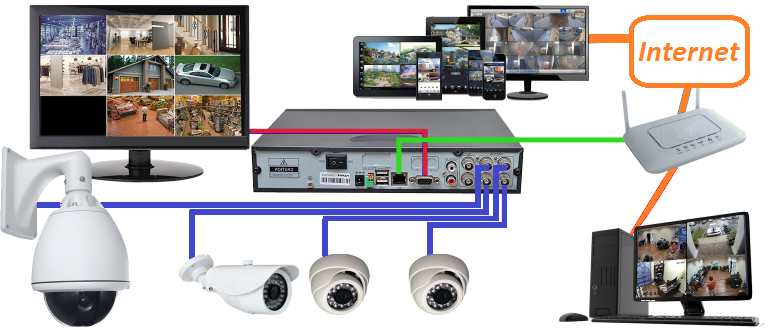
\includegraphics[width=9cm]{img/capitulo_2/sis_videovigilancia.png}
    \end{center}
    \caption{Sistema actual de videovigilancia\\Fuente: Web}
    \label{fig:sistema_video_vigilancia}
\end{figure}

La creciente demanda en el mercado de la vigilancia ha reducido costos en este tipo de sistemas, lo cual permitió que desarrolladores y fabricantes diseñen nuevas implementaciones de sistemas de video vigilancia agregándoles diversas capacidades dependiendo de la tecnología utilizada en su desarrollo. En la figura \ref{fig:surveillance-market} se muestra como el mercado global de la video vigilacia fue avaluado en 42.9 billones de dólares en 2019 y esta proyectado alcanzar a los 69.1 billones billones de dólares hasta el 2026, registrando una taza de crecimiento anual compuesta del 10\% desde el 2020 al 2026. \cite{marketsandmarkets:market-surveillance}\\

\begin{figure}[H]
    \begin{center}
        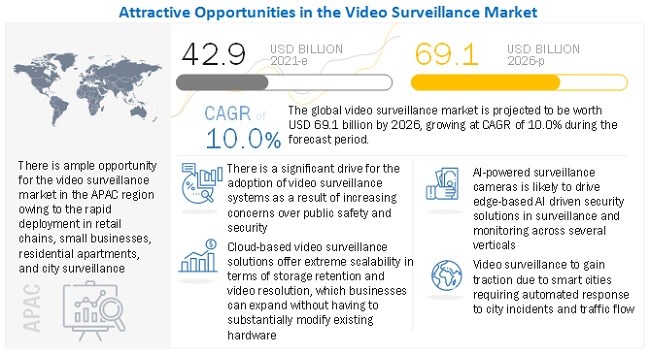
\includegraphics[width=13cm]{img/capitulo_2/surveillance-market.jpg}
    \end{center}
    \caption{Proyección del mercado de la videovigilancia\\Fuente: MarketsAndMarkets(web)}
    \label{fig:surveillance-market}
\end{figure}

El aspecto más importante a resaltar en el mercado de la videovigilancia es la potenciación de funcionalidades de estos sistemas gracias a la Inteligencia Artificial (I.A.) y la escalabilidad por servicios basados en la nube.Las técnicas de la inteligencia de artificial que potencian las utilidades de la videovigilancia son: visión por computadora, redes neuronales convolucionales, Machine Learning, Deep Learning, reconocimiento de patrones. (A completar segun bibliografia)\\

Para el desarrollo del prototipo propuesto se implementan todos los componentes involucrados en el sistema de videovigilancia como ser:
\begin{itemize}
    \item Cámaras (Nodos)
    \item Servidor TCP
    \item Servidor Web
    \item Aplicación Movil (Cliente)
\end{itemize}

A continuación se detalla los componentes que forman parte del prototipo del sistema de video vigilancia inteligente propuesto.

\section{Inteligencia Artificial}
La Inteligencia Artificial (I.A.), es una tecnología innovadora que en los últimos tiempos no esta reservado solo para la investigación sino más bien va tomando parte en el desarrollo de la sociedad. El cerebro es el órgano más increible del cuerpo humano; establece la forma en la que percibimos las imágenes, sonido, olores, sabores y el tacto. Nos permite almacenar recuerdos, experimentar emociones e incluso soñar. Sin él, los seres humanos serían organismos primitivos, incapaces de otra cosa que el más simple de los reflejos. Por lo tanto el cerebro es lo que hace a los seres humanos, seres inteligentes.\\

Durante décadas se ha investigado para construir máquinas inteligentes con cerebros como el del ser humano; asistentes robotizados para limpiar los hogares, coches que se conducen por solos, microscopios que detecten enfermedades automáticamente. Pero en la construcción de estas máquinas artificialmente inteligentes se presentan problemas computacionales complejos; problemas que el cerebro humano puede resolver en una fracción de segundos. Las formas de analizar y resolver este tipo de problemas, es el campo de estudio de la Inteligencia Artificial.

\section{Visión por Computadora}
La visión por computadora es una técnica de recolección de información que surge por la inspiración en el sistema visual humano, el cual es la principal fuente de información para el cerebro. Su meta es de modelar y automatizar el proceso de reconocimiento visual de objetos en la vida real.\\

De los cinco sentidos que poseen las personas, la vista es la más importante. Por lo tanto la visión, es una tarea de procesamiento de información; pero tiene un grado de complejidad elevado, ya que para saber que es lo qué hay en el mundo nuestros cerebros deben ser capaces de representar esta información en toda su abundancia de color, forma, movimiento, detalle y belleza. \cite{iaarbook:artificialvision}\\

Por lo tanto, la visión por computadora o visión artificial compone de un conjunto de herramientas y métodos que permiten obtener, procesar y analizar imágenes del mundo real, con el objetivo de ser tratadas por una computadora. Estos métodos van a permitir automatizar un amplio conjunto de tareas al aportar a las computadoras información que es necesaria para la toma de desiciones en sus tareas asignadas. La visión por computadora trata de imitar a la visión humana, usando geometría y un enfoque estadístico para tratar el problema.\\

\subsection{Aplicaciones}
Esta rama de la Inteligencia Artificial aún sigue en investigación y mejoras donde sus aplicaciones más comunes son:

\begin{itemize}
    \item \textbf{Reconocimiento óptico de caracteres:} Detección automática de símbolos que pertenecen a un alfabeto.
    \item \textbf{Inspección robotizada:} Revisión rápida de piezas para garantizar la calidad de componentes fabricados.
    \item \textbf{Modelado 3D:} Construcción de modelos 3D a partir de fotografías.
    \item \textbf{Imágenes médicas:} Análisis de radiografías.
    \item \textbf{Conducción segura:} Detección de obstáculos por medio de un sistema de conducción asistida por cámaras.
    \item \textbf{Vigilancia:} Monitoreo de intrusos, análisis del tráfico vial, monitoreo de piscinas, etc.
    \item \textbf{Detección de rostros:} Mediante algoritmos de reconocimiento facial se reconocen rostros usados en métodos de biometría.
\end{itemize}

\subsection{OpenCV}
Es una biblioteca de uso libre para el desarrollo de aplicaciones usando visión artificial desarrollada por Intel. Esta libreria reune diversas caracteristicas que la hacen popular, por ejemplo: 
\begin{itemize}
    \item Permite su uso para fines comerciales y de investigación.
    \item Se encuentra disponible par varias plataformas como ser GNU/Linux, Mac OS, Windows y Android.
    \item Documentación completa y explicada, con una comunidad de desarrolladores activa.
\end{itemize}

\begin{figure}[H]
    \begin{center}
        
\includegraphics[width=3cm]{img/capitulo_2/cv2_logo.png}
    \end{center}
    \caption{Logotipo de la libreria\\Fuente: Web}
    \label{fig:cv2_logo}
\end{figure}

Esta biblioteca permite:
\begin{itemize}
    \item El procesamiento de imágenes en su escalado, eliminación de ruido y formateo de imagen y video.
    \item El uso y modificación de sus 2500 modelos pre-optimizados que son incluidos en la libreria, acorde a las necesidades del usuario.
    \item El uso del estado del arte de modelos de visión por computadora como también de aprendizaje de máquina (Machine Learning).
    \item El desarrollo de modelos en varias categorías de investigación como ser: reconocimiento facial, detección y seguimiento de objetos, extracción de modelos 3D, etc.
\end{itemize}

Una de las características mas interesantes de OpenCV es el reconocimiento facial. OpenCV, en su extensa biblioteca de funciones, brinda las capacidades para realizar las tareas de preprocesamiento sin ningún problema, así como los algoritmos de predicción. Además de usar el algoritmo de detección de objetos, es posible usar el seguimiento de objetos, para identificar rostros en una transmisión de video. OpenCV incluso posee funciones para configurar fácilmente el modelo en una transmisión en vivo, como en un video pregrabado \cite{medium:opencv}. 

% \section{Redes Neuronales}

\section{Machine Learning}
Es un subcampo de la inteligencia artificial cuyo objetivo es entender la estructura de la información y ajustar estos datos en modelos que puedan ser entendidos y utilizados por las personas.\\

A diferencia de la computación tradicional, donde los algoritmos son grupos de instrucciones programadas ejecutadas por computadoras para resolver problemas específicos, los algoritmos de Machine Learning entrenan a las computadoras con datos de entrada y usa análisis estadístico para generar valores de salida que caen en un rango específico. Por eso el Machine Learning facilita a las computadoras construir modelos desde datos de ejemplo para automatizar el proceso de toma de decisiones basados en datos de entrada.\\

\subsection{Métodos de Machine Learning}
En el Machine Learning, las tareas son generalmente clasificadas en amplias categorias, las cuales estan basadas en como el aprendizaje es recibido o como la retroalimentación en el aprendizaje esta dado en un sistema desarrollado.\\

Dos de los más ampliamente adoptados de metodos en Machine Learning son el aprendizaje supervisado, que entrena un algoritmo basado en un ejemplo de entrada y salida que esta categorizada por un humano, y el aprendizaje no supervisado, que proporciona el algoritmo sin ningún dato categorizado para permitirle encontrar una estructura dentro de los datos de entrada.\\

\subsubsection{Aprendizaje Supervisado}
En lenguaje supervisado, la computadora esta provista con entradas de ejemplo que estan categorizados con sus salidas esperadas. El proposito de este metodo esta para que el algoritmo pueda "aprender" comparando la actual salida con las ``pensadas'' salidas para encontrar errores y en consecuencia modificar el modelo. El Aprendizaje supervisado por lo tanto usa patrones para predecir valores categorizados en datos no cateogirzados adicionales.\\

Por ejemplo, con aprendizaje supervisado, un algoritmo puede ser alimentado con imagenes de tiburones etiquetados como ``peces'' e imagenes de oceanos etiquetados como agua. Siendo entrenado con estso datos, el algoritmo de aprenizaje supervisado deberia poder despues identificar tiburones sin etiquetar como ``peces'' y oceanos no etiquetados como``agua''.\\

Un uso comun del aprendizaje supervisado es usar datos historicos para predecir estadsiticamente futuros eventos. Se puede usar la informacion historica del stock de un mercado para anticipar futuras fluctuaciones o ser empleado para filtrar correos fraudulentos. En aprendizaje supervisado, fotos de perros etiquetados pueden ser usados como datos de entradas para clasificar fotos de perros no etiquetados.\\

\subsubsection{Aprendizaje No Supervisado}
En el aprendizaje no supervisado, la informacion no esta categorizada, asi que los algoritmos de aprendizaje quedan para encontrar similitudes entre los datos de entrada. Como los datos no etiquetados son mas abundantes que los datos etiquetados. los metodos de ML que facilitan el aprendizaje no supervisado son particularmente valiosos.\\

El objetivo del aprendizaje no supervisado puede ser tan sencillo como descubrir patrones ocultos dentro de set de datos, pero esto puede tambien tener un objetivo de caracteristica de aprendizaje, que permite a la maquina computacional descubrir automaticamente las represetnaciones que son necesarias para clasificar datos en bruto.\\

Aprendizaje no supervisado es comunmente usado para datos transaccionales. Puedes tener un dataset grande de clientes y sus compras, pero como humano probablemente no podras tener sentido de que atributos similares pueden ser dibujados de los perfiles de los clientes y sus tipos de compras. Con esta informacion se alimenta un algoritmo de aprendizaje no supervisado, esto podria determinar que las mujeres de cierto rango de edad quienes compran jabones sin olor estan probablemente embarazadas, and por lo tanto una campania de marketing relacionada con el embarazo y productos para bebé pueden ser etiquetados para esta audiencia con el objetivo de incrementar el numero de compras.\\

\section{Protocolos de red}

\subsection{TCP/IP}

\subsection{HTTP}

\section{Video Streaming}

\subsection{Formatos}

\subsubsection{HLS}

\subsubsection{DASH}

\section{Aplicaciones Móviles}

\subsection{Android}

\subsection{Firebase}

\subsection{Exoplayer}

\section{Python}
Python es un lenguaje de programación interpretado cuya filosofía hace hincapié en la legibilidad de su código. Se trata de un lenguaje multiparadigma, ya que soporta parcialmente la orientación a objetos, programación imperativa y, en menor medida, programación funcional. Es un lenguaje interpretado, dinámico y multiplataforma.\\

Python usa tipado dinámico y conteo de referencias para la administración de memoria. Una característica importante de Python es la resolución dinámica de nombres; es decir, lo que enlaza un método y un nombre de variable durante la ejecución del programa (también llamado enlace dinámico de métodos).\\

\section{Metodología de desarrollo Cascada}
    \chapter{Seguridad en el hogar}

% https://bricoladores.simonelectric.com/seguridad-en-el-hogar-que-debemos-proteger

% https://bricoladores.simonelectric.com/medidas-generales-basicas-de-seguridad-en-el-hogar

\section{Introducción}
La seguridad en el hogar es un tema relevante y delicado de manejar, principalmente cuando se trata del espacio vital más importante de todos, donde convive el ser humano. En el hogar se establecen los vínculos más íntimos y personales; entonces la seguridad en el hogar es un factor de gran importancia. La mayoría de percances como intrusión de un extraño, allanamientos y robos se producen durante su ausencia. Los motivos son varios: desde un viaje prolongado a salidas puntuales, regulares y/o diarias. Una vivienda vacía es más vulnerable que otra ocupada y este aspecto se toma en cuenta en el diseño de un sistema de seguridad para el hogar, el cual debe ofrecer características que ayuden a minimizar el impacto de las situaciones de peligro.\\

\section{Ausencia en el hogar}
En materia de seguridad del hogar, cualquier precaución, resulta de utilidad para prevenir, que ocurran incidentes y mantener protegidos a los seres más cercanos. De hecho el objetivo de la seguridad implica la toma de precauciones necesarias para que un lugar sea seguro para las personas. Incluso las personas más retraídas y amantes de la soledad y el aislamiento deben, en un momento u otro, salir de su residencia habitual, algo que se convierte en largas horas de ausencia en la mayoría de los casos (evidentemente por trabajo, obligaciones académicas y otros menesteres cotidianos), y ocasionalmente, con mayor o menor asiduidad, por otras razones menos frecuentes (viajes, vacaciones, etc).\\
 
Todas las posibles situaciones a presentarse se definen en función del tiempo de ausencia; de modo que se establecen distintos casos con aspectos peculiares y específicos referentes a la seguridad y los riesgos; por ejemplo exponer las medidas de protección más básicas y elementales que siempre deben tomarse en cuenta, como el contrato de un seguro para la vivienda (con elementos importantes que figuran en toda póliza para su elección y contratación).\\

Un seguro contra robos puede proteger de alguna manera los daños materiales que pueden ocurrir, pero incluso para probar la veracidad del suceso es necesario presentar pruebas visuales que sirvan de referencia en la denuncia. Una imágen como en la figura \ref{fig:intruso} puede ayudar incluso en una investigación.\\

\begin{figure}[H]
    \begin{center}
        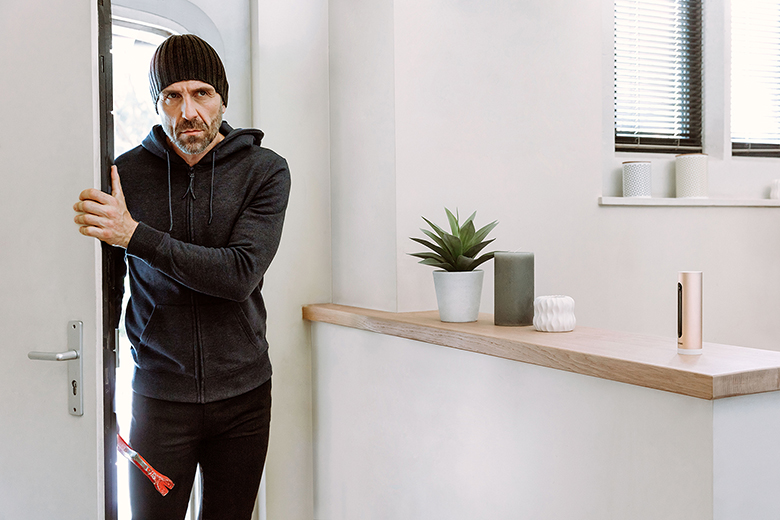
\includegraphics[width=7cm]{img/capitulo_3/intruso.jpg}
    \end{center}
    \begin{center}
        \caption{Ilustración de ejemplo de un intruso.}
        Fuente: Web
        \label{fig:intruso}
    \end{center}
\end{figure}

A continuación se detallan las situaciones más comunes que pueden presentarse, con sus respectivas acciones sugeridas para disminuir el peligro.\\

\subsection{Ausencias cotidianas}
Las ausencias diarias de horas o minutos son las más comunes y brindan oportunidades a asaltantes atentos. Para este caso se puede tener en cuenta medidas de protección sencillas y sin complicaciones que cualquiera puede llevar a cabo sin inversión alguna. Asegurar los cierres de los accesos a la vivienda, disimular las ausencias o evitar proporcionar información sobre nuestros hábitos, son algunas de las medidas que se exponen para evitar intrusiones no deseadas en el hogar.\\
 
% Como situación perteneciente a este grupo de supuestos, pero con riesgos añadidos y particularidades propias que obligan a prestarle una atención especial, se tratará aparte el caso de ausencias puntuales dejando en la vivienda a niños, personas mayores o dependientes sin nadie a su cargo. Evidentemente, aquí se tratarán amenazas y riesgos internos de la vivienda, tales como manipulaciones indebidas de instalaciones y componentes de especial peligrosidad, o la atención a emergencias que puedan suceder durante ausencias breves.\\

\subsection{Ausencias de termino medio}
Cuando uno sale de casa previamente sabe si uno va ha volver al cabo de pocas horas, de unos días o de semanas; en cada caso se pueden presentar algunas peculiaridades y riesgos específicos que se deben afrontar de distintos modos. En este supuesto, tras las ausencias cotidianas, se detallan los casos de ausencias de pocos días, especialmente en fines de semana, puentes festivos y vacaciones cortas. En estas situaciones convergen la necesidad de contar con alarmas y avisadores técnicos, con la de disponer de sistemas de alarma y dispositivos antiintrusión los cuales, como veremos, pueden ser de muy diversa índole.\\

\subsection{Ausencias prolongadas}
Las vacaciones y las estancias de cierta duración en lugares alejados de nuestras residencias habituales ofrecen oportunidades únicas a posibles asaltantes. No ofrecer información sobre nuestro paradero, tratar de evitar el efecto de vivienda vacía, contar con la supervisión regular de alguien de confianza en nuestra ausencia y mantener a buen recaudo bienes u objetos de valor serán, en estos casos, las principales prioridades (sobre todo en el caso de las segundas residencias, una cuestión que también consideraremos detalladamente como caso diferenciado).\\

\section{Situaciones de riesgo}
\subsection{Presencia de instrusos}
Un intruso o persona ajena siempre representa un peligro en el interior de nuestro hogar y aún más cuando se desconoce el motivo de su presencia. La posibilidad de robos en cualquier cuidad del mundo esta presente y aun mas cuando este entra al interior de un hogar forzando cerraduras, encapuchado, especialmente cuando los habitantes de la casa no estan. En la figura \ref{fig:ladron}, se muestra una ilustracion de ejemplo de un intruso forzando la puerta de una casa.\\

\begin{figure}[H]
    \begin{center}
        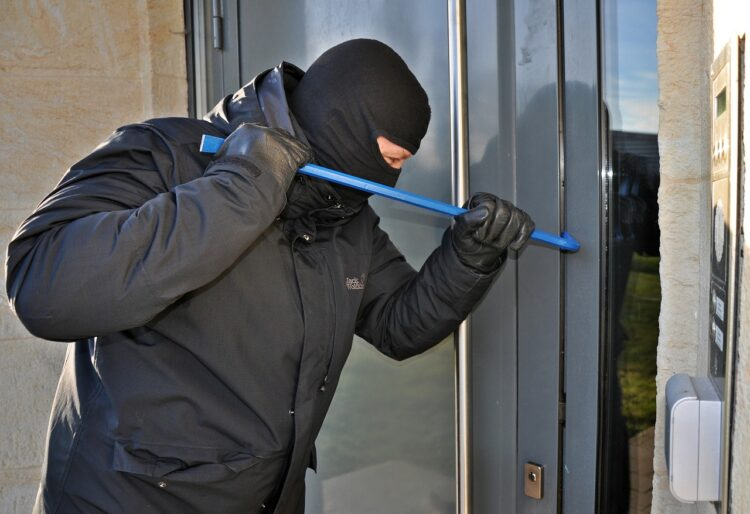
\includegraphics[width=5cm]{img/capitulo_3/burglar.jpg}
    \end{center}
    \begin{center}
        \caption{Ilustración de ejemplo de un ladrón.} 
        Fuente: Web
        \label{fig:ladron}
    \end{center}
\end{figure}

\subsection{Fuego y humo}
El fuego es una reacción quimica, donde un conjunto de partículas o moléculas incandecentes en materia combustible es capaz de emitir calor y luz. Con el calor se pueden llegar a desintegrar muchos objetos y estos mismos servir de combustion para que el fuego se expanda.
Este fenómeno es uno de los principales causantes de tragedias en la actualidad, tanto como incendios forestales y/o colectivos, incendios en interiores, como ser: casas, departamentos o sitios cerrados. En la figura \ref{fig:fuego} se visualiza la facilidad con la que el fuego puede expandirse en interiores.\\

\begin{figure}[H]
    \begin{center}
        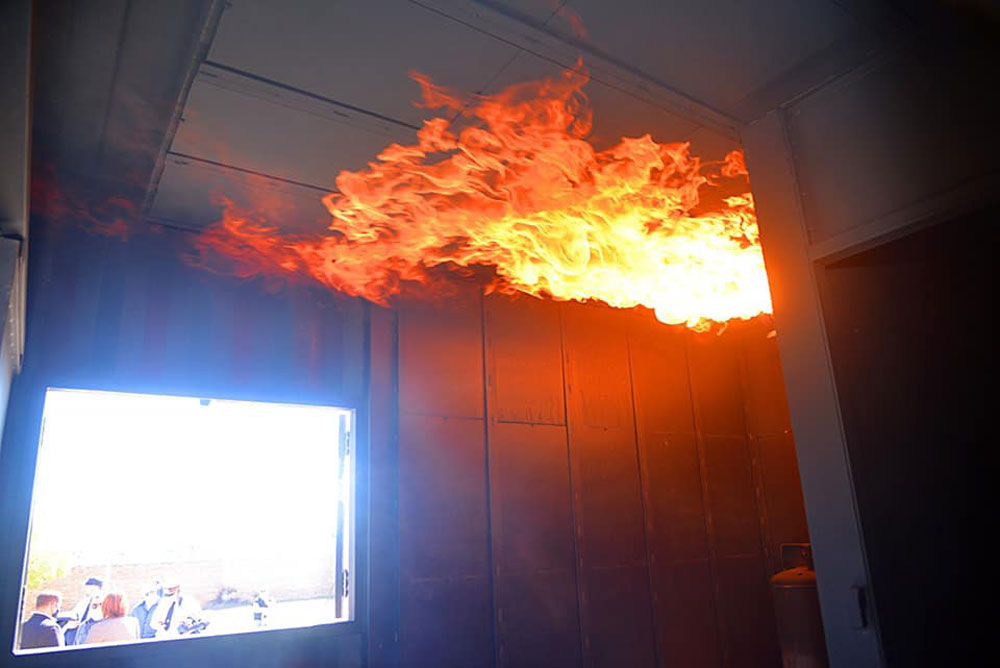
\includegraphics[width=5cm]{img/capitulo_3/fuego_en_interiores.jpg}
    \end{center}
    \begin{center}
        \caption{Ilustración decenas ejemplo de fuego en interiores.} 
        Fuente: Web 
        \label{fig:fuego}
    \end{center}
\end{figure}

El humo acompañado del fuego son elementos muy perjudiciales tanto como a las personas como al medio ambiente en general. El humo es uno de los factores principales que afectan a la salud respiratoria de las personas y animales. Identificar a tiempo la presencia de humo puede incluso prevenir y/o predecir la organización de fuego  evitar tragedias.\\

En la figura \ref{fig:humo}, se visualiza como la presencia de humo puede ayduar a alertar de que hay fuego en el interior de una casa o habitación.\\

\begin{figure}[H]
    \begin{center}
        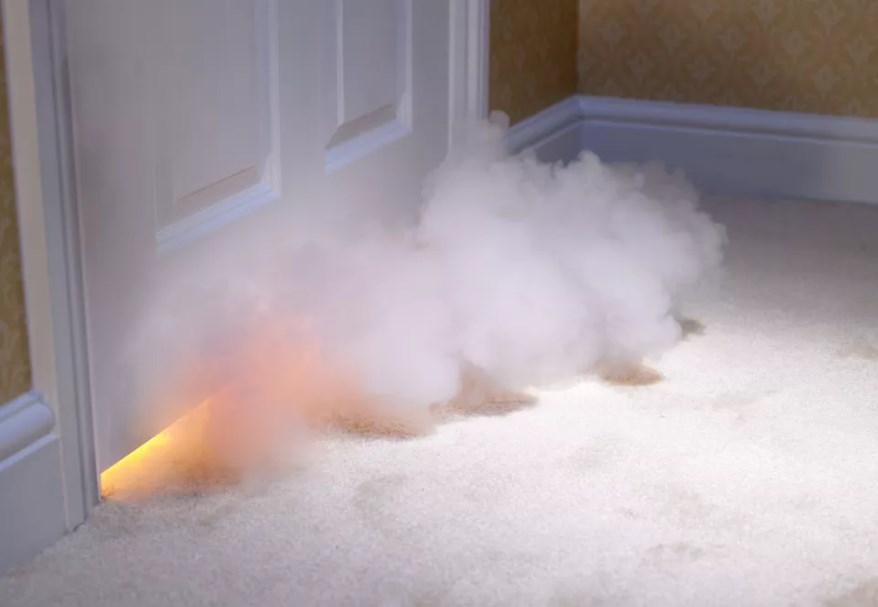
\includegraphics[width=5cm]{img/capitulo_3/fuego_en_el_cuarto.jpg}
    \end{center}
    \begin{center}
        \caption{Ilustración de la presencia de fuego y humo en una habitación cerrada.}
        Fuente: Web.
        \label{fig:humo}
    \end{center}
\end{figure}

\section{Sistemas de seguridad}
En el mercado, existe una gran variedad de artefactos, que están al alcance de todos para proteger los hogares frente a cualquier tipo de amenaza, tanto interna como externa. Los más eficaces y eficientes, son los sistemas electrónicos de seguridad. No obstante, sea cual sea la opción elegida se debe tener en cuenta los siguientes riesgos y amenazas:\\

\begin{itemize}
    \item \textbf{Allanamientos, intrusiones y vandalismo:} riesgos procedentes del exterior, que se pueden mitigar fácilmente instalando cierres de alta seguridad en los accesos a la vivienda, alarmas anti-intrusión u otros mecanismos disuasorios.
    \item \textbf{Accidentes domésticos:} riesgos procedentes del interior de hogar que pueden poner en riesgo la integridad física y/o moral de sus habitantes, tanto personas como mascotas, así como los bienes que contienen e incluso la misma infraestructura.
\end{itemize}

Las alarmas técnicas (alertas de fugas y escapes) y de emergencia son los sistemas más adecuados para proteger una vivienda. También es preciso tomar las medidas oportunas para proteger los componentes más sensibles del hogar (instalaciones de suministros y otros elementos de riesgo) de manipulaciones indebidas, golpes y otro tipo de percances que pueden ocasionar accidentes o situaciones indeseables.\\

\subsection{Alarmas}

Las alarmas son artefactos sonoros que emiten un sonido que provoca la alerta en las personas. Existen de diferentes tipos, medidas y campo de uso. El volúmen y el sonido es claramente diferenciado de cualquier objeto que emita un sonido cualquiera. Este objeto es utilizado generalmente para poner en alerta a todas las personas que lleguen a escucharlo y/o comunicar peligro.
En la figura \ref{fig:bocinas} se puede apreciar un modelo particular de alarmas sonoras.

\begin{figure}[H]
    \begin{center}
        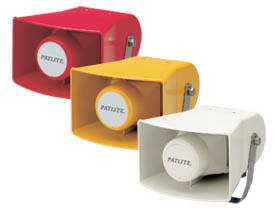
\includegraphics[width=3cm]{img/capitulo_3/alarmas.jpg}
    \end{center}
    \begin{center}
        \caption{Ilustración de alarmas con sonido.}
        Fuente: Web.
        \label{fig:bocinas}
    \end{center}
\end{figure}

\subsection{Sensores}
Los sensores son dispositivos que captan magnitudes físicas (variaciones de luz, temperatura, sonido, etc.) u otras alteraciones de su entorno. Los detectores de humo son dispositivos desarrollados para detectar la presencia de un incendio en el interior de un edificio. En la figura \ref{fig:detector_humo} se aprecia un modelo en particular de sensor de detección de humo.\\

\begin{figure}[H]
    \begin{center}
        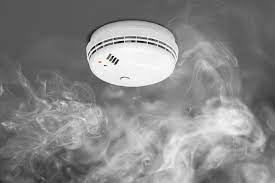
\includegraphics[width=5cm]{img/capitulo_3/sensor_de_humo.jpg}
    \end{center}
    \begin{center}
        \caption{Ilustración de detector de humo.}
        Fuente: Web.
        \label{fig:detector_humo}
    \end{center}
\end{figure}

\subsection{Cámaras}

Las cámaras son dispositivos que permiten registrar imágenes estáticas y en movimiento. Específicamente las cámaras de vigilancia son las que se encargan de grabar todo lo que puede ocurrir en una casa o negocio. Contar con este tipo de cámara puede proporcionar sensación de seguridad y protección. Disponer de este tipo de sistemas puede resultar ser una solución para mantenerse protegido. El desarrollo de la tecnología ha logrado que el sector de la seguridad disponga de equipos eficientes y con diversas funcionalidades. En la figura \ref{fig:camaras} se visualizan diferentes modelos de cámaras de seguridad que se encuentran en el mercado.\\

\begin{figure}[H]
    \begin{center}
        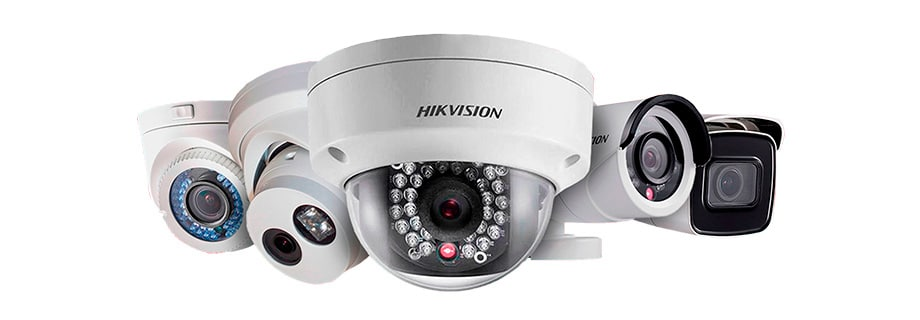
\includegraphics[width=6cm]{img/capitulo_3/camaras.jpg}
    \end{center}
    \begin{center}
        \caption{Ilustración de diversas cámaras de seguridad.}
        Fuente: Web.
        \label{fig:camaras}
    \end{center}
\end{figure}

El tipo más común en el mercado son las cámaras de interiores ya que son las más sencillas y económicas del mercado ya que no necesitan mucho mecanismo ni protección. En la figura \ref{fig:camara} se visualiza un ejemplo de cámara de interiores.\\

\begin{figure}[H]
    \begin{center}
        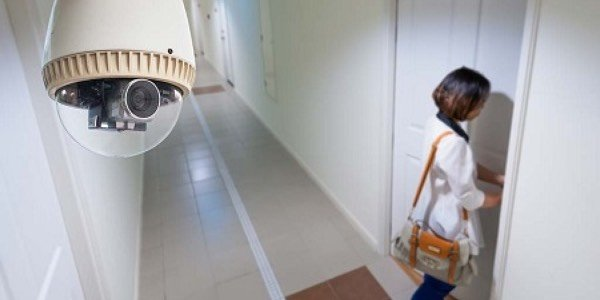
\includegraphics[width=5cm]{img/capitulo_3/camara_de_interiores.jpg}
    \end{center}
    \begin{center}
        \caption{Cámara de vigilancia de interiores.}
        Fuente: Web.
        \label{fig:camara}
    \end{center}
\end{figure}

Seguridad y vigilancia son aspectos que se requieren en todo el mundo; gobiernos, empresas, instituciones financieras, organizaciones de salud, necesitan cierto grado de medidas de seguridad y como resultado se generó un dramático incremento en la demanda de aplicaciones de seguridad como por ejemplo video vigilancia, monitoreo y grabación de: fronteras, puertos, transporte, hogares, corporaciones, instituciones educativas, lugares públicos, edificios, etc.\\

% Sistemas de videovigilancia inteligente La técnica clave del reconocimiento de la accion humana basada en la vision  por compoutadora consiste en describir y comprender los comportamientos humanos por medio de la vision por computadora.\\

% Este proceso es una tarea complicada e integra algunos campos de investigacion que incluyen el procesamiento de imagen, aperndizaje automatico, reconocimiento de patrones, etc.\\

% La detección de un objeto móvil consiste en separar las áreas de cambio en el video es decir en las imádgenes de fondo que comprenden el video, dicho de otra manera, separar correctamente las áreas y contornos del objetico movil. Es critico para el siguiente procesamiento la segementación efectiva \\

    \chapter{Análisis y Diseño}

En las etapas iniciales de la metodología ``Cascada'', se realiza el análisis del problema y diseño previo del sistema, todo esto al inicio de la implementación del producto final. Es importante que estas fases sean completadas en su totalidad para que el desarrollo sea exitoso. Este proyecto plantea el diseñado y desarrollo para 70 dias hábiles según calendario, con la distribución del tiempo definido según la complejidad de las tareas que implican cada una de las fases.\\

\section{Análisis}
Para el diseño del Sistema de video-vigilancia inteligente, es necesario tener en cuenta los elementos principales que lo componen. Un sistema de video-vigilancia esta compuesto de cámaras individuales y un puesto central o servidor donde todas las conexiones convergen y su control es centralizado. En el dispositivo central (servidor) se procesan las imágenes que las cámaras capturan y se convierten en video para ser visualizado en un monitor.\\

El sistema propuesto permite visualizar video en vivo desde cualquier dispositivo con acceso a la red de internet además de que envía notificaciones automáticas en el instante en que se detecta: movimiento, fuego, o silueta de un intruso. El usuario recibe la notificación por correo electrónico el cual adjunta capturas y un enlace web para visualizar en vivo lo que esta captando la cámara.\\

% Los principales módulos del sistema son:
% \begin{itemize}
%     \item Módulo de cámara (Nodos)
%     \item Módulo de servidor (Analizador y noti)
%     % \item Servidor HTTP (Servicio que aplica el protocolo de la Web)
%     % \item Módulo SMTP (Módulo de envio de correo electrónico)
% \end{itemize}

En la figura \ref{fig:system_desing} se visualiza el esquema general del sistema propuesto. Las cámaras de video-vigilancia se encargan de capturar los fotogramas de video y se enlazan por medio de un socket o conector (uno por cada cámara) al servidor central. Cuando es registrada una nueva conexión, el sistema notifica al usuario por medio de un correo electrónico, compartiendo información relevante sobre la conexión de una nueva cámara. El servidor central, maneja todas las conexiones, además realiza el análisis de los fotogramas de manera individual por cada cámara conectada por medio de una libreria de visión por computadora. De forma paralela se construye el video que se va a transmitir a partir de los fotogramas, siendo decodificado por medio de un conjunto de paquetes de software libre, los cuales arman las partes del archivo para el streaming de video por medio de la red. Cuando un evento (fuego, movimiento, silueta humana) es identificado, automáticamente el sistema envia la notificación correspondiente por medio de correo electronico al usuario avisando una posible situación identificada.\\

\begin{figure}[H]
    \begin{center}
        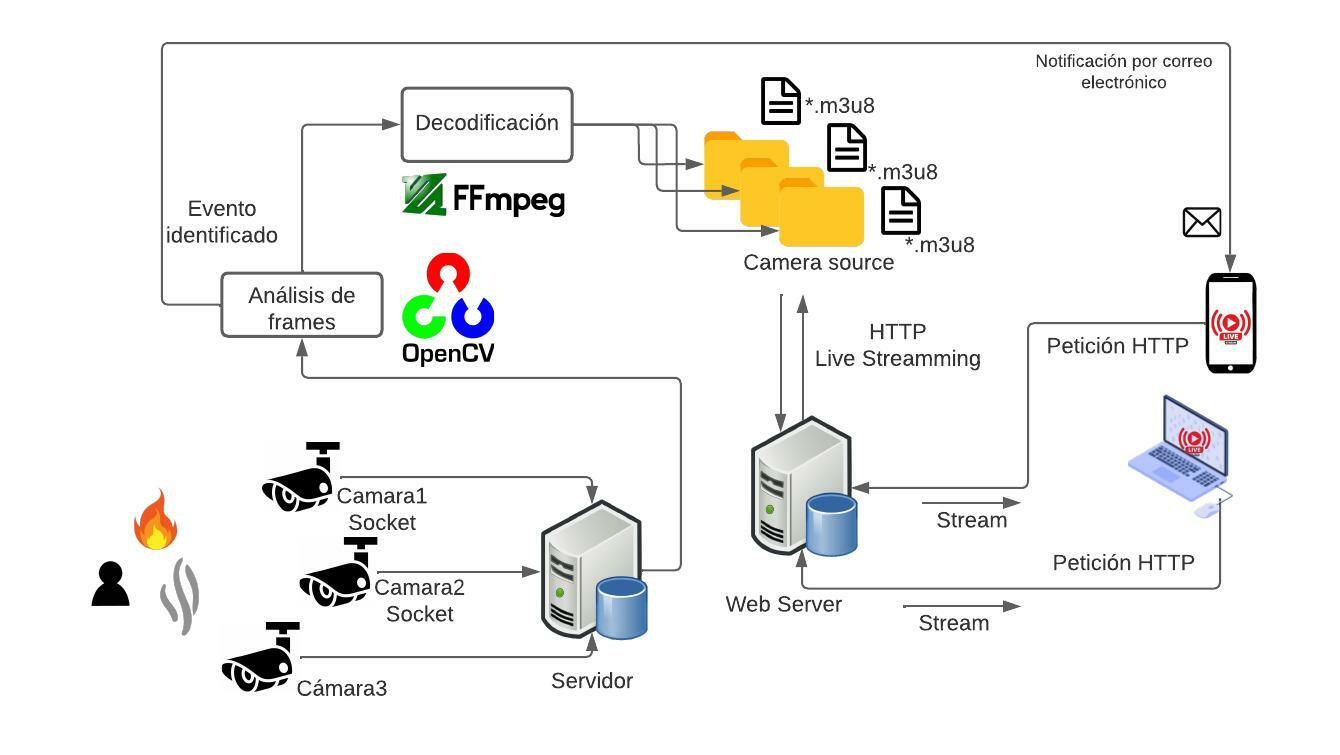
\includegraphics[width=17cm]{img/capitulo_4/main.jpeg}
        \caption{Diseño de interacción de los módulos del sistema de video-vigilancia.}
        Fuente : Elaboración propia.
        \label{fig:system_desing}
    \end{center}
\end{figure}

\subsection{Definición de Requerimientos}
La definición de requerimientos es una de las actividades más importantes del desarrollo de software; de ello depende el resto de actividades del proyecto. Anteriormente se describe completamente el comportamiento del sistema que se desarrolla para la identificación de los requerimientos. Inicialmente se plantean los criterios de partida a tomar en cuenta en el diseño del sistema de video-vigilancia inteligente:

\begin{enumerate}
    \item Costos altos en la infraestructura de transmisión de video en vivo.
    \item Las características de identificación automática, estan disponibles para sistemas de video-vigilancia de alto nivel.
    \item Una alerta inmediata puede minimizar el impacto de alguna situación que ponga en peligro la integridad de bienes materiales y humanos.
    \item Los usuarios finales son personas que a menudo dejan su hogar para salir a trabajar, y usan constamente su correo electrónico.
\end{enumerate}

A partir de estos criterios planteados a continuación se definen los requerimientos funcionales y no funcionales:

\begin{itemize}
    \item \textbf{Requerimientos Funcionales}
    En esta fase es necesario delimitar el alcance y las capacidades del sistema planteado para la realización de la planificación inicial, estimación de tiempos, diseño y desarrollo. Para ello se define la lista de requerimientos funcionales del sistema de video-vigilancia inteligente.
    
    \begin{table}[H]
        \caption{Lista de requerimientos funcionales }
        \label{tabla:req_funcionales}
        \begin{center}
            \begin{tabular}{ |c|l|} 
                \hline
                1. & Capturar fotogramas por medio de una o varias cámaras portatiles.\\ \hline
                2. & Visualizar fotogramas capturados en tiempo real (captura de video).\\  \hline
                3. & Notificar al usuario cuando una nueva cámara se conecta.\\  \hline
                4. & Notificar al usuario cuando una cámara se desconecta.\\  \hline
                5. & Enviar fotogramas capturados por medio de la red al servicio encargado de su análisis.\\ \hline
                6. & Análizar y procesar fotogramas capturados individualmente por cada cámara.\\  \hline
                7. & Permitir la recepción de fotogramas de varias fuentes hacia el servicio.\\ \hline
                8. & Transmitir los fotogramas convertidos en video en vivo desde fuentes diferentes.\\ \hline
                9. & Detectar movimiento a partir de fotogramas recibidos desde distintas fuentes.\\ \hline
                10. & Detectar silueta humana a partir de fotogramas recibidos desde distintas fuentes.\\ \hline
                11. & Detectar fuego a partir de fotogramas recibidos desde distintas fuentes.\\ \hline
                12. & Notificar al usuario por medio de un correo electrónico cuando se de una detección.\\ \hline
            \end{tabular}
        \end{center}
        \begin{center}
            Fuente: Elaboración propia.
        \end{center}
    \end{table}

    \item \textbf{Requerimientos No Funcionales}
    Los requerimientos no funcionales son aquellos relacionados con la calidad y el proceso de desarrollo del sistema. Los tipos de requisitos no funcionales aplican: rendimiento, disponibilidad, accesibilidad, usabilidad, estabilidad, portabilidad, costo, operatividad, interoperabilidad, escalabilidad, concurrencia, mantenibilidad, interfaz, plazo de entrega y herramientas. Los requisitos no funcionales surgen de la necesidad del usuario, debido a las restricciones en el presupuesto y las herramientas utilizadas.\\
    
    \begin{enumerate}
        \item  \textbf{Requisitos de interfaz} 
            \begin{itemize}
                \item Las cámaras tendran una interfaz que permita visualizar la tarea que ejecutan.
                \item El servidor mostrará información necesaria sobre las tareas que realiza.
                \item El sistema deberá ser de fácil configuración.
                \item Las notificaciones por correo electrónico deberán ser visualmente estilizadas.
            \end{itemize}
        \item \textbf{Requisitos de portabilidad}
            \begin{itemize}
                \item Los módulos de cámara podran conectarse de forma cableada o inalámbrica.
            \end{itemize}
        \item \textbf{Requisitos de disponibilidad}
            \begin{itemize}
                \item La transmisión en vivo estará disponible cuando el usuario quiera visualizar lo que captan las cámaras.
            \end{itemize}
    \end{enumerate}

\end{itemize}

\section{Planificación}
Todas las fases del modelo cascada son planificadas según la complejidad y tareas que presenta cada fase. Dado que cada fase debe culminarse por completo para pasar a la siguiente o en su defecto requerir mínimas modificaciones para regresar a la fase anterior, se plantea una planificación de 70 días hábiles que se visualiza en la tabla \ref{tabla:planning}.\\

\begin{table}[H]
    \caption{Tabla de planificación según fases del modelo Cascada.}
    \label{tabla:planning}    
    \begin{center}
        \begin{tabular}{|c|l|c|c|c|}
            \hline
            \textbf{Num.} & \textbf{Fase del modelo Cascada}  &  \textbf{Fecha inicial} & \textbf{Fecha final} & \textbf{Duración (días)}\\ \hline
            \textbf{1.} & Fase de análisis        & 6-jun        & 17-jun        & 10        \\ \hline
            \textbf{2.} & Fase de diseño del sistema       & 20-jun        & 8-jul        & 15        \\ \hline
            \textbf{3.} & Fase de implementación        & 11-jul        & 19-ago        & 30        \\ \hline
            \textbf{4.} & Fase de pruebas        & 22-ago         &   2-sep     &    10     \\ \hline
            \textbf{5.} & Fase de mantenimiento        & 5-sep        & 9-sep        & 5        \\ \hline
        \end{tabular}
    \end{center}
    \begin{center}
        Fuente: Elaboración propia.
    \end{center}
\end{table}

En la figura \ref{fig:gannt} se visualiza e diagrama de Gannt en base a la planificación expresada en la anterior tabla.
\begin{figure}[H]
    \begin{center}
        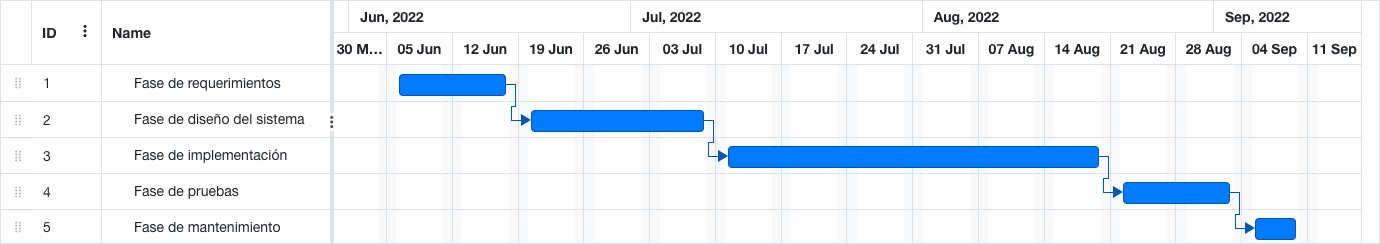
\includegraphics[width=18cm]{img/capitulo_4/gant.png}
    \end{center}
    \begin{center}
        \caption{Diagrama de Gannt.}
        Fuente : Elaboración propia.
        \label{fig:gannt}
    \end{center}
\end{figure}

% \section{Diseño}
% El diseño del sistema de video-vigilancia se divide y se desarrolla según los módulos que componen el sistema completo:
% \begin{itemize}
%     \item Módulo de cámaras
%     \item Módulo de servidor
% \end{itemize}

\section{Diseño del módulo de cámaras}
El módulo de cámaras permite el control de conexión de una cámara al servidor central. Permite conectar una cámara web o una cámara de  una Raspberry Pi. Presenta campos para ingresar datos de configuración que permiten la conexión al servidor central.\\

\subsection{Diseño de interfaz}
En la figura \ref{fig:cam_user_interface} se presenta el esbozo de interfaz de ususario que servirá de diseño final para el desarrollo del presente módulo. El módulo de cámaras permite la visualizacion de fotogramas capturados por medio de la cámara conectada, configuración de la conexión y verificación del estado de envio de los fotogramas al servidor.

\begin{figure}[H]
    \begin{center}
        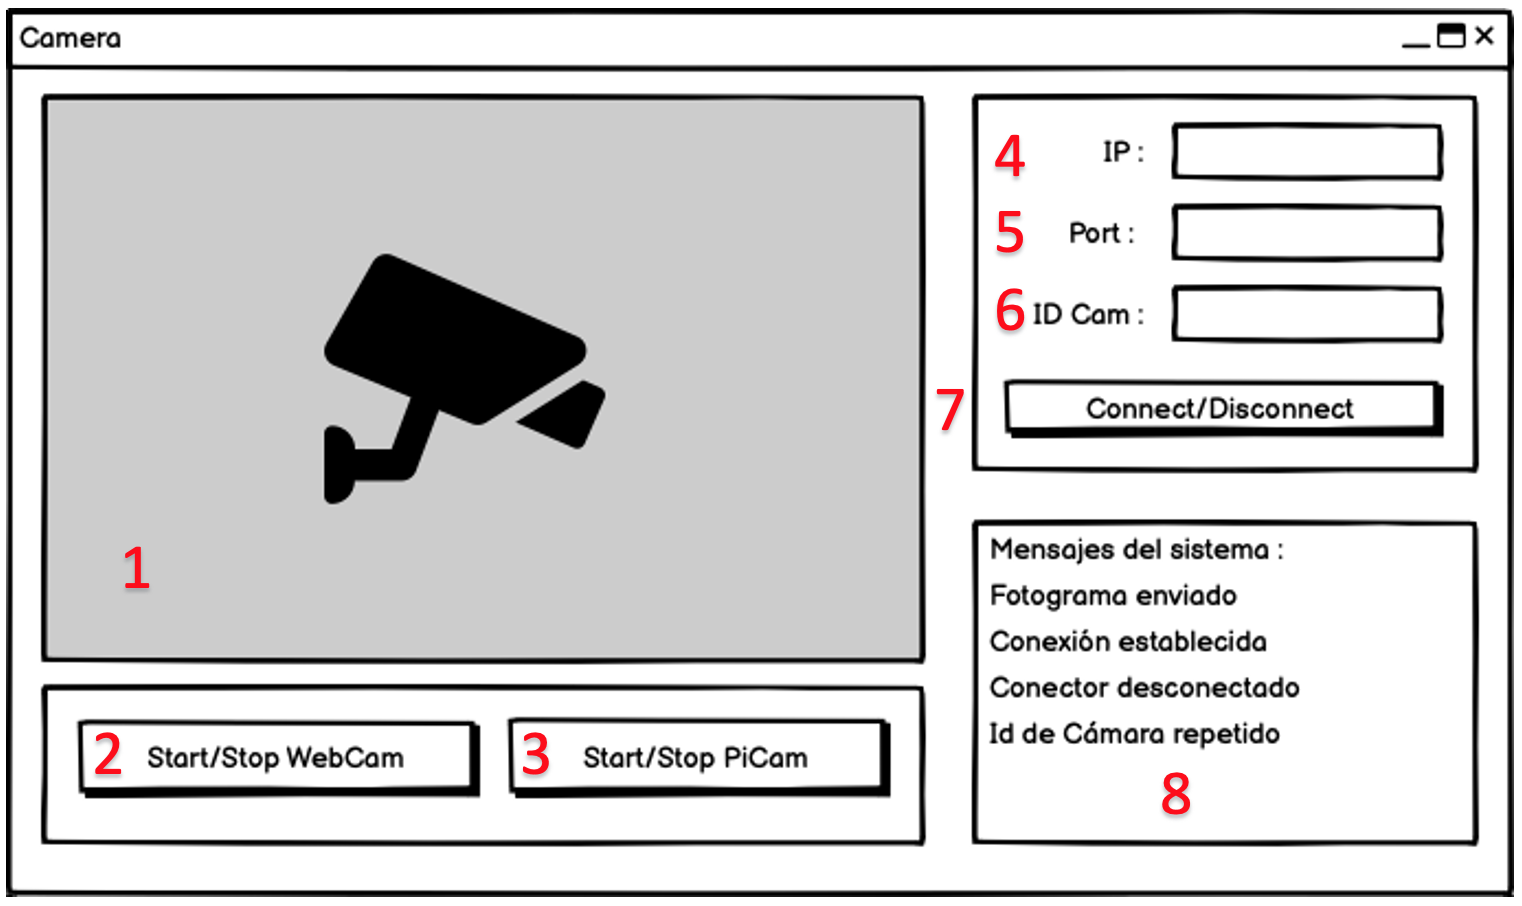
\includegraphics[width=13cm]{img/capitulo_4/camera_interface.png}
    \end{center}
    \begin{center}
        \caption{Diseño de interfaz gráfica de usuario (Módulo de cámaras).}
        Fuente: Elaboración propia.
        \label{fig:cam_user_interface}
    \end{center}
\end{figure}

A continuación se describe a detalle cada uno de los elementos que conforman la interfaz de usuario del módulo de cámaras.
\begin{enumerate}
    \item \textbf{Pantalla}: Espacio de  visualización de los fotogramas que capta la cámara conectada.
    \item \textbf{Botón WebCam}: Botón de conexión/desconexión para la cámara web
    \item \textbf{Botón PiCam}: Botón de conexión/desconexión para la cámara de Raspberry Pi.
    \item \textbf{Campo de dirección IP}: Campo de texto para que el usuario ingrese la dirección IP del servidor.
    \item \textbf{Campo de número de puerto}: Campo de texto para que el usuario ingrese el puerto de escucha del servidor.
    \item \textbf{Campo de identificador de la cámara}: Campo de texto para que el usuario ingrese el número identificador de la cámara conectada.
    \item \textbf{Botón de conexión}: Botón de conexión/desconexión al servidor para el envio de fotogramas al servidor.
    \item \textbf{Cuadro de mensajes}: Cuadro de lista para mostrar diferentes mensajes de módulo: envio de fotogramas, conexión/desconexión al servidor, etc.
\end{enumerate}

\subsection{Diagrama de secuencia}
En la figura \ref{fig:diag_sec_mod_camera} se ilustra el diagrama de secuencia del módulo de cámaras. El diagrama describe de forma gráfica el comportamiento de la interacción entre el módulo de cámaras con el servidor.

\begin{figure}[H]
    \begin{center}
        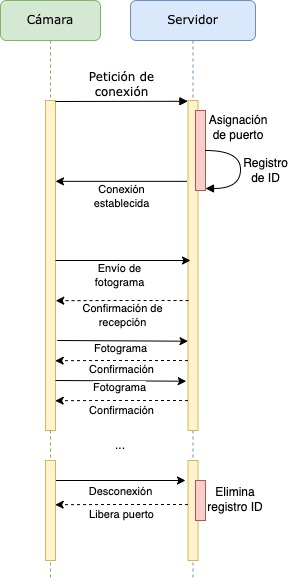
\includegraphics[width=7cm]{img/capitulo_4/sec_cam_serv.jpg}
    \end{center}
    \begin{center}
        \caption{Diagrama de interacción entre el módulo de cámaras con el servidor.}
        Fuente: Elaboración propia.
        \label{fig:diag_sec_mod_camera}
    \end{center}
\end{figure}

La interacción entre el módulo cámaras y el servidor es como sigue:
\begin{enumerate}
    \item El módulo de cámaras realiza una petición de conexión al servidor.
    \item El servidor acepta la petición y le asigna un puerto de escucha a esa nueva conexión.
    \item Se registra el identificador de la cámara para evitar duplicidad en los identificadores.
    \item El servidor envia un mensaje de confirmación de conexión.
    \item El módulo de cámaras envia un fotograma.
    \item El servidor confirma la recepción del fotograma.
    \item Se repiten los anteriores pasos mientras dura la conexión.
    \item El módulo de cámaras se desconecta del conector asignado.
    \item El servidor elimina el registro del identificador de la cámara y libera la conexión. 
\end{enumerate}

% \subsubsection{Diagrama de estado}
% Se estudia los casos en los que el usuario interactura con el módulo de cámara.
% \begin{itemize}
%     \item Usuario inicializa la cámara
%     \item Ingresa la configuracion
%     \item Si hay un dispositivo con la misma configuracion se recahza la conexión.
%     \item sigue el proceso exitoso.
% \end{itemize}
\subsection{Diagrama de clases}
De acuerdo al planteamiento de comportamiento del módulo de cámaras, para el desarrollo de este módulo se plantea el diagrama de clases que se visualiza en la figura \ref{fig:camera_clases}.\\

\begin{figure}[H]
    \begin{center}
        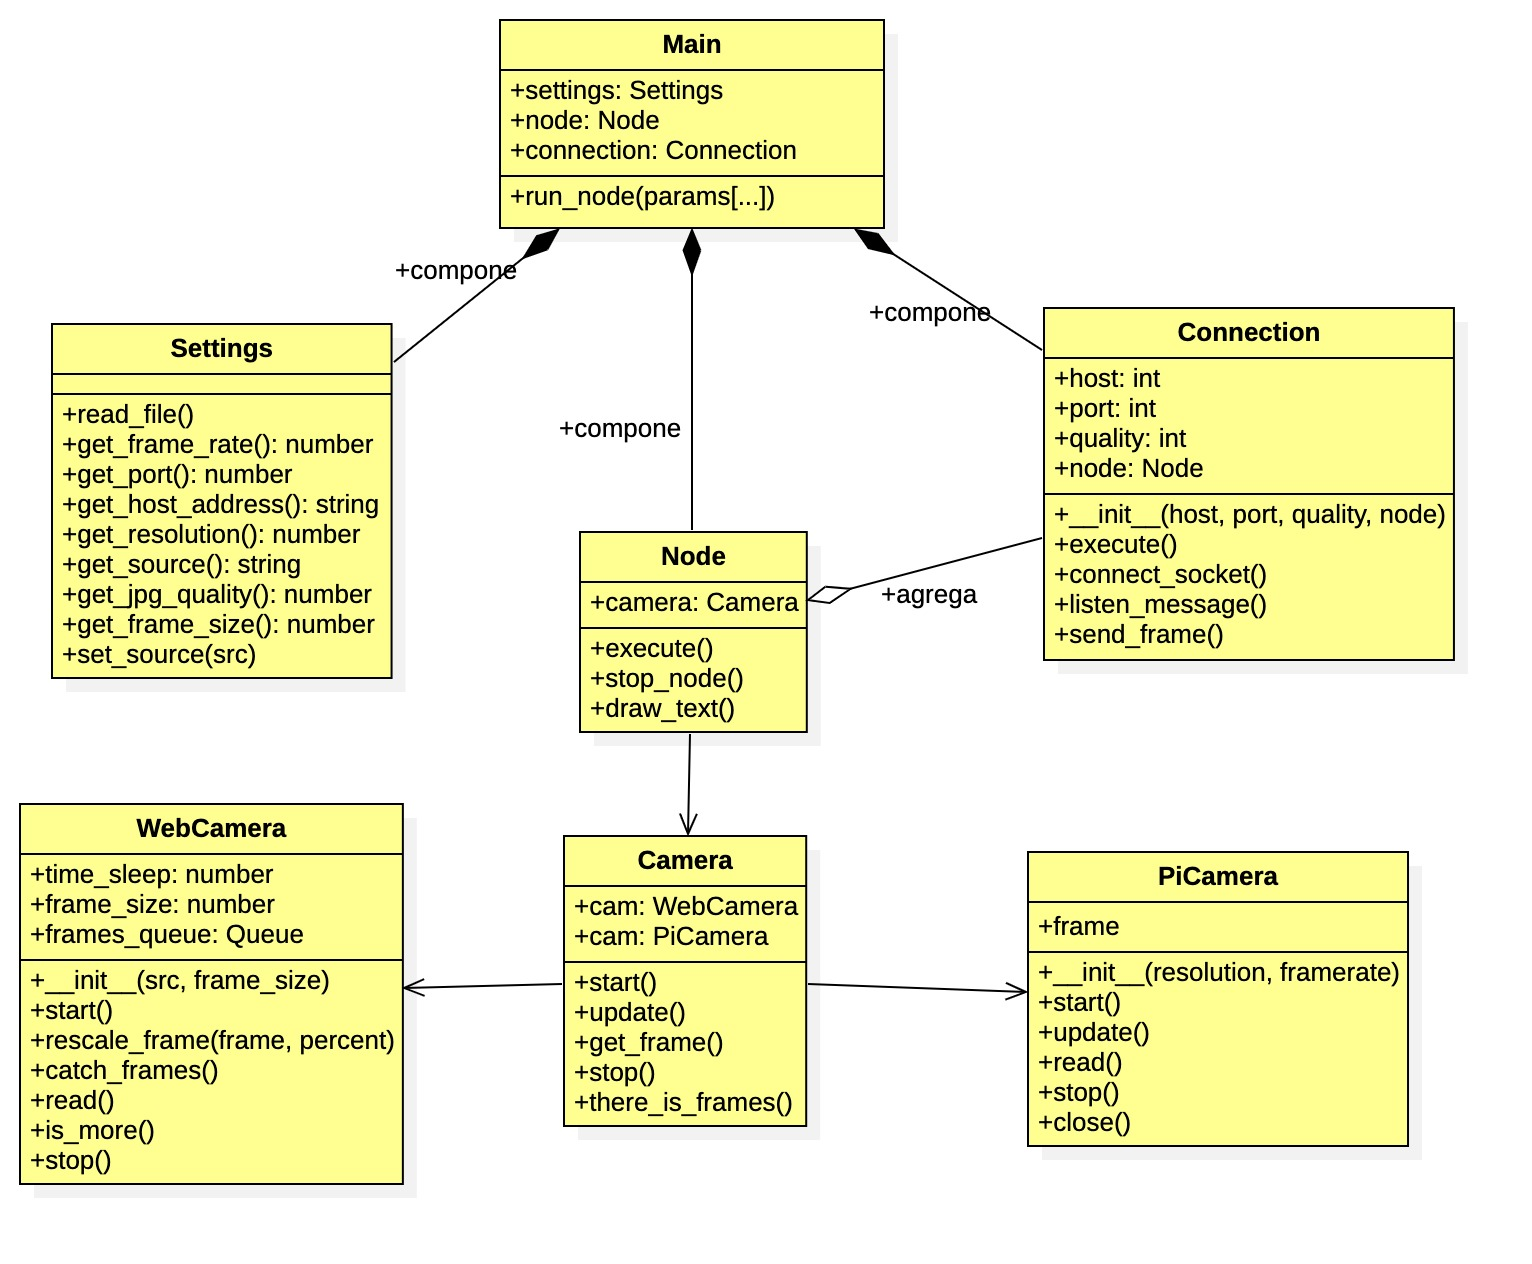
\includegraphics[width=15cm]{img/capitulo_4/camera_clases.jpg}
        \caption{Diagrama de clases del módulo de cámaras.}
        Fuente : Elaboración propia.
        \label{fig:camera_clases}
    \end{center}
\end{figure}

Para la comprensión de este diagrama de clases se procede a describir cada clase con sus respectivos atributos y métodos.\\

\begin{itemize}
    \item \textbf{Main}: Clase principal encargada de inicializar las instancias necesarias para el módulo de cámaras. Sus atributos son:
        \begin{itemize}
            \item \textbf{settings}: Instancia de la clase Settings, que permite cargar las configuraciones iniciales para iniciar el módulo.
            \item \textbf{node}: Instancia de la clase Node, que representa el ciclo de petición de los fotogramas de la cámara.
            \item \textbf{connection}: Instancia de la clase Connection, que permite la conexión/desconexión con el servidor a partir de la configuracion por defecto establecida en el archivo de configuración inicial.
        \end{itemize}
        Los métodos de clase son:
        \begin{itemize}
            \item \textbf{run}: Método encargado de instanciar la clase View que representa la interfaz de usuario.
        \end{itemize}
    \item \textbf{Node}: Clase encargada de implementar los métodos que permiten obtener los fotogramas directamente cual se la cámara conectada (WebCam o PiCam), tambien envia los fotogramas tanto al servidor y a la interfaz de usuario para su visualización. Este es su único atributo:
        \begin{itemize}
            \item \textbf{camera}: Es la instancia de la cámara que permite la captura de fotogramas.            
        \end{itemize}
        Los métodos de clase son:
        \begin{itemize}
            \item \textbf{execute}: Método encargado de ejecutar la gestión de fotogramas capturados por medio de la cámara física.
            \item \textbf{stop\_node}: Se encarga cerrar el proceso de gestión de fotogramas al momento de desconectarse del servidor.
        \end{itemize}
    \item \textbf{Settings}: Clase encargada de cargar las configuraciones des el archivo inicial de configuración para mostrarlo en pantalla. Los métodos de clase son:
        \begin{itemize}
            \item \textbf{get\_port}: Obtiene el valor del puerto del servidor desde el archivo de configuración.
            \item \textbf{get\_host\_address}: Obtiene la dirección del servidor desde el archivo de configuración.
            \item \textbf{get\_frame\_size}: Obtiene el valor del tamaño del fotograma según la configuración.
        \end{itemize}
    \item \textbf{Connection}: Clase encargada de gestionar los fotogramas obtenidos por medio de la cámara. Los atributos de la clase son:
        \begin{itemize}
            \item \textbf{host}: Dirección del servidor.
            \item \textbf{port}: Puerto por defecto para conectarse al servidor.
            \item \textbf{quality}: Valor de referencia para la transformación del fotograma a ser enviado.
            \item \textbf{node}: Instancia de la clase Node  que permite gestionar los fotogramas para ser mostrados y enviados.
        \end{itemize}
        Los métodos de la clase son:
        \begin{itemize}
            \item \textbf{execute}: Permite la ejecución en paralelo de la conexión.
            \item \textbf{connect\_socket}: Permite conectarse al servidor por medio de un conector.
            \item \textbf{listen\_message}: Método encargado de recibir mensajes por parte del servidor en el momento de la conexión y desconexión del módulo de cámaras.
            \item \textbf{send\_frame}: Método encargado de enviar los fotogramas por medio de un conector hacia el servidor.
        \end{itemize}
    \item \textbf{Camera}: Clase encargada de representar la cámara genérica que es conectada físicamente al módulo. Estos son sus atributos:
        \begin{itemize}
            \item \textbf{send\_frame}: Método encargado de enviar los fotogramas por medio de un conector hacia el servidor.
            \item \textbf{web\_camera}: Instancia de la clase Webcamera, que representa una cámara web.
            \item \textbf{pi\_camera}: Instancia de la clase PiCamera, que representa una cámara de Raspberry Pi.
        \end{itemize}
        Estos son los métodos de clase:
        \begin{itemize}
            \item \textbf{start}: Método de interfaz que inicializa la cámara.
            \item \textbf{get\_frame}: Método que devuelve el frame actual que recibe de la cámara fisica.
            \item \textbf{stop}: Detiene el proceso de captura de fotogramas.
            \item \textbf{there\_is\_frames}: Devuelve un valor verdadero y falso de acuerdo a si hay fotogramas almacenados en memoria o no.
        \end{itemize}
    \item \textbf{WebCamera} Clase que representa una cámara web. Estos son sus métodos:
        \begin{itemize}
            \item \textbf{start}: Inicializa la cámara web despues de ser conectada.
            \item \textbf{rescale\_frame}: Redimensiona la imagen para poder ser visualizada en la interfaz de usuario.
            \item \textbf{catch\_frames}: Captura la imagen por medio del lente de la cámara.
            \item \textbf{stop}: Detiene el proceso de captura de fotogramas por medio de la cámara web.
        \end{itemize}
    \item \textbf{PiCamera} Clase que representa un cámara de Raspberry Pi. Estos son sus métodos:
        \begin{itemize}
            \item \textbf{start}: Inicializa la cámara web despues de ser conectada.
            \item \textbf{read}: Método encargado de capturar un fotograma a partir del lente de la cámara.
            \item \textbf{stop}: Método que detiene la captura de fotogramas.
            \item \textbf{close}: Cierra el proceso de captura de fotogramas por medio de la cámara de Raspberry pi.
        \end{itemize}
\end{itemize}

\section{Diseño del módulo de servidor}
El servidor que se encarga  de gestionar las conexiones del módulo de cámaras, almacenar los fotogramas recibidos, manejar los procesos de los detectores, notificación por correo electrónico y de la transmisión de video.\\
\subsection{Diagramas de secuencia}
En la figura \ref{fig:diag_sec_notif_conn} se visualiza la secuencia a seguir para notificar al usuario sobre una conexión/desconexión del módulo de cámaras.\\

\begin{figure}[H]
    \begin{center}
        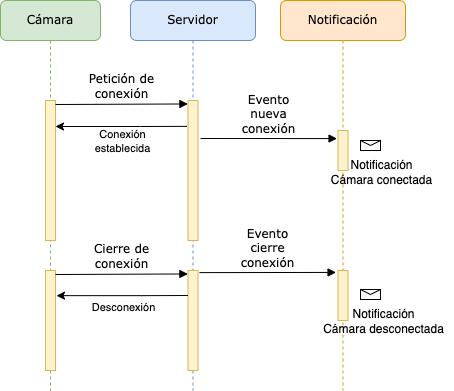
\includegraphics[width=10cm]{img/capitulo_4/camera_notif.png}
    \end{center}
    \begin{center}
        \caption{Diagrama de secuencia: Notificación de conexión/desconexión.}
        Fuente: Elaboración propia.
        \label{fig:diag_sec_notif_conn}
    \end{center}
\end{figure}

A continuación se describe la interacción entre la cámara, el servidor y el proceso de notificación:
\begin{enumerate}
    \item El módulo de cámaras realiza una petición de conexión al servidor.
    \item El servidor responde la petición aceptando la conexión con la designación de un puerto.
    \item El servidor registra el identificador, hora y fecha de conexión de la cámara.
    \item El servidor prepara la notificación con los datos registrados e información sobre otras cámaras disponibles.
    \item El servidor envia notificación por correo electrónico a la dirección configurada.
    \item El servidor prepara el correo electrónico con los datos registrados, información sobre otras cámaras disponibles anteriormente y se envia a la dirección configurada.
    \item El módulo de cámaras se desconecta y se registra fecha y hora de la desconexión.
    \item El servidor prepara la notificación con la fecha y hora de desconexión con información adicional de cámaras disponibles.
    \item El servidor envia la notificación por correo electrónico.
\end{enumerate}

En la figura \ref{fig:diag_sec_dec_fuego} se visualiza el diagrama de secuencia para la detección y notificación de la presencia de fuego.

\begin{figure}[H]
    \begin{center}
        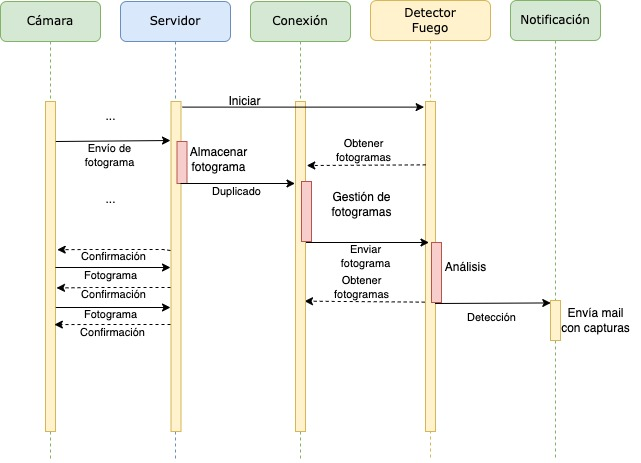
\includegraphics[width=14cm]{img/capitulo_4/fire_detector.jpg}
    \end{center}
    \begin{center}
        \caption{Diagrama de secuencia: Detector de fuego.}
        Fuente: Elaboración propia.
        \label{fig:diag_sec_dec_fuego}
    \end{center}
\end{figure}

A continuación se describe el diagrama de secuencia de la notificación de identificación de fuego.\\
\begin{enumerate}
    \item El servidor inicializa el detector de fuego.
    \item El módulo de cámaras envia un fotograma.    
    \item El servidor recibe el fotograma, almacena en memoria y duplica para el detector de fuego.
    \item El detector requiere un fotograma para su análisis.
    \item El detector de fuego obtiene el fotograma y aplica el análisis.
    \item Si existe una incidencia en el fotograma se almacena como posible evento. 
    \item El detector continua obteniendo fotogramas, analizando cada uno.
    \item Cuando hay un numero determinado de incidencias en los fotogramas se prepara la notificación.
    \item Se envia la notificación por medio de correo electrónico con capturas adjuntas de los fotogramas con incidencias.
\end{enumerate}

En la figura \ref{fig:diag_sec_dec_human} se visualiza el diagrama de secuencia para la detección y notificación de la presencia de intrusos en base a la silueta huamana.

\begin{figure}[H]
    \begin{center}
        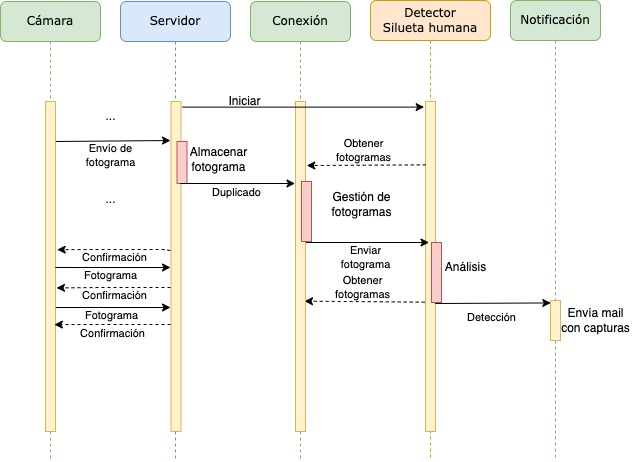
\includegraphics[width=14cm]{img/capitulo_4/human_detection.jpg}
    \end{center}
    \begin{center}
        \caption{Diagrama de secuencia: Detector de silueta humana.}
        Fuente: Elaboración propia.
        \label{fig:diag_sec_dec_human}
    \end{center}
\end{figure}

A continuación se describe el diagrama de secuencia de la notificación de identificación de silueta humana.\\
\begin{enumerate}
    \item El servidor inicializa el detector de silueta humana.
    \item El módulo de cámaras envia un fotograma.    
    \item El servidor recibe el fotograma, almacena en memoria y duplica para el detector.
    \item El detector requiere un fotograma para su análisis.
    \item El detector de silueta humana obtiene el fotograma y aplica el análisis.
    \item Si existe una incidencia en el fotograma se almacena como posible evento. 
    \item El detector continua obteniendo fotogramas, analizando cada uno.
    \item Cuando hay un número determinado de incidencias en los fotogramas se prepara la notificación.
    \item Se envia la notificación por medio de correo electrónico con capturas adjuntas de los fotogramas con incidencias.
\end{enumerate}

En la figura \ref{fig:diag_sec_dec_movimiento} se visualiza el diagrama de secuencia para la detección y notificación de movimiento.

\begin{figure}[H]
    \begin{center}
        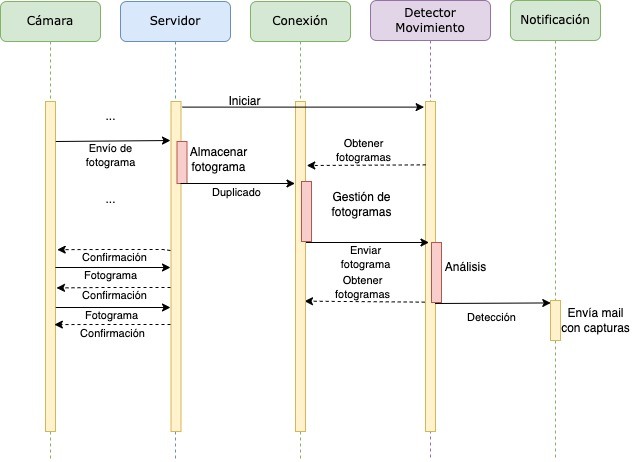
\includegraphics[width=13cm]{img/capitulo_4/movement_detection.jpg}
    \end{center}
    \begin{center}
        \caption{Diagrama de secuencia: Detector de movimiento.}
        Fuente: Elaboración propia.
        \label{fig:diag_sec_dec_movimiento}
    \end{center}
\end{figure}

A continuación se describe el diagrama de secuencia de la notificación de identificación de movimiento.\\
\begin{enumerate}
    \item El servidor inicializa el detector de movimiento.
    \item El módulo de cámaras envia un fotograma.    
    \item El servidor recibe el fotograma, almacena en memoria y duplica para el detector de movimiento.
    \item El detector requiere un fotograma para su análisis.
    \item El detector de fuego obtiene el fotograma y aplica el análisis.
    \item Si existe una incidencia en el fotograma se almacena como posible evento. 
    \item El detector continua obteniendo fotogramas, analizando cada uno.
    \item Cuando hay un numero determinado de incidencias en los fotogramas se prepara la notificación.
    \item Se envia la notificación por medio de correo electrónico con capturas adjuntas de los fotogramas con incidencias.
\end{enumerate}

En la figura \ref{fig:diag_sec_streamming} se visualiza el diagrama de secuencia para la transmisión de video en vivo.

\begin{figure}[H]
    \begin{center}
        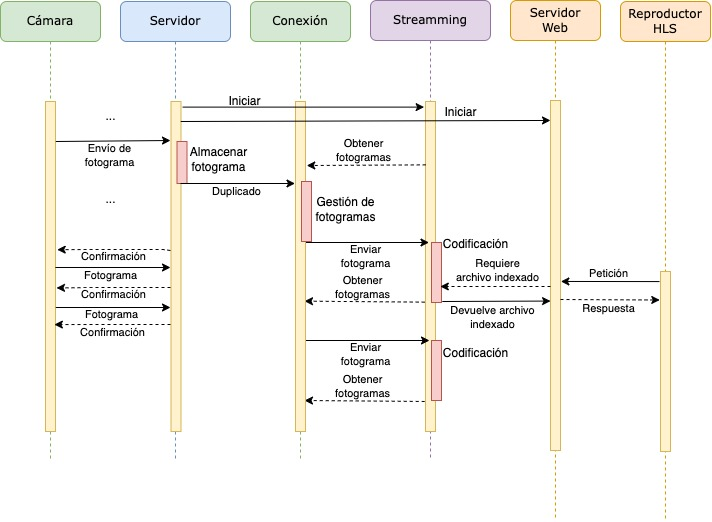
\includegraphics[width=16cm]{img/capitulo_4/stream_secuense.jpg}
    \end{center}
    \begin{center}
        \caption{Diagrama de secuencia: Streamming de video en vivo.}
        Fuente: Elaboración propia.
        \label{fig:diag_sec_streamming}
    \end{center}
\end{figure}

A continuación se describe el diagrama de secuencia de la transmisión en vivo del video generado por el módulo de cámaras.

\begin{enumerate}
    \item El servidor inicia el servicio de Streamming.
    \item El servidor inicia el servidor web para la reproducción desde el navegador.
    \item El módulo de cámaras envia los fotogramas hacia el servidor.
    \item El servidor almacena los fotogramas y gestiona los duplicados.
    \item El servicio de streamming, obtiene los fotogramas para codificar el video y crear la lista de reproducción de los fragmentos de video que son creados.
    \item El servidor web esta a la espera de peticiones cuando se acceda a la dirección específica de la transmision.
    \item La reproducción en vivo comienza cuando se accede a la dirección y el reproductor realiza las peticiones al servidor web.
\end{enumerate}


\subsection{Diagrama de clases}
En la figura \ref{fig:diag_clases_server} se muestra el diagrama de clases del servidor.\\

\begin{figure}[H]
    \begin{center}
        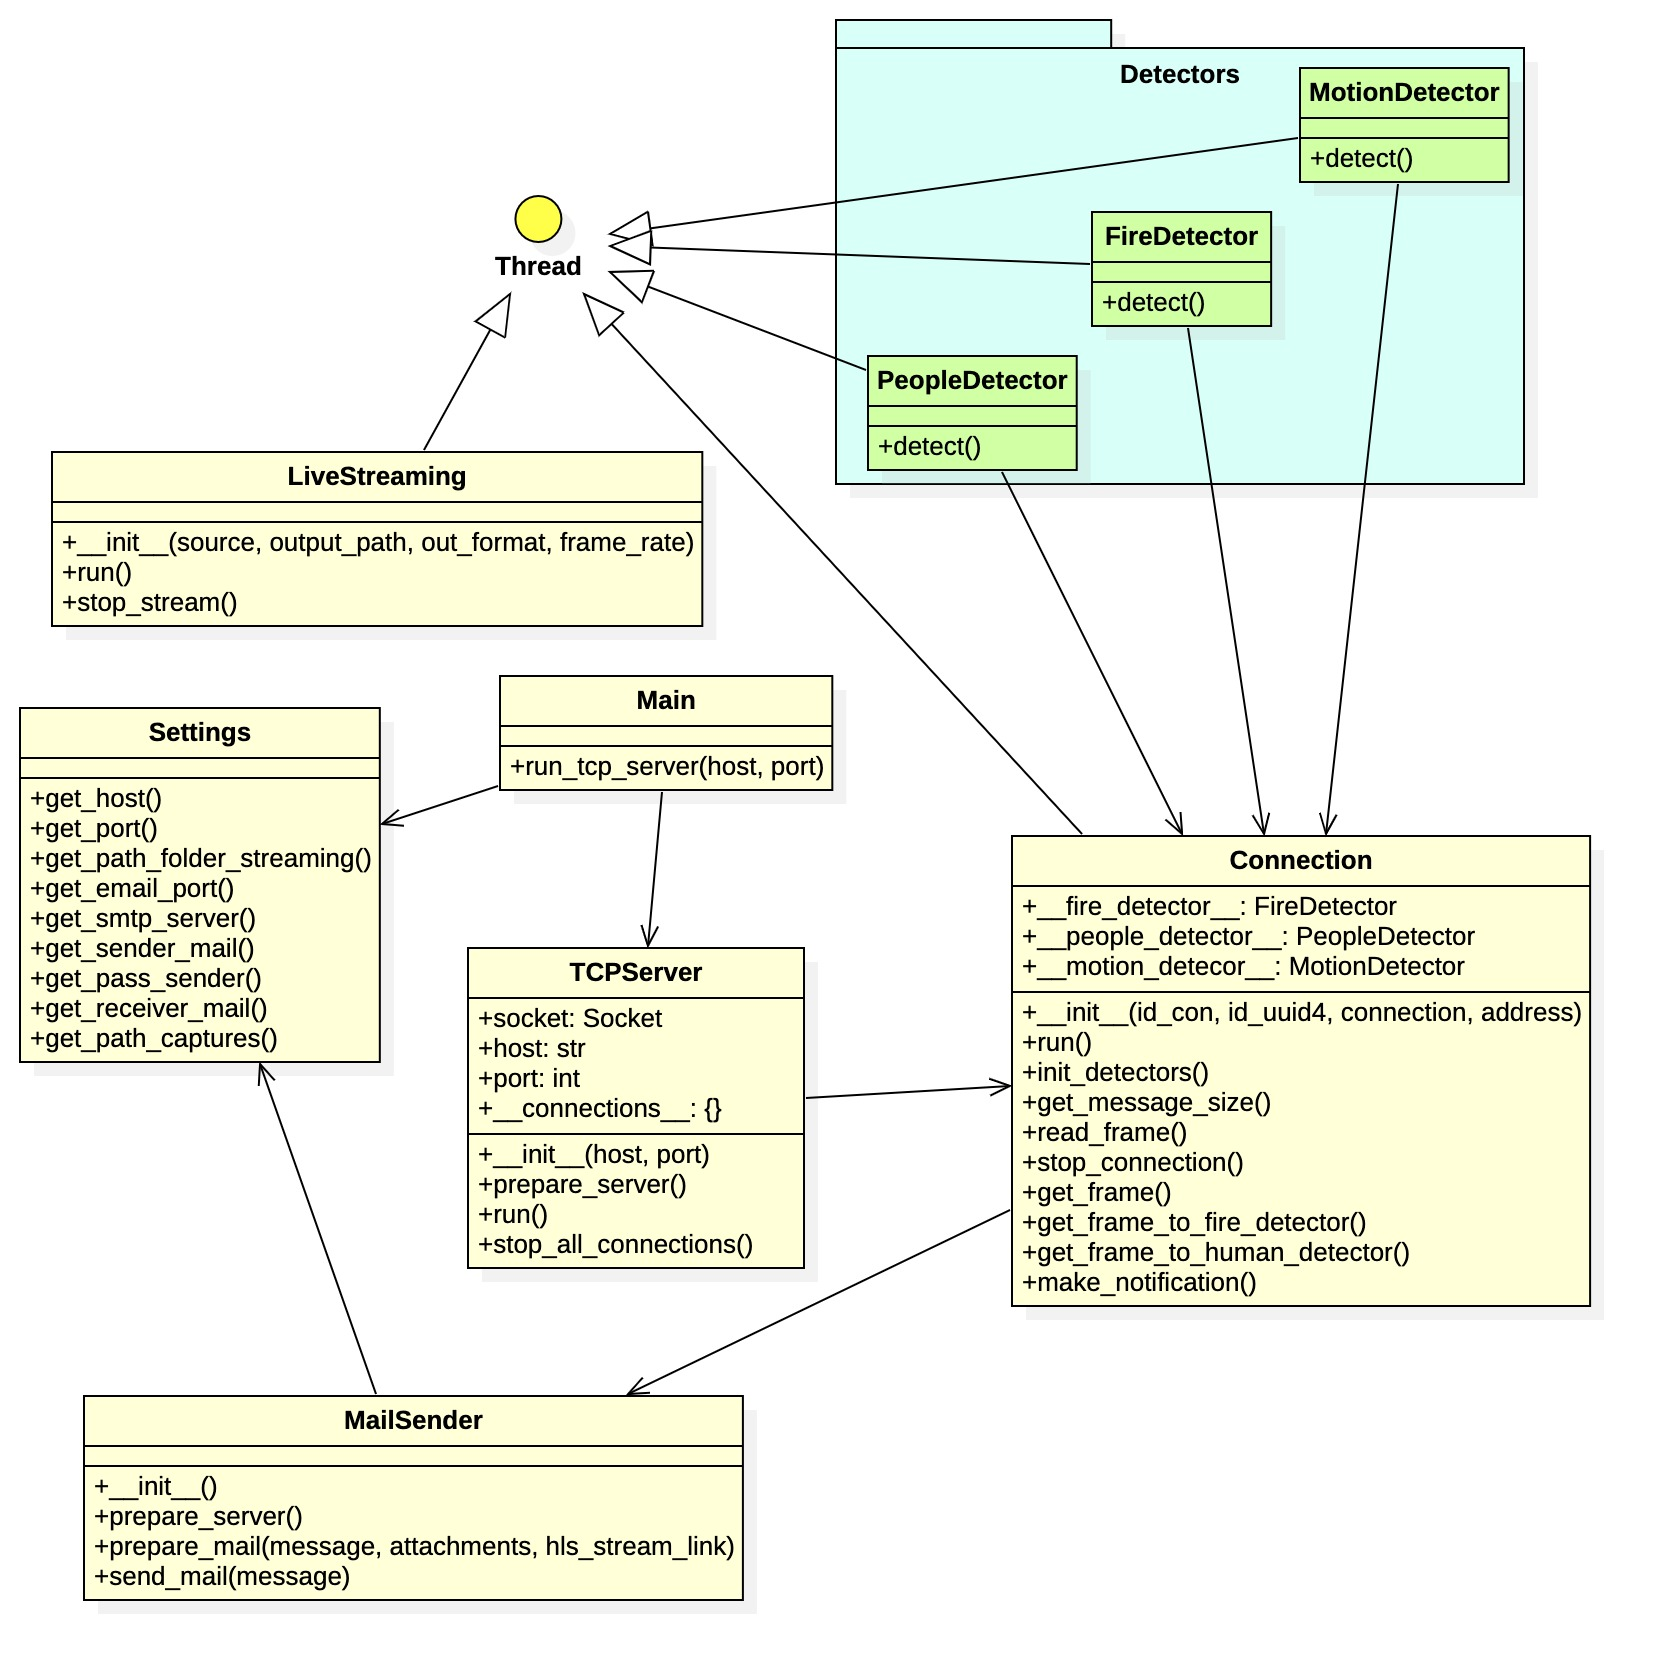
\includegraphics[width=18cm]{img/capitulo_4/tcpserver.jpg}
    \end{center}
    \begin{center}
        \caption{Diagrama de clases: Servidor}
        Fuente: Elaboración propia.
        \label{fig:diag_clases_server}
    \end{center}
\end{figure}

\begin{itemize}
    
    \item \textbf{Main}: Es la clase principal que permite la ejecución constante del servidor. El único método de clase es:
        \begin{itemize}
            \item \textbf{run\_tcp\_server}: Inicializa el servidor en la dirección y puerto provistas desde la configuración.
        \end{itemize}
    \item \textbf{TCPServer}: Clase que maneja las peticiones de nuevas conexiones del módulo de cámaras; prepara el servidor y registra las nuevos procesos que se crean a partir de una nueva conexión. Los atributos de clase son:
        \begin{itemize}
            \item \textbf{socket}: Es la libreria que permite las conexiónes a sistemas externos.
            \item \textbf{host}: Representa la dirección de escucha del servidor.
            \item \textbf{port}: Representa el puerto general de escucha del servidor.
            \item \textbf{connections}: Almacena los nuevos hilos de conexión cuando una nueva cámara se conecta.
        \end{itemize}
        Los métodos de clase son:
        \begin{itemize}
            \item \textbf{prepare\_server}: Método encargado de preparar las configuraciones del servidor antes de empezar su ejecución.
            \item \textbf{run}: Lanza la ejecución del servidor.
            \item \textbf{stop\_all\_connections}: Cierra todas las conexiónes existentes en el momento de cerrar el servidor.
        \end{itemize}
    \item \textbf{Settings}: Clase que se encarga de gestionar todos los valores de configuración en el servidor. Estos son sus métodos de clase:
        \begin{itemize}
            \item \textbf{get\_host}: Obtiene la dirección por defecto desde el archivo de configuración.
            \item \textbf{get\_port}: Obtiene el puerto por defecto desde el archivo de configuración.
            \item \textbf{get\_path\_folder\_streaming}: Obtiene el directorio por defecto para el streamming de video de las cámaras desde el archivo de configuración.
            \item \textbf{get\_email\_port}: Obtiene el puerto del servicio de correo electrónico desde el archivo de configuración.
            \item \textbf{get\_smtp\_server}: Obtiene la dirección por defecto del servicio de correo electrónico desde el archivo de configuración.
            \item \textbf{get\_sender\_mail}: Obtiene a dirección de correo electrónico para el envío de correos de notificación. 
            \item \textbf{get\_pass\_sender}: Obtiene la contraseña del correo electrónico para el envío de correos de notificación. 
            \item \textbf{get\_receiver\_mail}: Obtiene la dirección de correo electronico destino.
            \item \textbf{get\_path\_captures}: Obtiene el directorio por defecto de las capturas de los detectores desde el archivo de configuración.
        \end{itemize}
    \item \textbf{Connection}: Clase encargada de gestionar, duplicar y almacenar los fotogramas que son enviados desde el módulo de cámaras. Sus propiedades son:
        \begin{itemize}
            \item \textbf{fire\_detector}: Instancia de la clase del detector de fuego.
            \item \textbf{people\_detector}: Instancia de la clase del detector de silueta humana.
            \item \textbf{motion\_detector}: Instancia de la clase del detector de movimiento.
        \end{itemize}
        Sus métodos de clase son:
        \begin{itemize}
            \item \textbf{run}: Ejecuta el proceso de escucha y gestion de nuevas conexiones por parte del módulo de cámaras.
            \item \textbf{init\_detectors}: Lanza los procesos de detección.
            \item \textbf{get\_message\_size}: Obtiene el valor del tamaño de los mensajes para procesar las capturas recibidas por el módulo de cámaras.
            \item \textbf{read\_frame}: Recibe el fotograma y convierte la información de un valor binario a imagen
            \item \textbf{stop\_connection}: Cierre el proceso de conexión del módulo de cámaras y procesos de detección.
            \item \textbf{get\_frame}: Devuelve un fotograma hacia los detectores o al módulo de transmisión de video en vivo.
            \item \textbf{store\_frame}: Almacena en memoria un fotograma.
            \item \textbf{make\_notification}: Prepara y envia la notificación a partir de la señal de un detector.
        \end{itemize}
    \item \textbf{LiveStreamming}: Clase que se encarga de la codificación y decodificación de video, construyendo el archivo que registra los fragmentos de video creados para su transmisión:
        \begin{itemize}
            \item \textbf{init}: Inicializa el módulo de transmisión de video en vivo.
            \item \textbf{run}: Ejecuta de manera constante el decodificado del video.
            \item \textbf{stop\_stream}: Termina la transmisión y cierra el proceso de codificación.
        \end{itemize}
    \item \textbf{MailSender}: Clase encargada de ofrecer el servicio de envio de mensajes por correo electrónico:
        \begin{itemize}
            \item \textbf{init}: Inicia el módulo de envio de correo electrónico.
            \item \textbf{prepare\_server}: Prepara el servicio de correo electrónico a partir de los valores de configuración.
            \item \textbf{prepare\_mail}: Prepara el mensaje de correo a partir del detector que genera la alarma.
            \item \textbf{send\_mail}: Envia el correo electrónico a la dirección registrada en el archivo de configuraciones.
        \end{itemize}
    \item \textbf{PeopleDetector}: Clase encargada de la detección de siluetas humana en los fotogramas. Este es el único método de clase:
        \begin{itemize}
            \item \textbf{detect}: Método que se encarga de aplicar el algoritmo de detección de siluetas humanas sobre los fotogramas.
        \end{itemize}
    \item \textbf{FireDetector}: Clase encargada de la detección de fuego en los fotogramas. Este es el único método de clase:
        \begin{itemize}
            \item \textbf{detect}: Método que se encarga de aplicar el algoritmo de detección de fuego sobre los fotogramas.
        \end{itemize}
    \item \textbf{MotionDetector}: Clase encargada de la detección de movimiento en los fotogramas. Este es el único método de clase:
        \begin{itemize}
            \item \textbf{detect}: Método que se encarga de aplicar el algoritmo de detección de movimiento sobre los fotogramas.
        \end{itemize}
\end{itemize}

\section{Diseño de notificación por correo electrónico}
Cuando se identifica un evento por parte de alguno de los tres detectores implementados, es necesario notificar al usuario; el medio elegido es un correo electrónico que debe ser más que solo un texto referente a la identificación de un suceso. Se diseña un mensaje con texto enriquecido adjuntando mayor información en el momento de:
\begin{itemize}
    \item Conectar una cámara del módulo de cámaras al servidor.
    \item Desconectar una cámara del módulo de cámaras al servidor.
    \item Identificación de fuego en fotogramas.
    \item Identificación de silueta humana en los fotogramas.
    \item Identificación de movimiento en los fotogramas.
\end{itemize}
Además de agregar información sobre la fecha y hora de conexión/desconexión o identificación de algun suceso; se adjunta capturas acorde a lo identificado. A continuación se detalla cada uno de los ejemplos de notificación a desarrollar.

\begin{itemize}
    \item En la figura \ref{fig:desing_cam_conn_more_cams}, se detalla la conexión de una cámara y se muestra información de otras cámaras disponibles.

    \begin{figure}[H]
        \begin{center}
            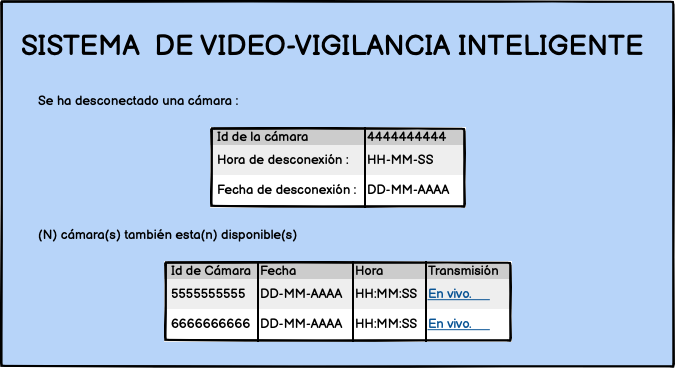
\includegraphics[width=10cm]{img/capitulo_4/cam_connected_more_cams.png}
        \end{center}
        \begin{center}
            \caption{Diseño de notificación: Conecta una cámara más al sistema.}
            Fuente: Elaboración propia.
            \label{fig:desing_cam_conn_more_cams}
        \end{center}
    \end{figure}
    
    \item En la figura \ref{fig:desing_cam_conn_no_more_cams}, se detalla la desconexión de una cámara y no existen cámaras disponibles.
    
    \begin{figure}[H]
        \begin{center}
            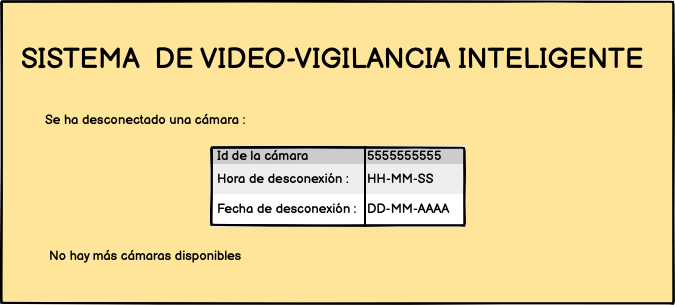
\includegraphics[width=10cm]{img/capitulo_4/cam_connected_no_more_cams.png}
        \end{center}
        \begin{center}
            \caption{Diseño de notificación: Desconexión de la única cámara.}
            Fuente: Elaboración propia.
            \label{fig:desing_cam_conn_no_more_cams}
        \end{center}
    \end{figure}
    
    \item En la figura \ref{fig:desing_cam_disconn_more_cams}, se detalla la desconexión de una cámara y existen otras cámaras disponibles.
    \begin{figure}[H]
        \begin{center}
            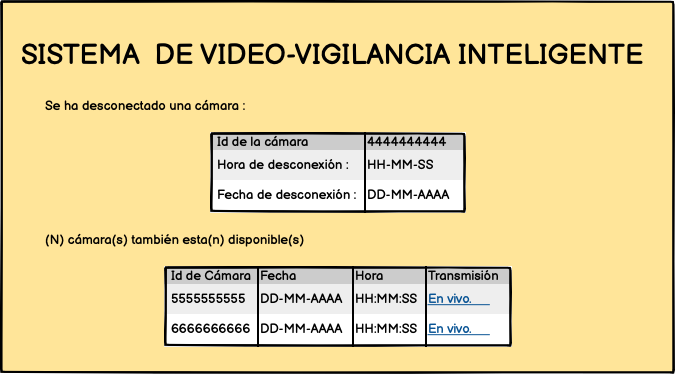
\includegraphics[width=10cm]{img/capitulo_4/cam_disconnected_more_cams.png}
        \end{center}
        \begin{center}
            \caption{Diseño de notificación: Desconexión de una de las cámaras disponibles.}
            Fuente: Elaboración propia.
            \label{fig:desing_cam_disconn_more_cams}
        \end{center}
    \end{figure}
    
    \item En la figura \ref{fig:desing_cam_disconn_no_more_cams}, se detalla la conexión de una cámara y no existen otras cámaras disponibles.
    \begin{figure}[H]
        \begin{center}
            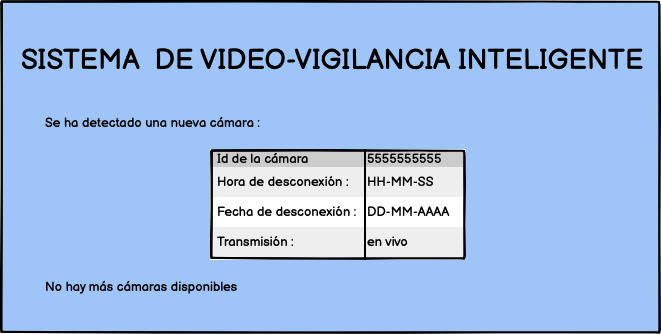
\includegraphics[width=9cm]{img/capitulo_4/cam_disconnected_no_more_cams.png}
        \end{center}
        \begin{center}
            \caption{Diseño de notificación: Nueva y única conexión.}
            Fuente: Elaboración propia.
            \label{fig:desing_cam_disconn_no_more_cams}
        \end{center}
    \end{figure}    

    \item En la figura \ref{fig:desing_fire_detection_notif}, se muestra el ejemplo de notificación de identificación de fuego.
    \begin{figure}[H]
        \begin{center}
            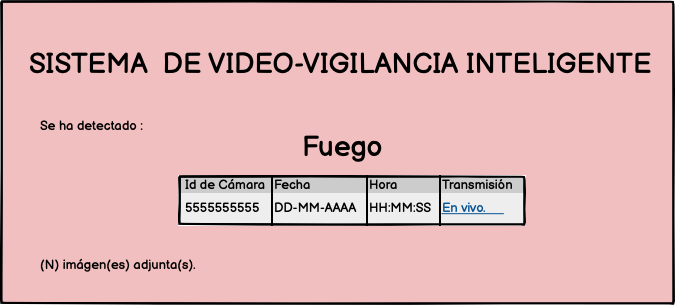
\includegraphics[width=10cm]{img/capitulo_4/fire_detection_mail.png}
        \end{center}
        \begin{center}
            \caption{Diseño de notificación: Fuego detectado.}
            Fuente: Elaboración propia.
            \label{fig:desing_fire_detection_notif}        
        \end{center}
    \end{figure}
    
    \item En la figura \ref{fig:desing_human_detection_notif}, se muestra el ejemplo de notificación de identificación de silueta humana.
    
    \begin{figure}[H]
        \begin{center}
            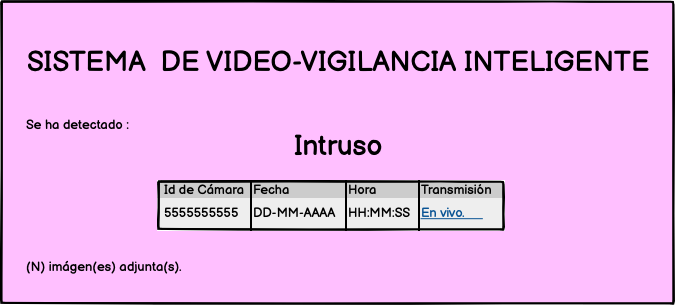
\includegraphics[width=10cm]{img/capitulo_4/human_detection_mail.png}
        \end{center}
        \begin{center}
            \caption{Diseño de notificación: Silueta humana detectada.}
            Fuente: Elaboración propia.
            \label{fig:desing_human_detection_notif}
        \end{center}
    \end{figure}    

    \item En la figura \ref{fig:desing_motion_detection_notif}, se muestra el ejemplo de notificación de identificación de movimiento.
    \begin{figure}[H]
        \begin{center}
            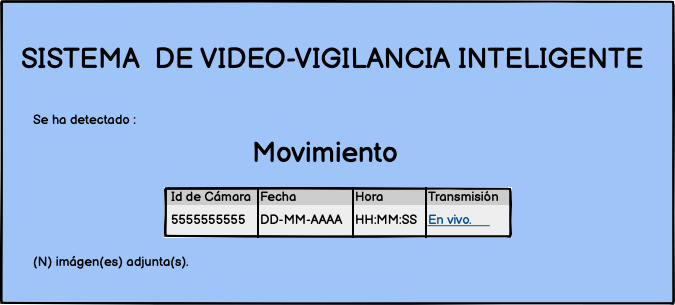
\includegraphics[width=10cm]{img/capitulo_4/movement_detection_mail.png}
        \end{center}
        \begin{center}
            \caption{Diseño de notificación: Movimiento detectado.}
            Fuente: Elaboración propia.
            \label{fig:desing_motion_detection_notif}
        \end{center}
    \end{figure}
\end{itemize}

    \chapter{Implementación}
En este capitulo se describe a detalle el proceso de implementación de los diferentes módulos que forman parte del sistema  de video-vigilancia inteligente.

\section{Módulo de Cámara}
\subsection{Diseño de clases}
\subsection{Diseño de interfaz de simulador}
\subsection{Captura de video}
\subsection{Conexión a Servidor TCP}
\subsection{Comunicacion y envío de fotogramas}
\section{Módulo de Servidor TCP}
\subsection{Diseño de clases}
\subsection{Manejador de conectores de clientes}
\subsection{Streamming HLS}
\subsection{Detectores}
\subsubsection{Detector de movimiento}
\subsubsection{Detector de intrusos}
\subsubsection{Detector de fuego/humo}
\section{Servidor HTTP}
\section{Modulo de envío de correo electrónico}

\begin{longtable}{p{2cm}|p{3cm}|p{3cm}|p{3cm}|p{3cm}|}
    \caption{Titulo de tabla multipágina} \label{tabla:tabla_largo_ejemplo} \\
    \cline{2-5}
    \multicolumn{1}{l|}{} & \multicolumn{1}{c|}{\textbf{Columna 1}} & \multicolumn{1}{c|}{\textbf{Columna 2}} & \multicolumn{1}{c|}{\textbf{Columna 3}} & \multicolumn{1}{c|}{\textbf{Columna 4}}\\ \hline
    \endfirsthead

    \multicolumn{5}{c}{{\tablename{} \thetable{} -- Continuación de tabla previa}} \\
    \multicolumn{5}{l}{} \\
    \cline{2-5}
    \multicolumn{1}{l|}{} & \multicolumn{1}{c|}{\textbf{Columna 1}} & \multicolumn{1}{c|}{\textbf{Columna 2}} & \multicolumn{1}{c|}{\textbf{Columna 3}} & \multicolumn{1}{c|}{\textbf{Columna 4}}\\ \hline
    \endhead

    \multicolumn{5}{c}{{Continua en la siguiente página.}} \\
    \endfoot

    \multicolumn{5}{l}{} \\
    \multicolumn{5}{l}{Nota. Extraída de Apellido, N. (2000) \textit{Nombre del libro}. Editorial o universidad que lo publicó.} \\
    \endlastfoot

    \multicolumn{1}{|c|}{\textbf{Fila 1}} & Lorem ipsum dolor sit amet, consectetuer adipiscing elit. & Lorem ipsum dolor sit amet, consectetuer adipiscing elit. & Lorem ipsum dolor sit amet, consectetuer adipiscing elit. & Lorem ipsum dolor sit amet, consectetuer adipiscing elit. \\ \hline
    \multicolumn{1}{|c|}{\textbf{Fila 2}} & Lorem ipsum dolor sit amet, consectetuer adipiscing elit. & Lorem ipsum dolor sit amet, consectetuer adipiscing elit. & Lorem ipsum dolor sit amet, consectetuer adipiscing elit. & Lorem ipsum dolor sit amet, consectetuer adipiscing elit. \\ \hline
    \multicolumn{1}{|c|}{\textbf{Fila 3}} & Lorem ipsum dolor sit amet, consectetuer adipiscing elit. & Lorem ipsum dolor sit amet, consectetuer adipiscing elit. & Lorem ipsum dolor sit amet, consectetuer adipiscing elit. & Lorem ipsum dolor sit amet, consectetuer adipiscing elit. \\ \hline
    \multicolumn{1}{|c|}{\textbf{Fila 4}} & Lorem ipsum dolor sit amet, consectetuer adipiscing elit. & Lorem ipsum dolor sit amet, consectetuer adipiscing elit. & Lorem ipsum dolor sit amet, consectetuer adipiscing elit. & Lorem ipsum dolor sit amet, consectetuer adipiscing elit. \\ \hline
    \multicolumn{1}{|c|}{\textbf{Fila 5}} & Lorem ipsum dolor sit amet, consectetuer adipiscing elit. & Lorem ipsum dolor sit amet, consectetuer adipiscing elit. & Lorem ipsum dolor sit amet, consectetuer adipiscing elit. & Lorem ipsum dolor sit amet, consectetuer adipiscing elit. \\ \hline
    \multicolumn{1}{|c|}{\textbf{Fila 6}} & Lorem ipsum dolor sit amet, consectetuer adipiscing elit. & Lorem ipsum dolor sit amet, consectetuer adipiscing elit. & Lorem ipsum dolor sit amet, consectetuer adipiscing elit. & Lorem ipsum dolor sit amet, consectetuer adipiscing elit. \\ \hline  
    \multicolumn{1}{|c|}{\textbf{Fila 7}} & Lorem ipsum dolor sit amet, consectetuer adipiscing elit. & Lorem ipsum dolor sit amet, consectetuer adipiscing elit. & Lorem ipsum dolor sit amet, consectetuer adipiscing elit. & Lorem ipsum dolor sit amet, consectetuer adipiscing elit. \\ \hline    
    \multicolumn{1}{|c|}{\textbf{Fila 8}} & Lorem ipsum dolor sit amet, consectetuer adipiscing elit. & Lorem ipsum dolor sit amet, consectetuer adipiscing elit. & Lorem ipsum dolor sit amet, consectetuer adipiscing elit. & Lorem ipsum dolor sit amet, consectetuer adipiscing elit. \\ \hline    
    \multicolumn{1}{|c|}{\textbf{Fila 9}} & Lorem ipsum dolor sit amet, consectetuer adipiscing elit. & Lorem ipsum dolor sit amet, consectetuer adipiscing elit. & Lorem ipsum dolor sit amet, consectetuer adipiscing elit. & Lorem ipsum dolor sit amet, consectetuer adipiscing elit. \\ \hline    
    \multicolumn{1}{|c|}{\textbf{Fila 10}} & Lorem ipsum dolor sit amet, consectetuer adipiscing elit. & Lorem ipsum dolor sit amet, consectetuer adipiscing elit. & Lorem ipsum dolor sit amet, consectetuer adipiscing elit. & Lorem ipsum dolor sit amet, consectetuer adipiscing elit. \\ \hline    
    \multicolumn{1}{|c|}{\textbf{Fila 11}} & Lorem ipsum dolor sit amet, consectetuer adipiscing elit. & Lorem ipsum dolor sit amet, consectetuer adipiscing elit. & Lorem ipsum dolor sit amet, consectetuer adipiscing elit. & Lorem ipsum dolor sit amet, consectetuer adipiscing elit. \\ \hline    
    \multicolumn{1}{|c|}{\textbf{Fila 12}} & Lorem ipsum dolor sit amet, consectetuer adipiscing elit. & Lorem ipsum dolor sit amet, consectetuer adipiscing elit. & Lorem ipsum dolor sit amet, consectetuer adipiscing elit. & Lorem ipsum dolor sit amet, consectetuer adipiscing elit. \\ \hline    
\end{longtable}

% \section{Módulo Cliente - Aplicación Móvil}
% \subsection{Android}
% \subsection{ExoPlayer}
% \subsection{Notificacion FireBase}
% \subsection{Disenio de Interfaz}
% \subsection{Historial de notificaciones}
    \chapter{Pruebas}

Según la metodologia ``cascada'', la fase final del desarrollo se cierra cuando se realizan pruebas sobre lo implementado en la fase anterior. Para probar en su totalidad el sistema de video-vigilancia se plantean las siguientes pruebas de aceptación.\\

\section{Prueba de conexión del módulo de cámaras}
En la siguiente tabla se describe la prueba realizada:\\

\begin{table}[H]
    \caption{Detalle de prueba de conexión de módulo de cámaras}
    \begin{center}
        \begin{tabular}{|>{\centering}p{0.3\textwidth}|m{0.6\textwidth}<{\centering}|} 
            \hline
            \textbf{Título de la prueba} & Única cámara conectada \\
            \hline
            \textbf{Descripción} & El servidor se encuentra en ejecución y una instancia del módulo de cámaras se conecta al servidor. No existen más cámaras conectadas.\\
            \hline
            \textbf{Comportamiento obtenido} & 
            \begin{itemize}
                \item El servidor registra la desconexión y lo muestra en consola.
                \item El servidor notifica al usuario por medio de correo electronico.
                \item La notificación provee información sobre la fecha y hora de la desconexión.
                \item La notificación detalla que no hay más conexiones.
            \end{itemize} \\ 
            \hline
            \textbf{Estado de prueba} & Exitoso \\
            \hline
        \end{tabular}
    \end{center}
\end{table}

A continuación se muestra las capturas del comportamiento esperado:\\

\begin{figure}[H]
    \begin{center}
        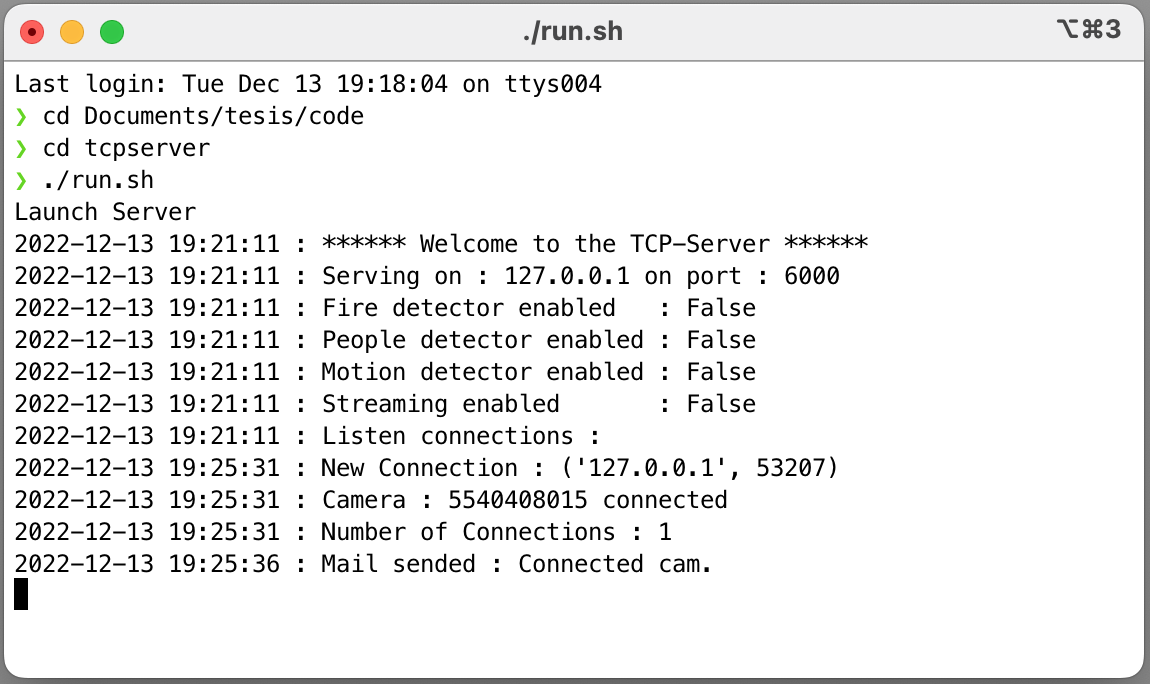
\includegraphics[width=13cm]{img/capitulo_6/server_cam_connected.png}
        \caption{Mensajes en consola del servidor en parte del}
        Fuente : Elaboración propia
    \end{center}
\end{figure}

\begin{figure}[H]
    \begin{center}
        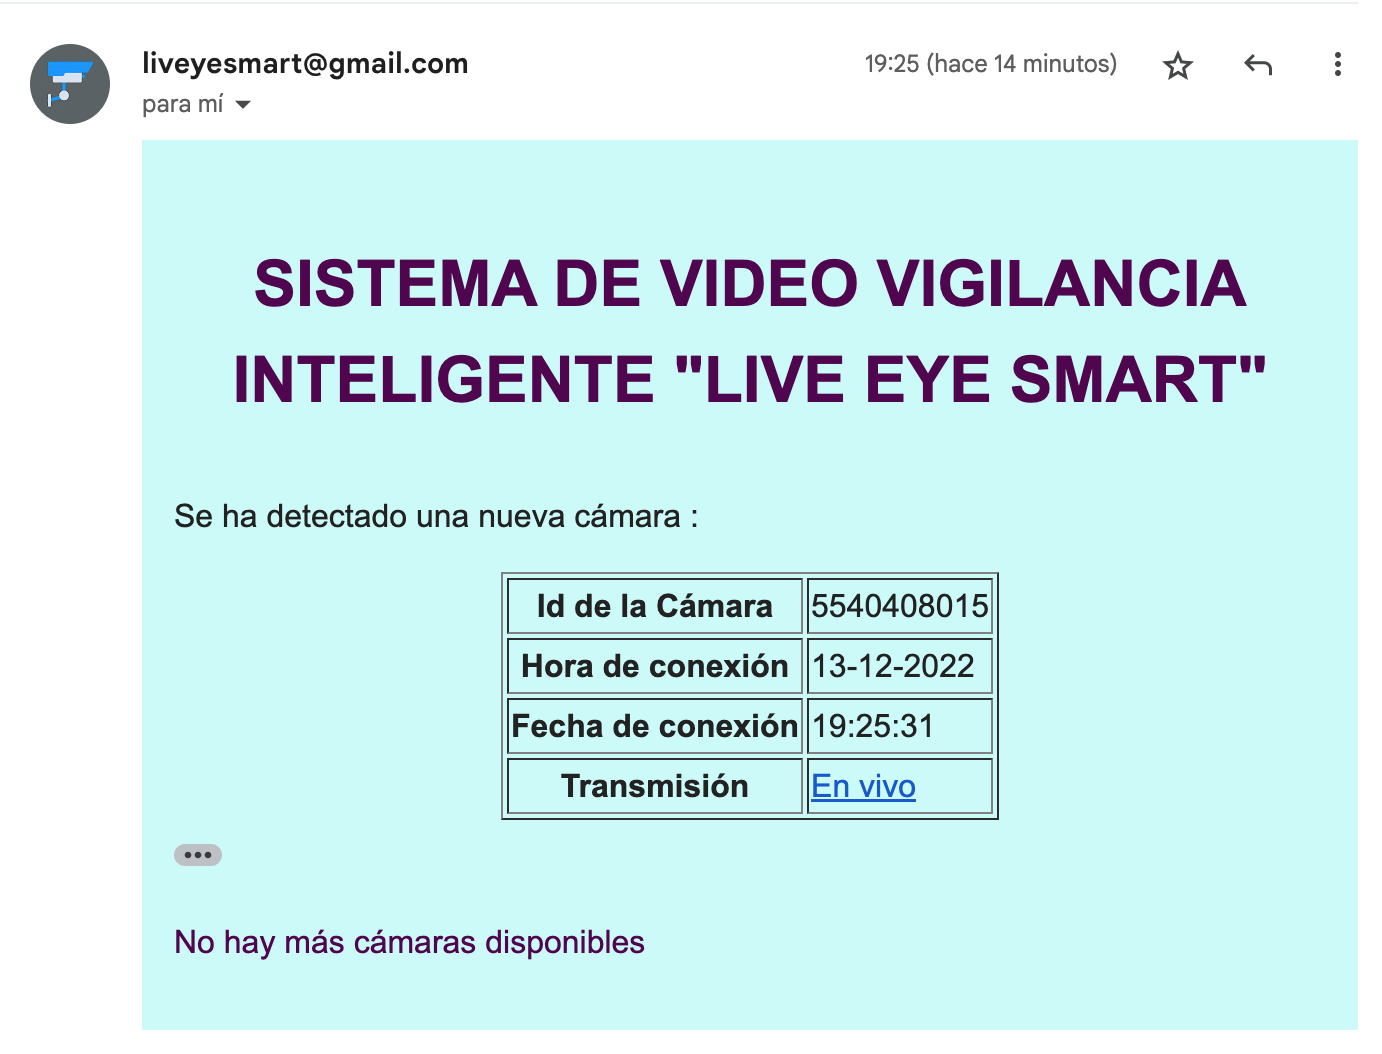
\includegraphics[width=13cm]{img/capitulo_6/mail1.png}
        \caption{Detalle de notificación por correo electrónico.}
        Fuente : Elaboración propia
    \end{center}
\end{figure}

En la siguiente tabla se describe otra de las prueba realizadas:\\

\begin{table}[H]
    \caption{Detalle de prueba de conexión del módulo de cámaras con más de una cámara disponible}
    \begin{center}
        \begin{tabular}{|>{\centering}p{0.3\textwidth}|m{0.6\textwidth}<{\centering}|} 
            \hline
            \textbf{Título de la prueba} & Más de una cámara conectada \\
            \hline
            \textbf{Descripción} & El servidor se encuentra en ejecución y una instancia del módulo de cámaras se conecta al servidor. Existen más de una cámara conectada.\\
            \hline
            \textbf{Comportamiento obtenido} & 
            \begin{itemize}
                \item El servidor acepta la conexión y lo muestra en consola.
                \item El servidor notifica al usuario por medio de correo electronico.
                \item La notificación provee información sobre la fecha y hora de la conexión, compartiendo el enlace para la transmisión en vivo.
                \item La notificación provee la misma información de las demás cámaras conectadas al servidor.
            \end{itemize} \\ 
            \hline
            \textbf{Estado de prueba} & Exitoso \\
            \hline
        \end{tabular}
    \end{center}
\end{table}

A continuación se muestra las capturas del comportamiento esperado:

\begin{figure}[H]
    \begin{center}
        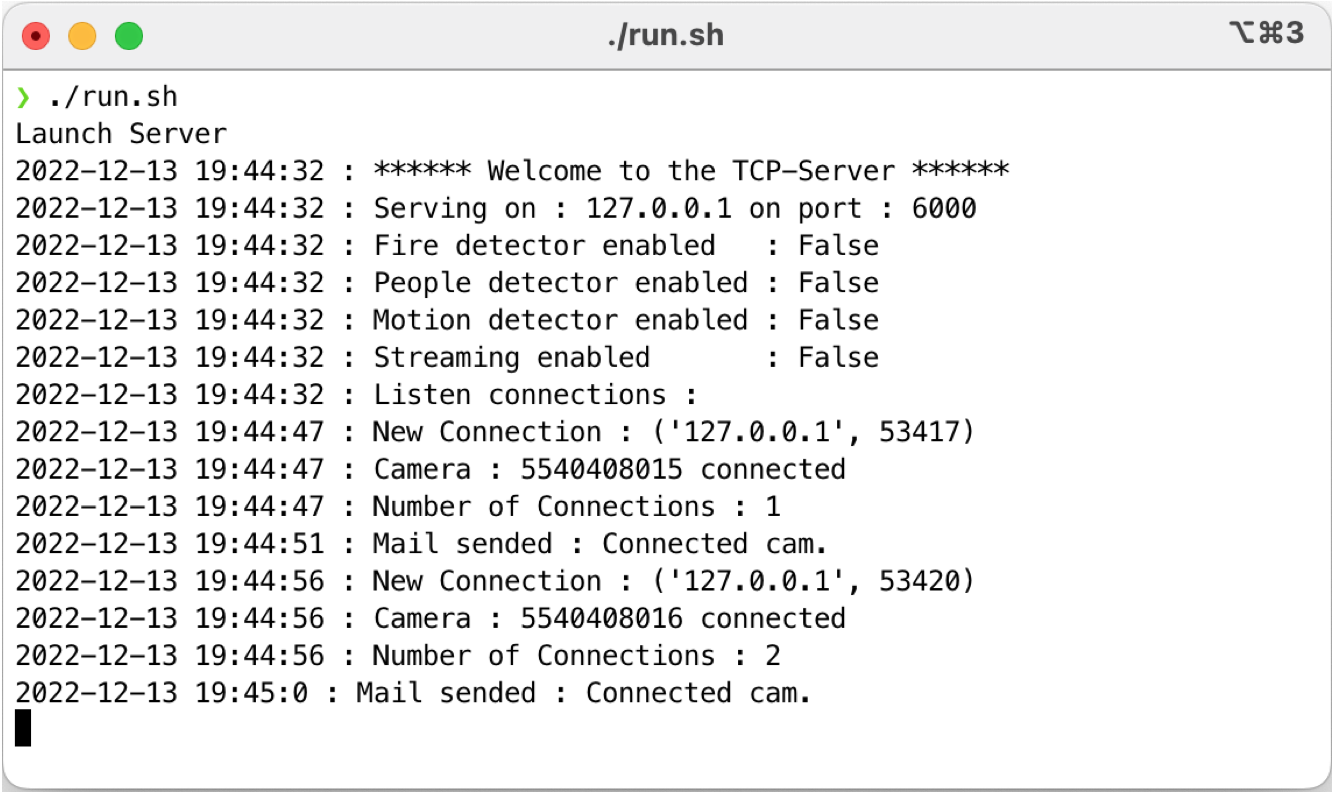
\includegraphics[width=15cm]{img/capitulo_6/server_cam_connected_more_cams.png}
        \caption{Mensajes en consola del servidor}
        Fuente : Elaboración propia
    \end{center}
\end{figure}

\begin{figure}[H]
    \begin{center}
        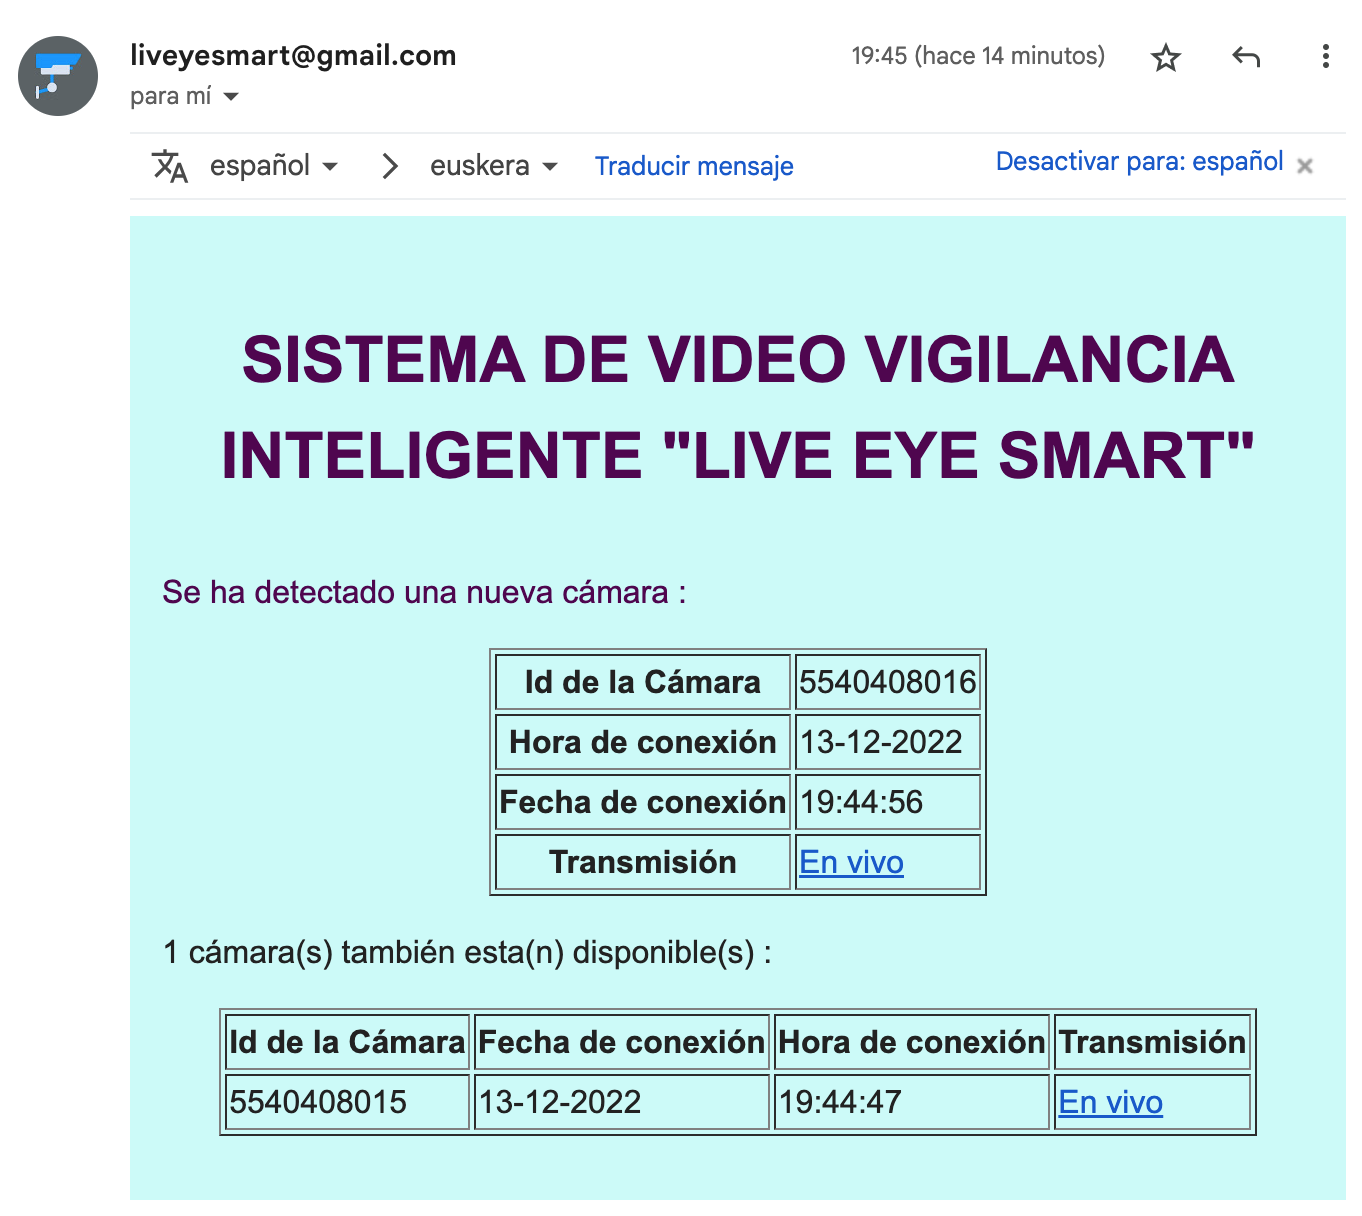
\includegraphics[width=10cm]{img/capitulo_6/mail2.png}
        \caption{Detalle de notificación por correo electrónico.}
        Fuente : Elaboración propia
    \end{center}
\end{figure}


\section{Prueba de desconexión del módulo de cámaras}

En la siguiente tabla se describe una de las pruebas realizadas:\\

\begin{table}[H]
    \caption{Detalle de prueba de desconexión del módulo de cámaras, única cámara conectada}
    \begin{center}
        \begin{tabular}{|>{\centering}p{0.3\textwidth}|m{0.6\textwidth}<{\centering}|} 
            \hline
            \textbf{Título de la prueba} & Única cámara conectada y se desconecta \\
            \hline
            \textbf{Descripción} & El servidor se encuentra en ejecución y la única instancia del módulo de cámaras se desconecta del servidor. No existen más cámaras conectadas.\\
            \hline
            \textbf{Comportamiento obtenido} & 
            \begin{itemize}
                \item El servidor registra la desconexión y lo muestra en consola.
                \item El servidor notifica al usuario por medio de correo electronico.
                \item La notificación provee información sobre la fecha y hora de la desconexión.
                \item La notificación detalla que no hay más conexiones.
            \end{itemize} \\ 
            \hline
            \textbf{Estado de prueba} & Exitoso \\
            \hline
        \end{tabular}
    \end{center}
\end{table}
A continuación se muestra las capturas del comportamiento esperado:\\
\begin{figure}[H]
    \begin{center}
        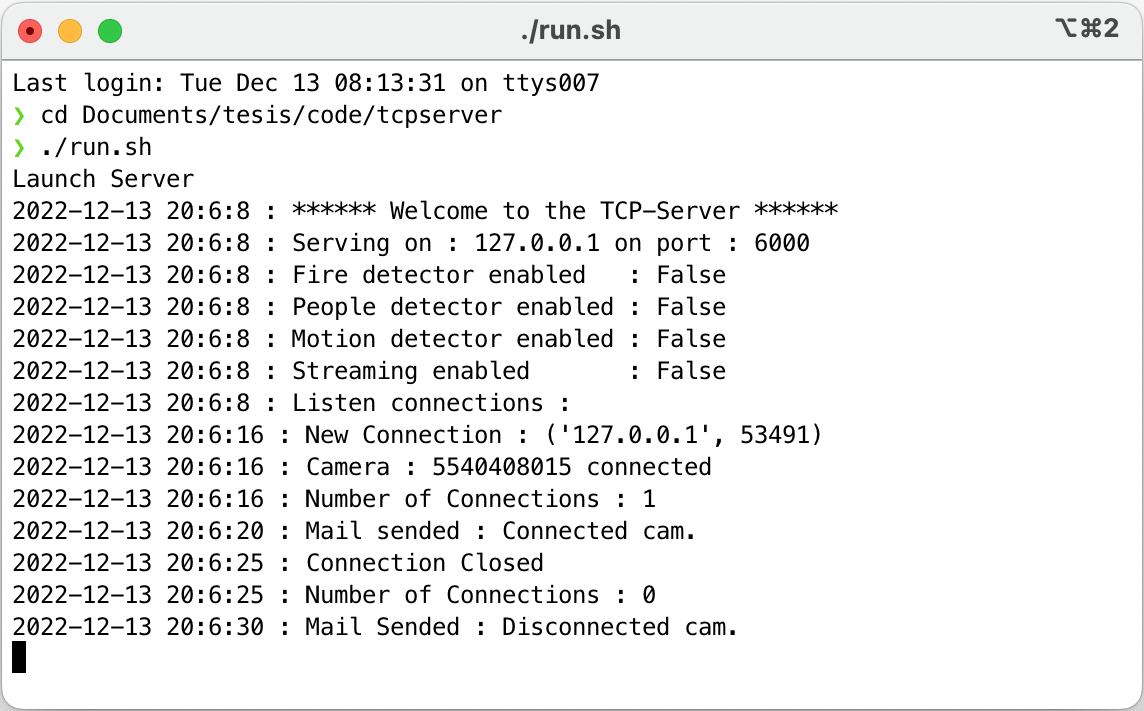
\includegraphics[width=12cm]{img/capitulo_6/cam_disconnected_1_cam.png}
    \end{center}
    \begin{center}
        \caption{Mensajes en consola del servidor}
        Fuente : Elaboración propia
    \end{center}
\end{figure}

\begin{figure}[H]
    \begin{center}
        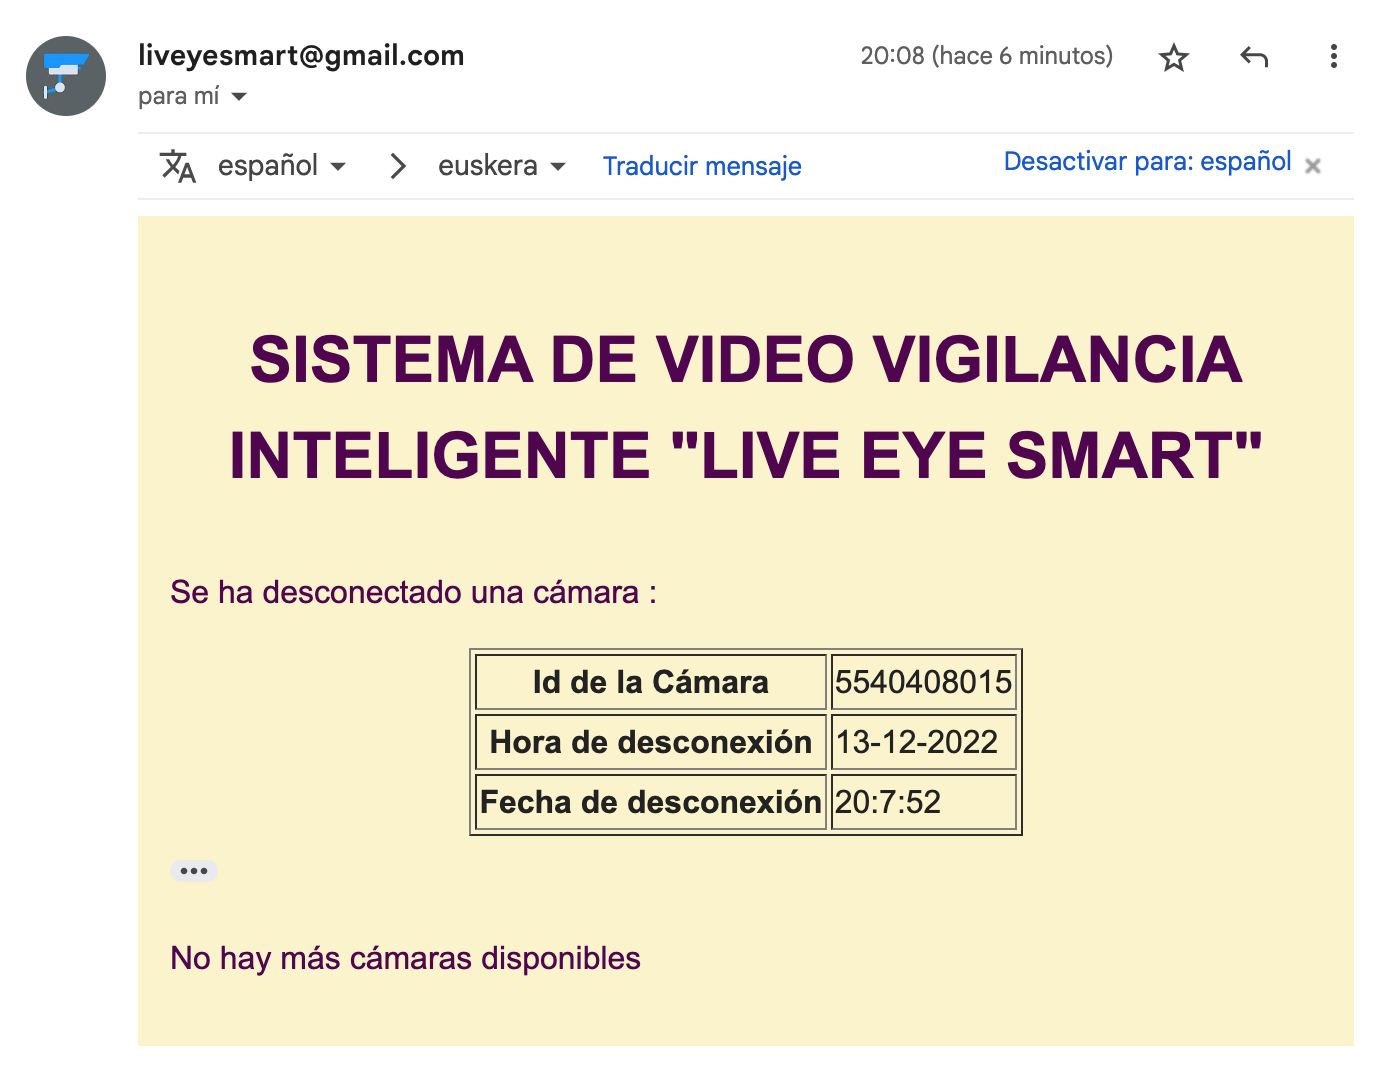
\includegraphics[width=12cm]{img/capitulo_6/mail4.png}
    \end{center}
    \begin{center}
        \caption{Detalle de notificación por correo electrónico.}
        Fuente : Elaboración propia
    \end{center}
\end{figure}

En la siguiente tabla se describe otra de las pruebas realizadas:\\

\begin{table}[H]
    \caption{Detalle de prueba de desconexión de módulo de cámaras con más de una cámara conectada}
    \begin{center}
        \begin{tabular}{|>{\centering}p{0.3\textwidth}|m{0.6\textwidth}<{\centering}|} 
            \hline
            \textbf{Título de la prueba} & Una de las cámaras es desconectada \\
            \hline
            \textbf{Descripción} & El servidor se encuentra en ejecución y una instancia del módulo de cámaras se desconecta del servidor. Existen más cámaras conectadas.\\
            \hline
            \textbf{Comportamiento obtenido} & 
            \begin{itemize}
                \item El servidor acepta la conexión y lo muestra en consola.
                \item El servidor notifica al usuario por medio de correo electronico.
                \item La notificación provee información sobre la fecha y hora de la conexión, compartiendo el enlace para la transmisión en vivo.
            \end{itemize} \\ 
            \hline
            \textbf{Estado de prueba} & Exitoso \\
            \hline
        \end{tabular}
    \end{center}
\end{table}

A continuación se muestra las capturas del comportamiento esperado:

\begin{figure}[H]
    \begin{center}
        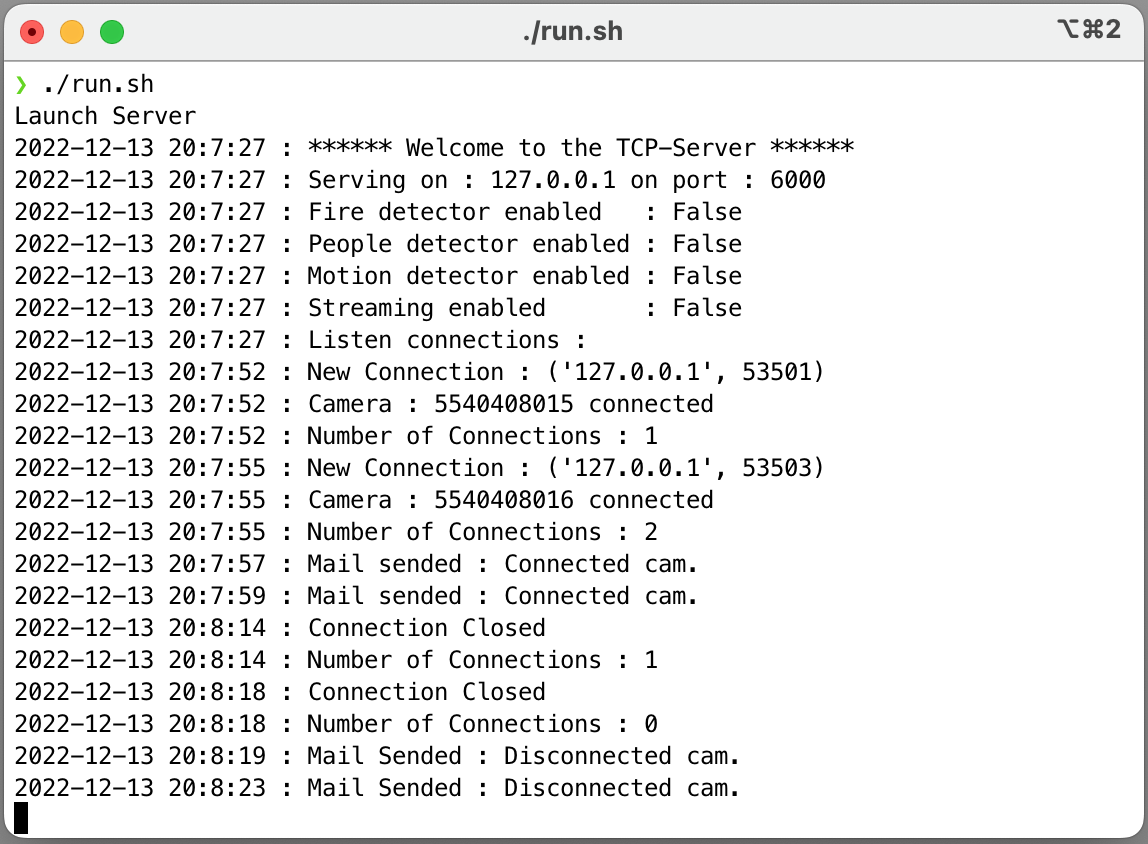
\includegraphics[width=13cm]{img/capitulo_6/cam_disconnected_n_cams.png}
        \caption{Mensajes en consola del servidor}
        Fuente : Elaboración propia
    \end{center}
\end{figure}

\begin{figure}[H]
    \begin{center}
        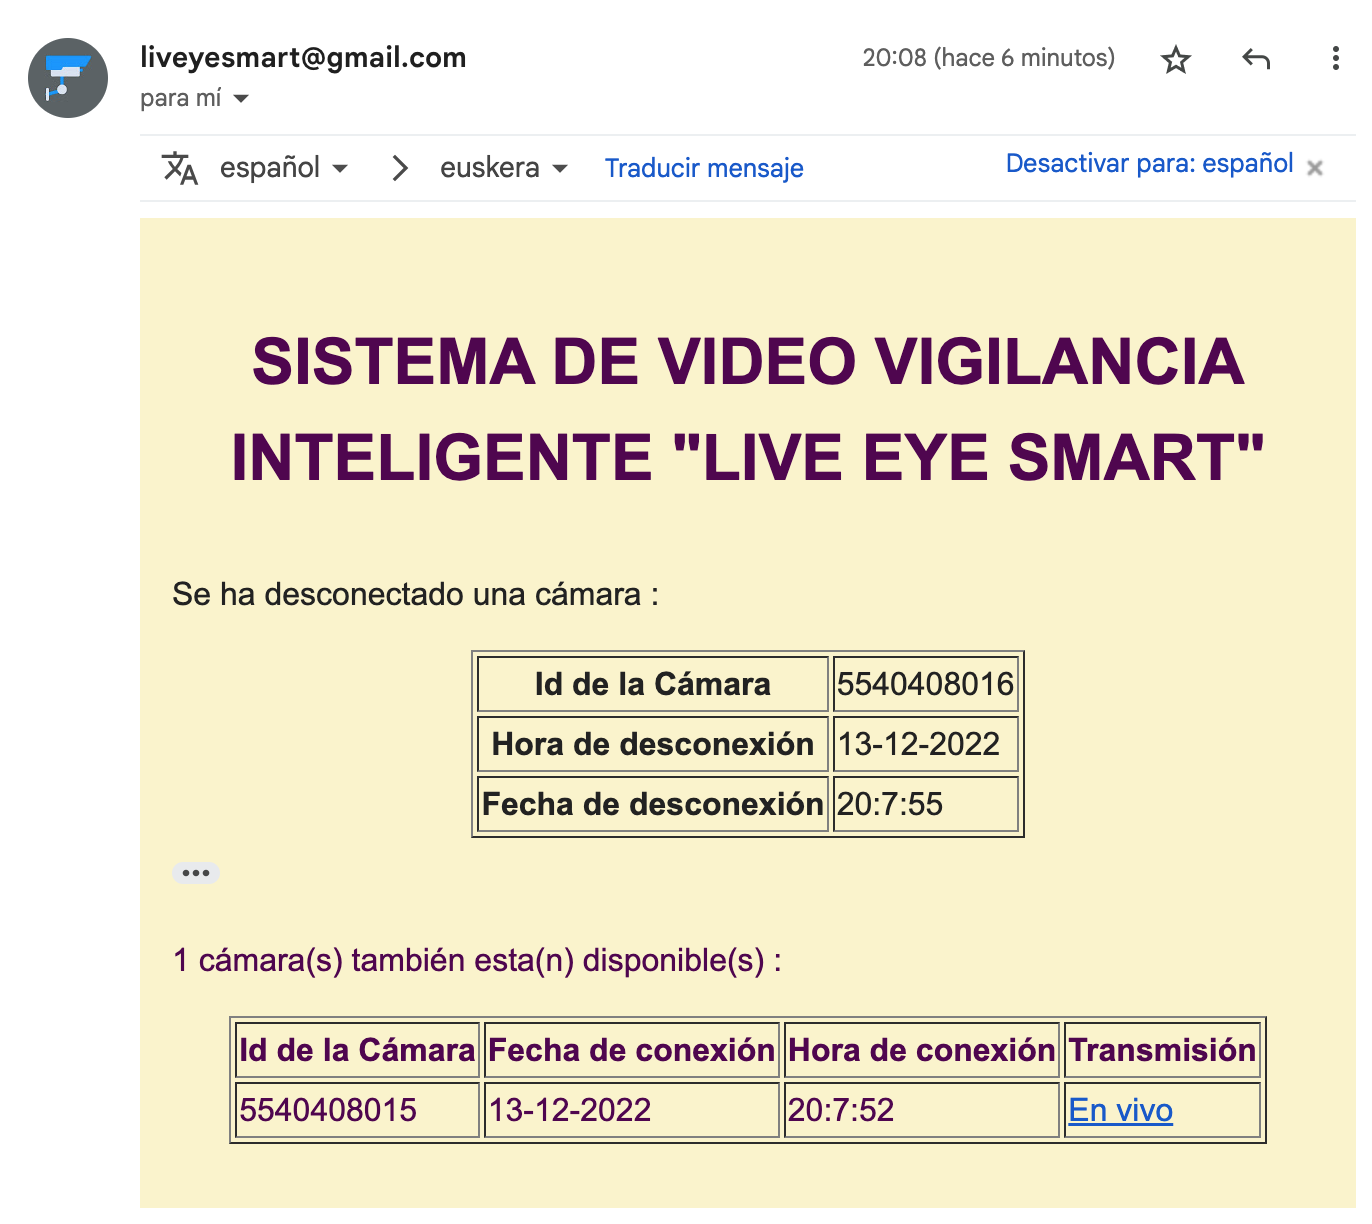
\includegraphics[width=10cm]{img/capitulo_6/mail3.png}
    \end{center}
    \begin{center}
        \caption{Detalle de notificación por correo electrónico.}
        Fuente : Elaboración propia
    \end{center}
\end{figure}

\section{Prueba de detección de fuego y notificación inmediata}

En la siguiente tabla se describe la prueba realizada sobre el detector:\\

\begin{table}[H]
    \caption{Detalle de prueba de detector de fuego}
    \begin{center}
        \begin{tabular}{|>{\centering}p{0.3\textwidth}|m{0.6\textwidth}<{\centering}|} 
            \hline
            \textbf{Título de la prueba} & Detector de fuego identifica incidencia \\
            \hline
            \textbf{Descripción} & El servidor se encuentra en ejecución y el proceso de identificación de fuego detecta una incidencia.\\
            \hline
            \textbf{Comportamiento obtenido} & 
            \begin{itemize}
                \item El servidor captura los fotogramas como prueba de la incidencia.
                \item El servidor notifica al usuario por medio de correo electronico.
                \item La notificación provee información sobre la fecha y hora de la incidencia, compartiendo el enlace para la transmisión en vivo.
            \end{itemize} \\ 
            \hline
            \textbf{Estado de prueba} & Exitoso \\
            \hline
        \end{tabular}
    \end{center}
\end{table}

A continuación se muestra las capturas del comportamiento esperado:

\begin{figure}[H]
    \begin{center}
        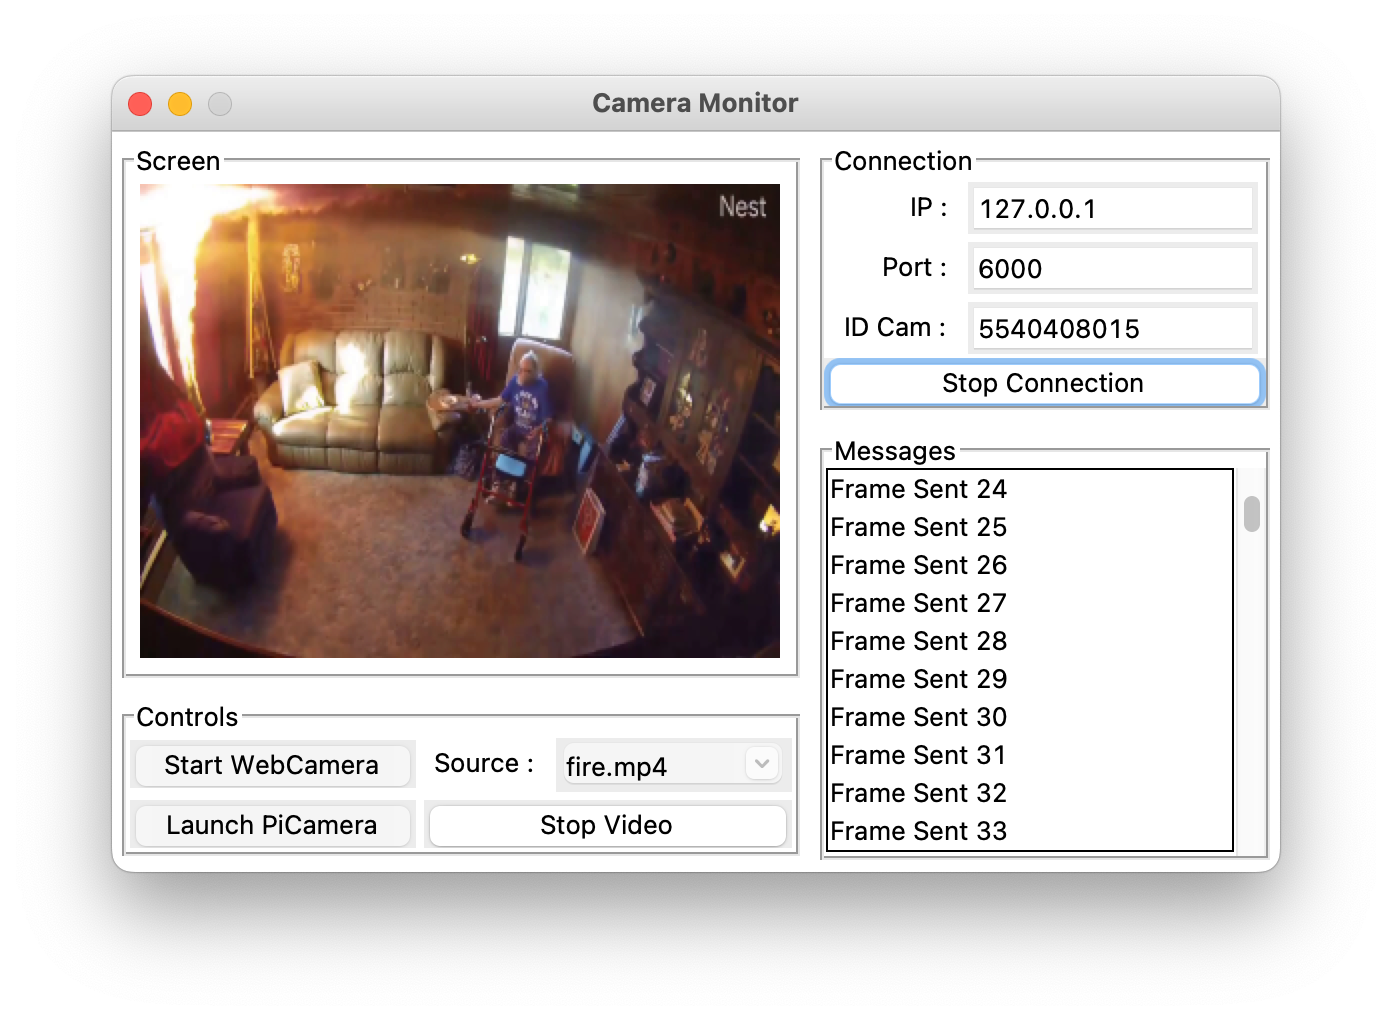
\includegraphics[width=11cm]{img/capitulo_6/fire.png}
    \end{center}
    \begin{center}
        \caption{Mensajes en consola del servidor}
        Fuente : Elaboración propia
    \end{center}
\end{figure}

\begin{figure}[H]
    \begin{center}
        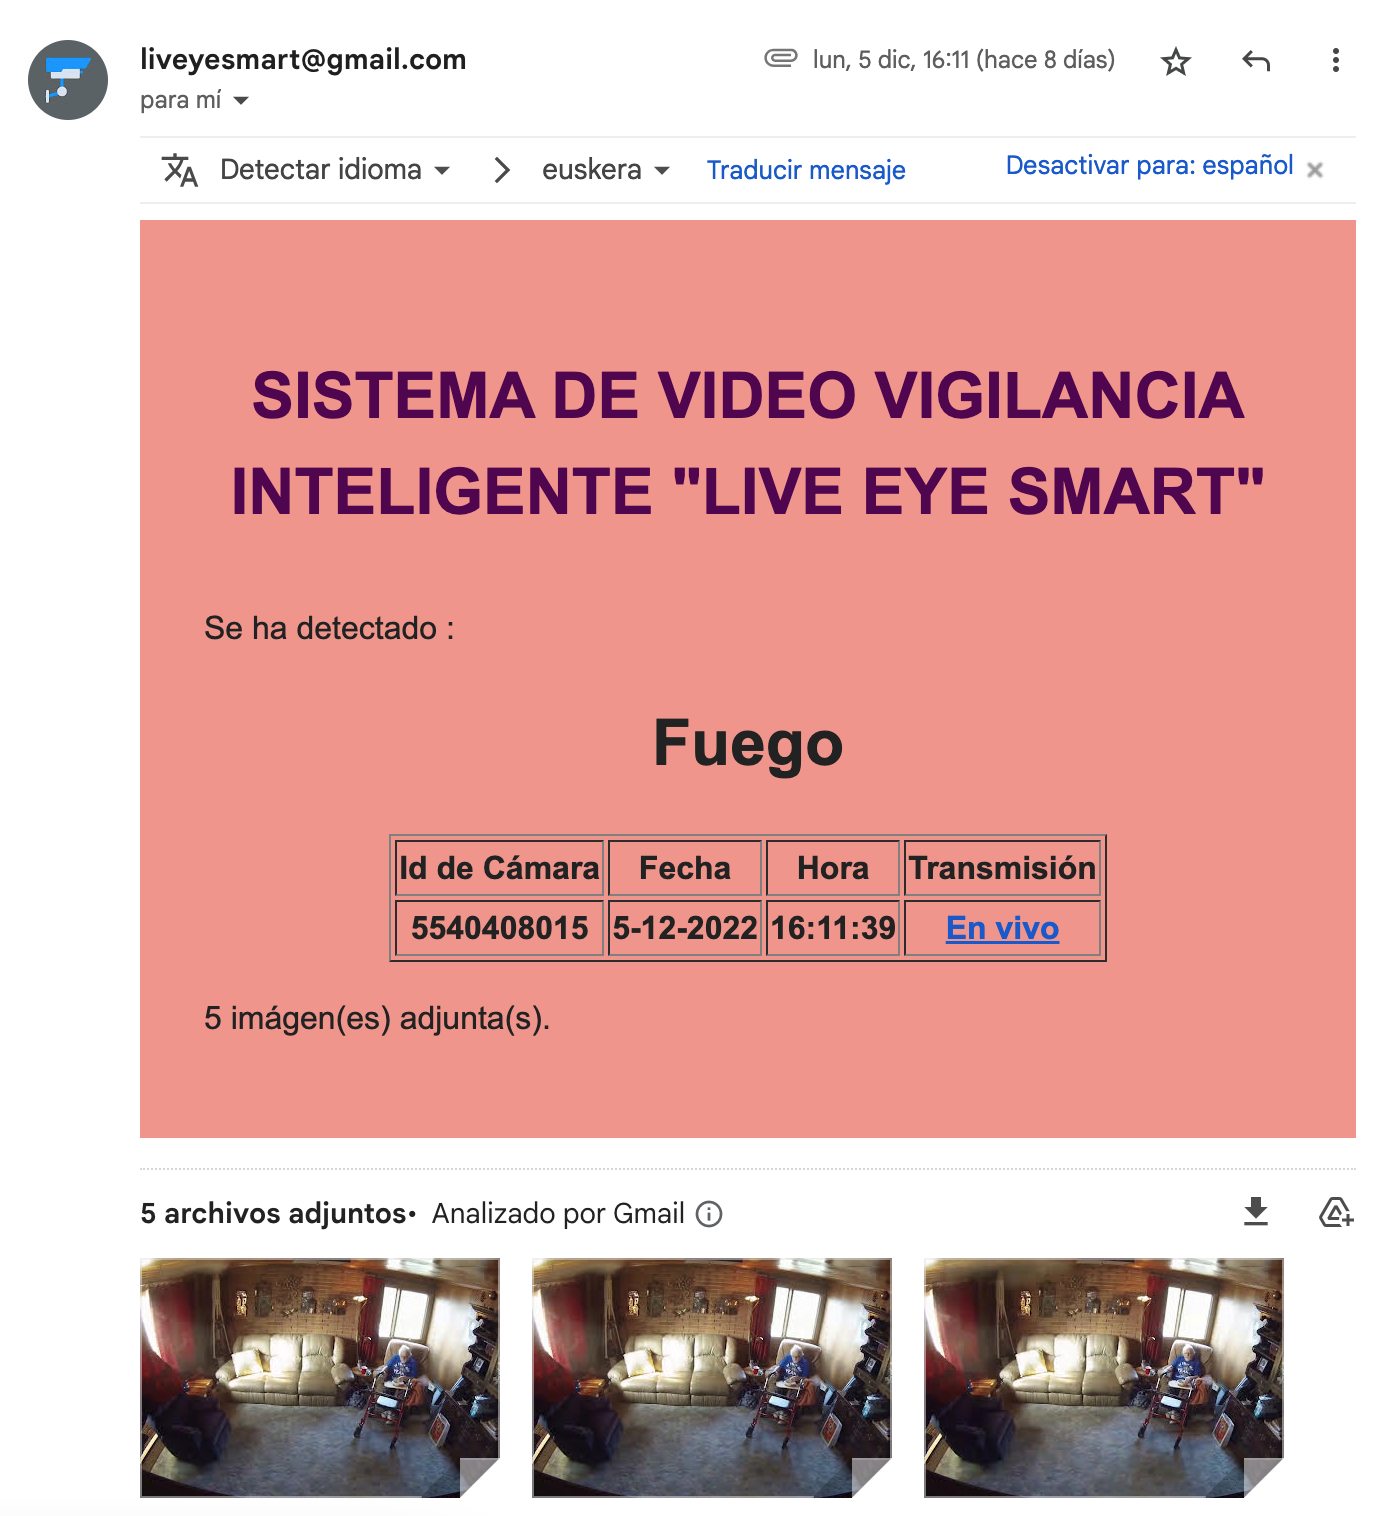
\includegraphics[width=10cm]{img/capitulo_6/mail_fire.png}
    \end{center}
    \begin{center}
        \caption{Detalle de notificación por correo electrónico.}
        Fuente : Elaboración propia
    \end{center}
\end{figure}

\section{Prueba de detección de silueta humana y notificación inmediata}

En la siguiente tabla se describe la prueba realizada sobre el detector:

\begin{table}[H]
    \caption{Detalle de prueba de detector de silueta humana}
    \begin{center}
        \begin{tabular}{|>{\centering}p{0.3\textwidth}|m{0.6\textwidth}<{\centering}|} 
            \hline
            \textbf{Título de la prueba} & Detector de silueta humana identifica incidencia \\
            \hline
            \textbf{Descripción} & El servidor se encuentra en ejecución y el proceso de identificación de silueta humana detecta una incidencia.\\
            \hline
            \textbf{Comportamiento obtenido} & 
            \begin{itemize}
                \item El servidor captura los fotogramas como prueba de la incidencia.
                \item El servidor notifica al usuario por medio de correo electronico.
                \item La notificación provee información sobre la fecha y hora de la incidencia, compartiendo el enlace para la transmisión en vivo.
            \end{itemize} \\ 
            \hline
            \textbf{Estado de prueba} & Exitoso \\
            \hline
        \end{tabular}
    \end{center}
\end{table}

A continuación se muestra las capturas del comportamiento esperado:

\begin{figure}[H]
    \begin{center}
        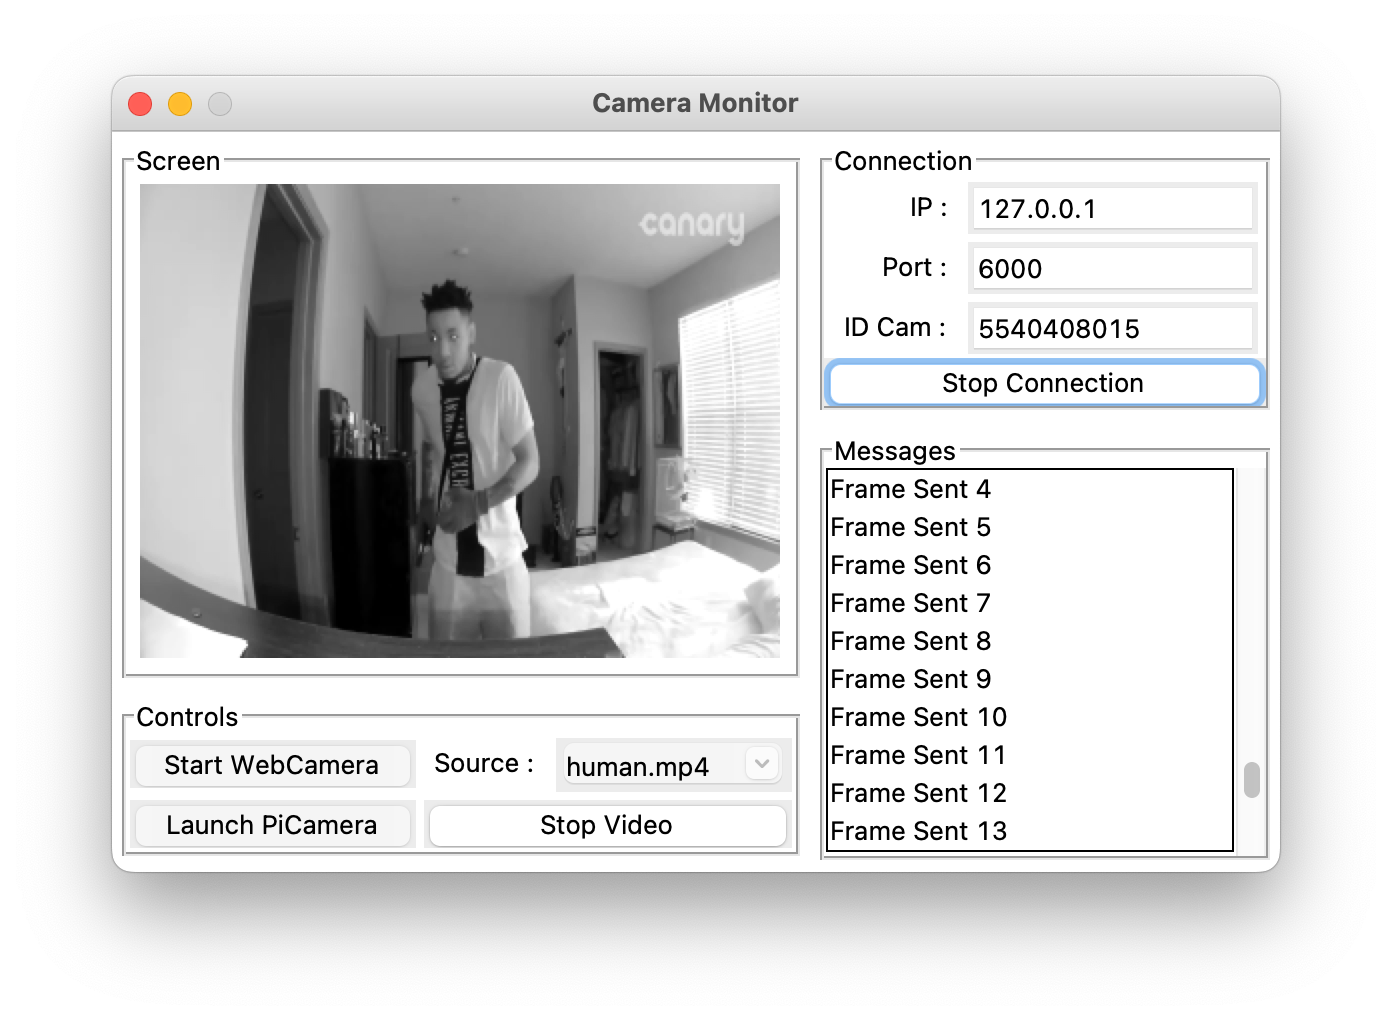
\includegraphics[width=12cm]{img/capitulo_6/human.png}
    \end{center}
    \begin{center}
        \caption{Mensajes en consola del servidor}
        Fuente : Elaboración propia
    \end{center}
\end{figure}

\begin{figure}[H]
    \begin{center}
        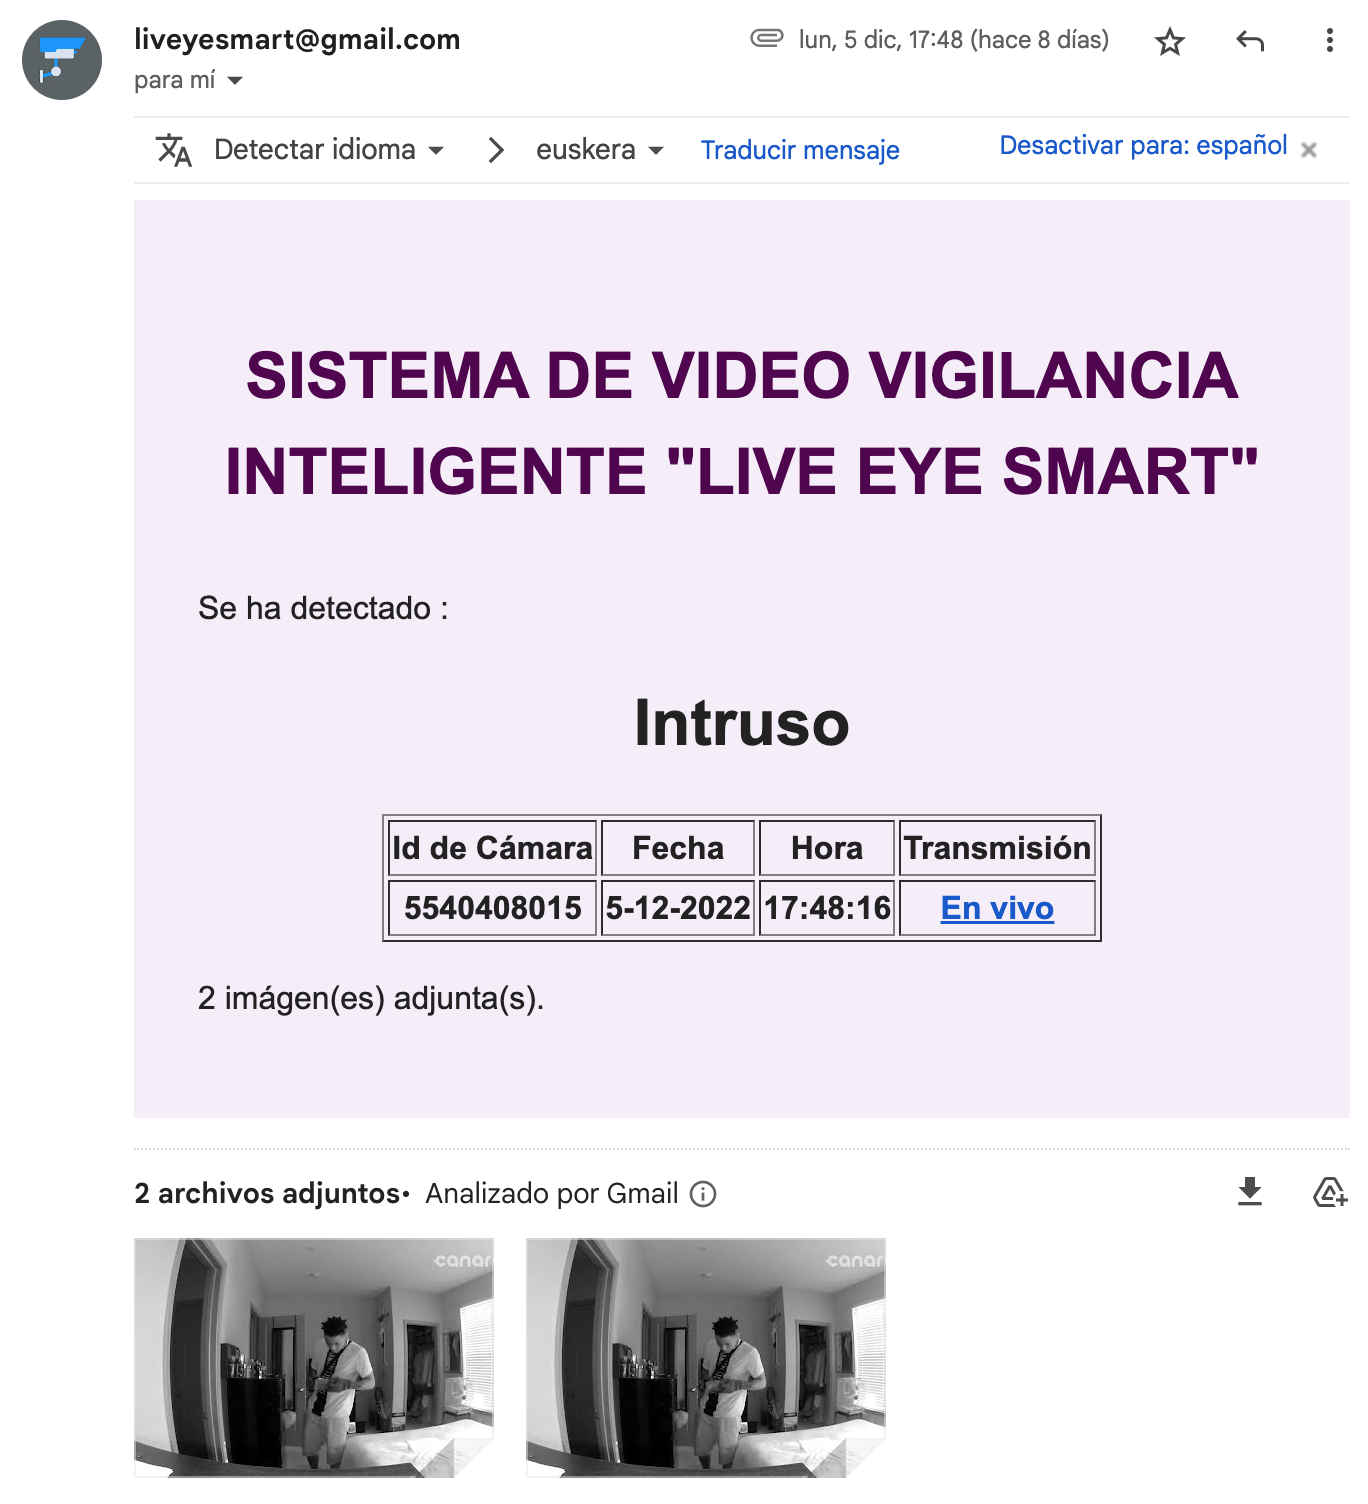
\includegraphics[width=8.8cm]{img/capitulo_6/mail_human.png}
    \end{center}
    \begin{center}
        \caption{Detalle de notificación por correo electrónico.}
        Fuente : Elaboración propia
    \end{center}
\end{figure}


\section{Prueba de detección de movimiento y notificación inmediata}

En la siguiente tabla se describe la prueba realizada sobre el detector:\\

\begin{table}[H]
    \caption{Detalle de prueba de detector de movimiento}
    \begin{center}
        \begin{tabular}{|>{\centering}p{0.3\textwidth}|m{0.6\textwidth}<{\centering}|} 
            \hline
            \textbf{Título de la prueba} & Detector de movimiento identifica incidencia \\
            \hline
            \textbf{Descripción} & El servidor se encuentra en ejecución y el proceso de identificación de silueta humana detecta una incidencia.\\
            \hline
            \textbf{Comportamiento obtenido} & 
            \begin{itemize}
                \item El servidor captura los fotogramas como prueba de la incidencia.
                \item El servidor notifica al usuario por medio de correo electronico.
                \item La notificación provee información sobre la fecha y hora de la incidencia, compartiendo el enlace para la transmisión en vivo.
            \end{itemize} \\ 
            \hline
            \textbf{Estado de prueba} & Exitoso \\
            \hline
        \end{tabular}
    \end{center}
\end{table}

A continuación se muestra las capturas del comportamiento esperado:

\begin{figure}[H]
    \begin{center}
        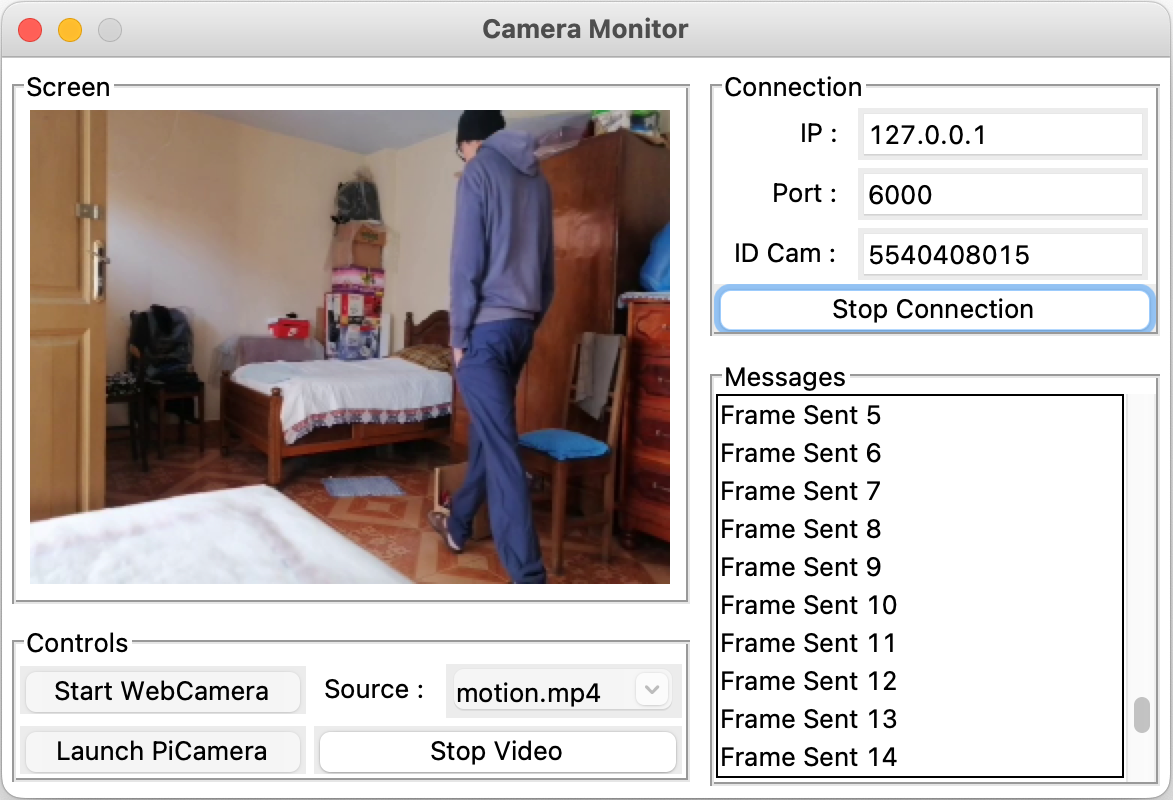
\includegraphics[width=11cm]{img/capitulo_6/motion.png}
    \end{center}
    \begin{center}
        \caption{Mensajes en consola del servidor}
        Fuente : Elaboración propia
    \end{center}
\end{figure}

\begin{figure}[H]
    \begin{center}
        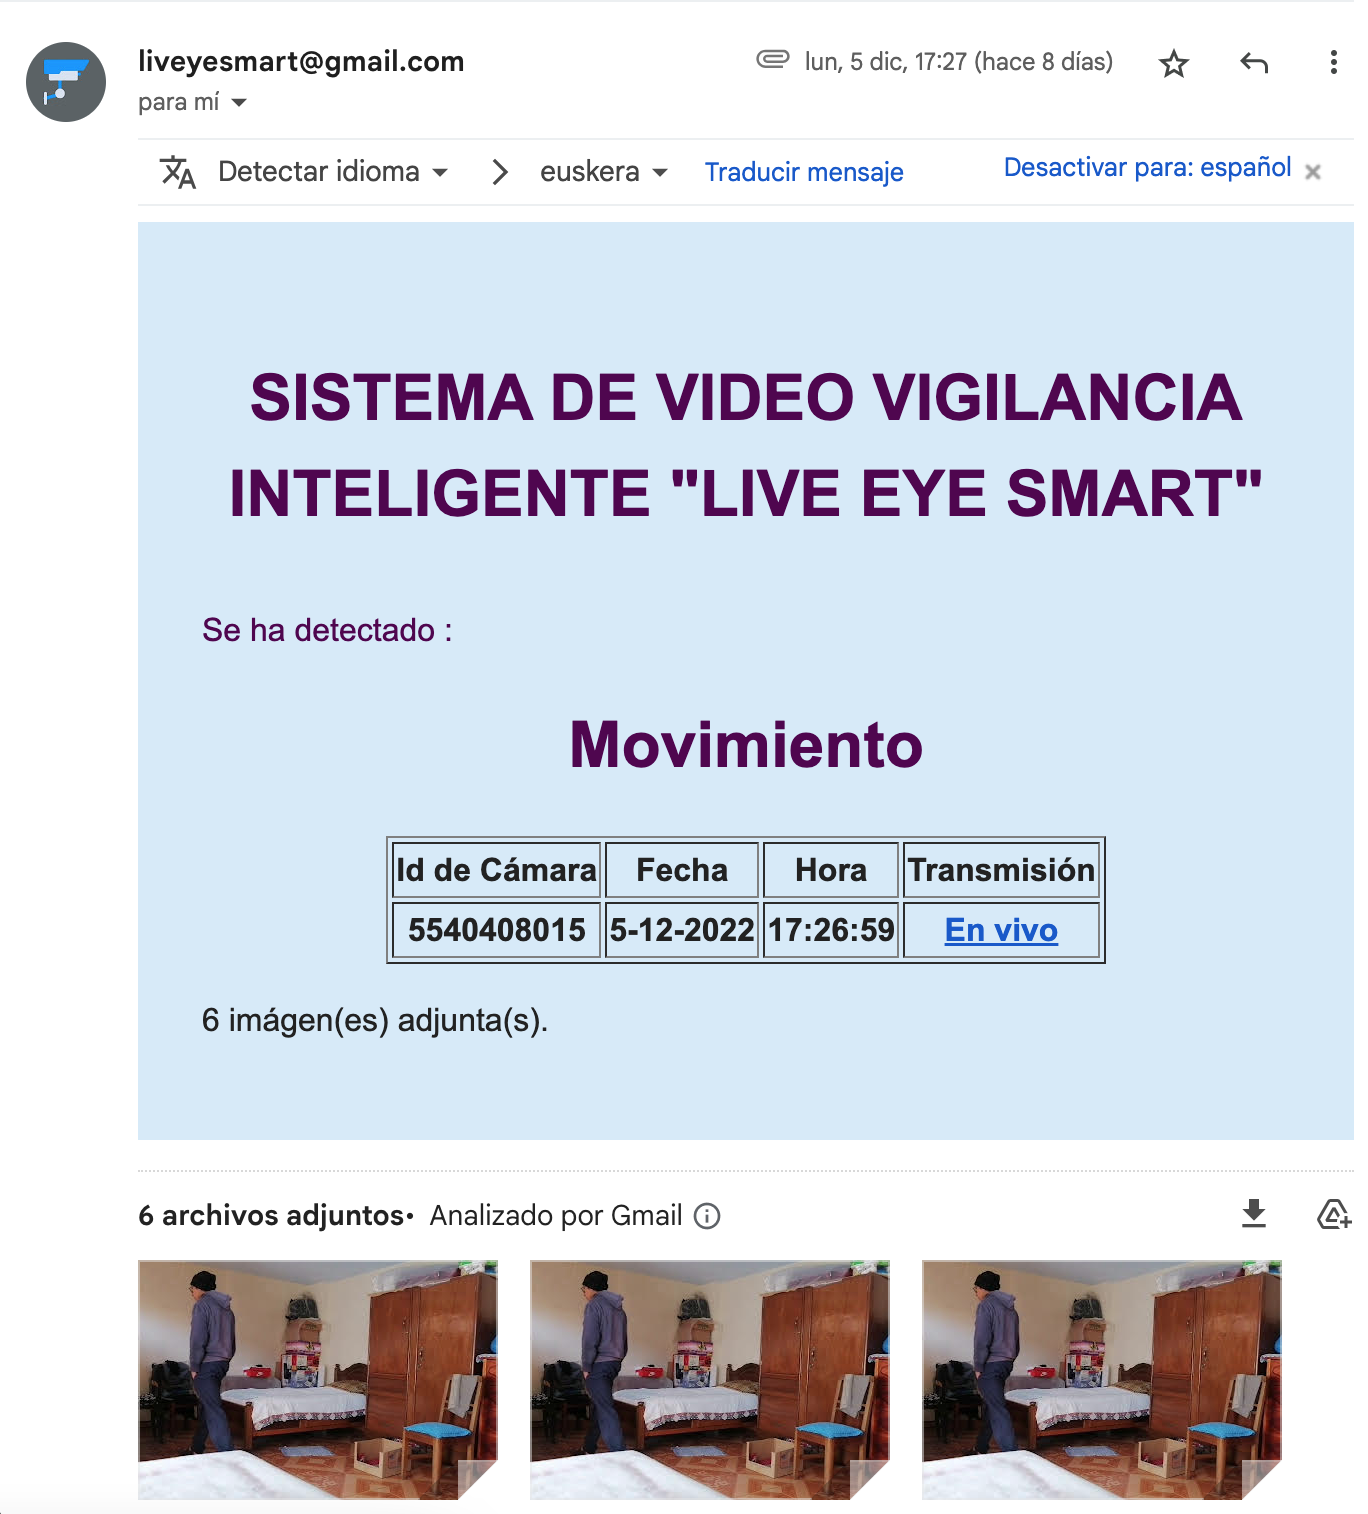
\includegraphics[width=9cm]{img/capitulo_6/mail_motion.png}
    \end{center}
    \begin{center}
        \caption{Detalle de notificación por correo electrónico.}
        Fuente : Elaboración propia
    \end{center}
\end{figure}

\section{Prueba de transmisión de video en vivo}

En la siguiente tabla se describe la prueba realizada:\\

\begin{table}[H]
    \caption{Detalle de prueba de la transmisión de video en vivo.}
    \begin{center}
        \begin{tabular}{|>{\centering}p{0.3\textwidth}|m{0.6\textwidth}<{\centering}|} 
            \hline
            \textbf{Título de la prueba} & Transmisión de video\\
            \hline
            \textbf{Descripción} & El servidor se encuentra en ejecución y una instancia del módulo de cámaras se conecta al servidor. El usuario ingresa al enlace que le llega en la notificación para la transmisión de video en vivo.\\
            \hline
            \textbf{Comportamiento obtenido} & 
            \begin{itemize}
                \item El servidor registra la conexión y lo muestra en consola.
                \item El servidor comienza con la decodificación video en streaming.
                \item La notificación provee información del enlace para su transmisión en vivo.
                \item La transmisión se visualiza en un reproductor de video adaptativo en el navegador.
            \end{itemize} \\ 
            \hline
            \textbf{Estado de prueba} & Exitoso \\
            \hline
        \end{tabular}
    \end{center}
\end{table}

A continuación se muestra las capturas del comportamiento esperado:\\

\begin{figure}[H]
    \begin{center}
        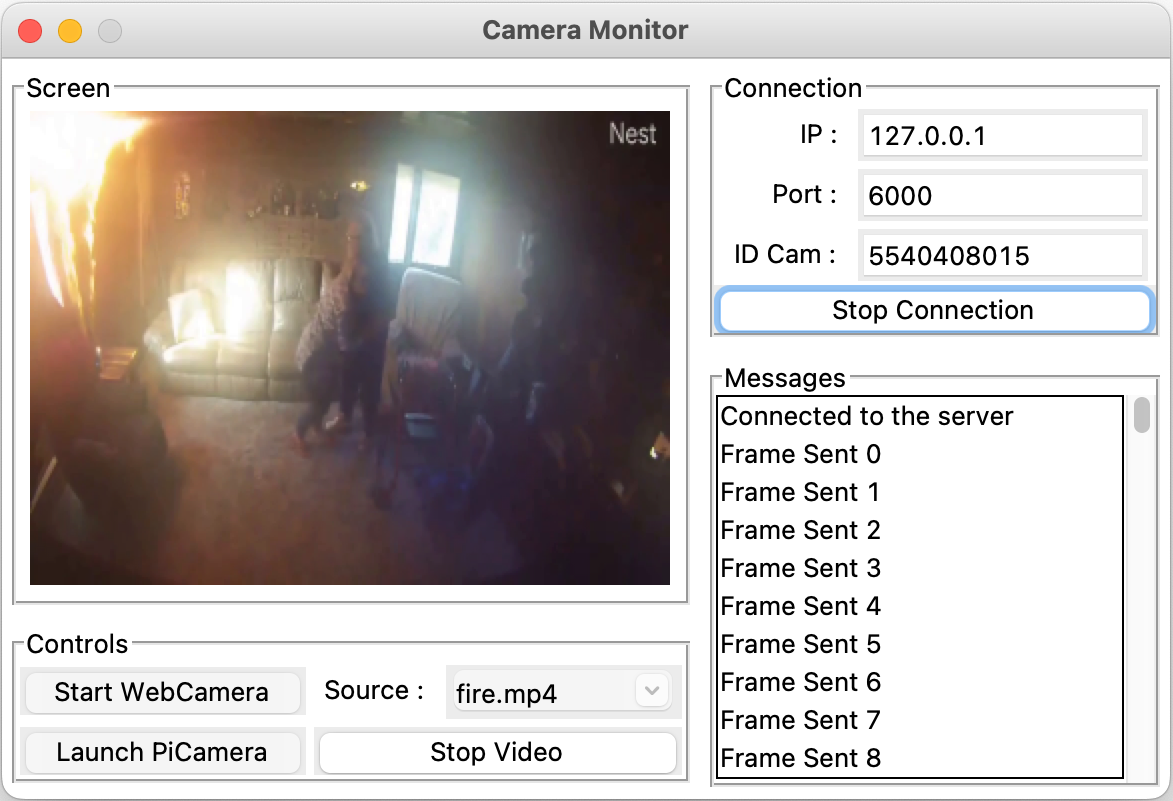
\includegraphics[width=10cm]{img/capitulo_6/stream.png}
        \caption{Mensajes en consola del servidor en parte del}
        Fuente : Elaboración propia
    \end{center}
\end{figure}

\begin{figure}[H]
    \begin{center}
        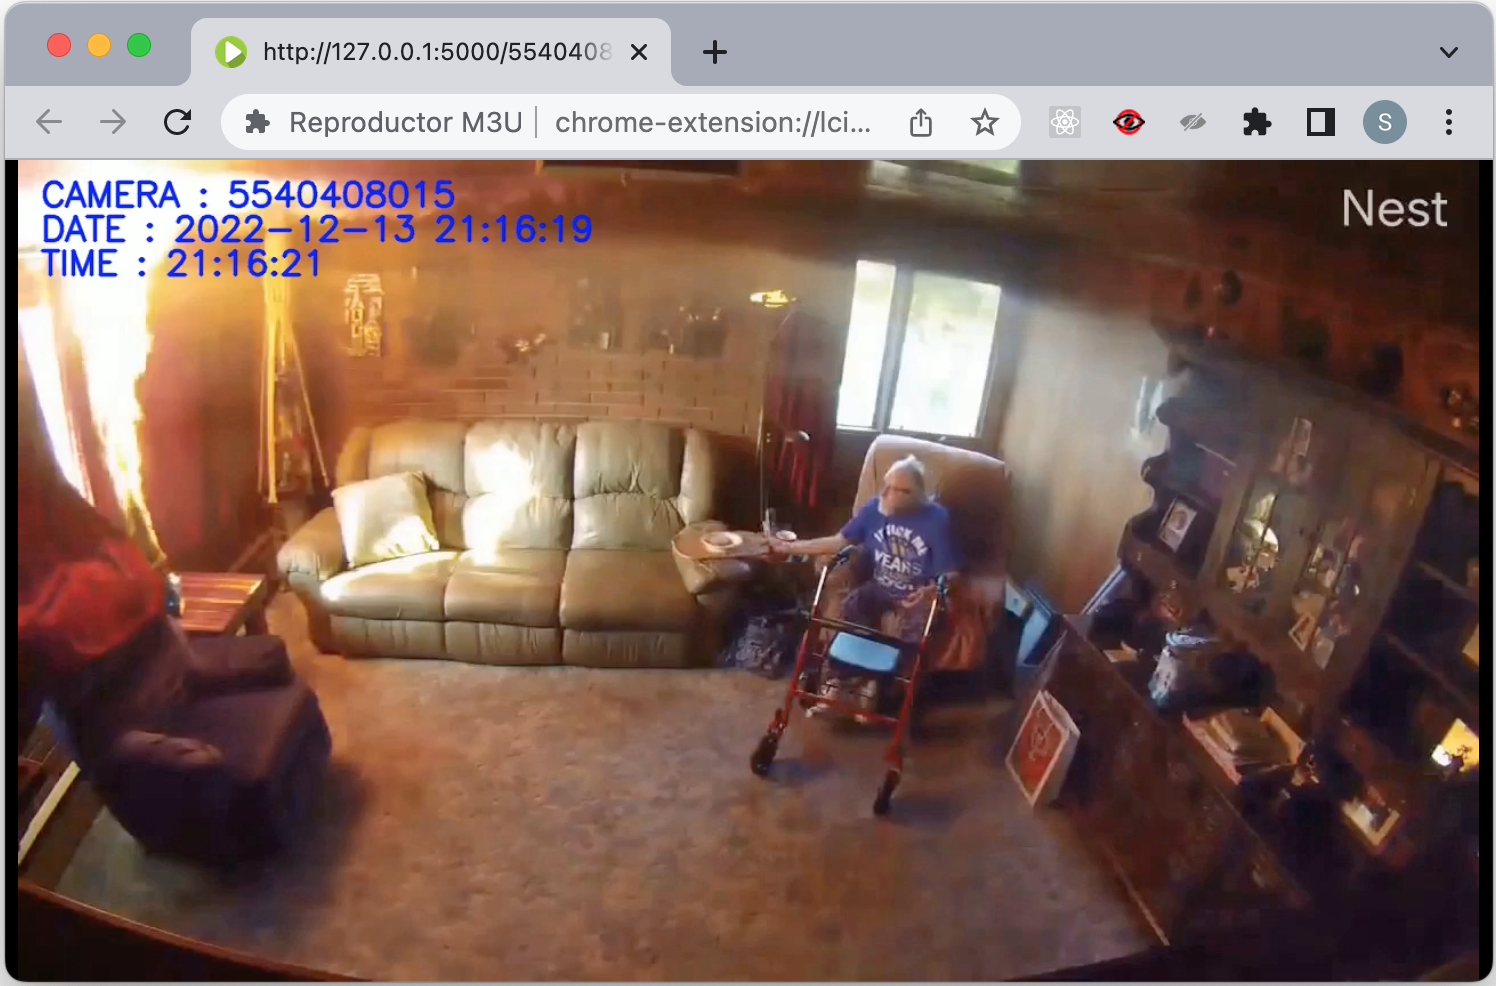
\includegraphics[width=15cm]{img/capitulo_6/stream_web.png}
        \caption{Detalle de notificación por correo electrónico.}
        Fuente : Elaboración propia
    \end{center}
\end{figure}
    \chapter{Conclusiones y Recomendaciones}
\section{Conclusiones}
Las siguientes conclusiones se definen en base a los objetivos específicos planteados en la elaboración del proyecto:\\

\begin{itemize}
    \item La transmisión de datos por la red es el principal medio de comunicación entre sistemas; el desarrollo de diferentes protocolos de red, basados en una arquitectura, ayudaron a proveer usos específicos a las redes de computadoras tanto locales como de Internet. Aplicar los conceptos básicos de la comunicación de sistemas permitio el envio de fotogramas entre los módulos del sistema planteado.
    
    \item La inteligencia artificial y sus diversas ramas proveen de herramientas innovadoras en el campo de la visión por computadora, permitiendo la automatización de tareas de video-vigilancia e industrias, y en general donde es necesaria la supervisión humana.
    
    \item Las redes neuronales son un modelo de aprendizaje artificial que ofrecen identificar caracteristicas a partir de un conjunto de datos generales, de esta manera, permitir la clasificación de la información, facilitando el proceso de automatización. El resultado del entretenimiento de la red neuronal fue útil para el clasificador usado en la detección de fuego.
    
    \item La transmisión de video es una de las aplicaciones de la transmisión de datos por la red, que permiten compartir contenido multimedia para diversos usos tanto para el entretenimiento como para usos industriales y de seguridad. Esta tecnología y el protocolo Http Live Streaming, permitió realizar la transmisión de video en vivo de lo que las cámaras estan capturando.
    
    \item Para el análisis de imágenes es necesario obtener el archivo con el formato correcto; debido a la transmisión de datos por la red, el formato no persiste por lo que es necesario realizar tareas adicionales para poder reconstruir la información recibida y realizar su análisis.
    
    \item El sistema de video-vigilancia inteligente permite automatizar la alerta inmediata ante situaciones de peligro por medio de la notificación por correo electrónico y la visualización de video en vivo.
\end{itemize}

\section{Recomendaciones}
Para finalizar, se recomienda que para escalar el presente proyecto se realize:
\begin{itemize}
    \item Distribuir las tareas de detección en diversos computadores distribuidos en red, para alivianar la carga de los detectores.
    \item Independizar el módulo de transmisión de video en vivo, debido a que es una carga considerable codificar y decodificar video.
    \item Proveer un almacen de imágenes que representan las capturas de cada uno de los detectores.
    \item Implementar una base de datos para guardar un histórico de las detecciónes realizadas.
    \item Implementar una aplicación web para centralizar toda la información según cuentas de usuario. 
\end{itemize}


    % \chapter{Ejemplos}

\section{Mas ejemplos de formato}
\subsection{Familia}

{\ttfamily typewriter (máquina de escribir)}

{\sffamily sans serif}

{\rmfamily roman}

\subsection{Forma}
\textbf{texto en negritas}\\
\textit{texto en itálicas}\\
\textsl{texto inclinado}\\
\texttt{texto en estilo máquina de escribir}\\
\textsc{texto en mayúsculas pequeñas}

\subsection{Tamaño}
{\tiny texto de prueba}\\
{\scriptsize texto de prueba}\\
{\footnotesize texto de prueba}\\
{\small texto de prueba}\\
{\normalsize texto de prueba}\\
{\large texto de prueba}\\
{\Large texto de prueba}\\
{\LARGE texto de prueba}\\
{\huge texto de prueba}\\
{\Huge texto de prueba}

\section{Listado}

\subsection{No numerados}
\begin{itemize}
    \item Item 1
    \item Item 2
    \item Item 3
\end{itemize}

\subsection{Numerados}
\begin{enumerate}
    \item Item 1
    \item Item 2
    \item Item 3
\end{enumerate}


\section{Referenciación con APA}

\subsection{Citación como parte de párrafo}

\subsection*{Un autor}

Como menciona \citeA{libro:ejemplo}, no es la única
forma de citar.\\

\subsection*{Varios autores}

Como menciona \citeA{libro:ejemplo_varios_autores}, no es la única
forma de citar.\\

\subsection{Citación en la parte final}

\subsection*{Un autor}

Duis fringilla tristique neque. Sed interdum libero ut metus.
Pellentesque placerat. Nam rutrum augue a leo. Morbi sed 
elit sit amet ante lobortis sollicitudin.Praesent blandit 
blandit mauris citumoris totalis. \cite{libro:ejemplo}.

\subsection*{Varios autores}

Duis fringilla tristique neque. Sed interdum libero ut metus.
Pellentesque placerat. Nam rutrum augue a leo. Morbi sed 
elit sit amet ante lobortis sollicitudin.Praesent blandit 
blandit mauris citumoris totalis. \cite{libro:ejemplo_varios_autores}.

\subsection{Citación con número de página}

Como menciona \citeA[p.~5]{libro:ejemplo}, no es la única
forma de citar.\\

Duis fringilla tristique neque. Sed interdum libero ut metus.
Pellentesque placerat. Nam rutrum augue a leo. Morbi sed 
elit sit amet ante lobortis sollicitudin.Praesent blandit 
blandit mauris citumoris totalis. \cite[p.~7-12]{libro:ejemplo_varios_autores}.

\subsection{Citación anexos}
Duis fringilla tristique neque. Sed interdum libero ut metus.
Pellentesque placerat (Ver Anexo A).

\section{Figuras}
Referenciando a la figura \ref{fig:ejemplo}.

\begin{figure}[H]
    \begin{center}
        \includegraphics[width=8cm]{img/capitulo_1/figura_ejemplo.png}
    \end{center}
    \caption{Explicación de la figura (Aquí)}
    Fuente: Adaptada de Apellido, N. (2000) \textit{Nombre del libro}.
    Editorial o universidad que lo publicó.
    \label{fig:ejemplo}
\end{figure}

\section{Tablas}

\subsection{Corto}
Referenciando a la tabla \ref{tabla:ejemplo}.\\

\begin{table}[H]
    \caption{Título de la tabla}
    \label{tabla:ejemplo}
    \begin{center}
        \begin{tabular}{c|c|c|c|}
            \cline{2-4}
            & \textbf{Columna 1} & \textbf{Columna 2} & \textbf{Columna 3} \\ \hline
            \multicolumn{1}{|c|}{\textbf{Fila 1}} & item               & item               & item               \\ \hline
            \multicolumn{1}{|c|}{\textbf{Fila 2}} & item               & item               & item               \\ \hline
            \multicolumn{1}{|c|}{\textbf{Fila 3}} & item               & item               & item               \\ \hline
        \end{tabular}
    \end{center}
    Nota. Extraída de Apellido, N. (2000) \textit{Nombre del libro}.
    Editorial o universidad que lo publicó.
\end{table}

\subsection{Multipágina}
Stique neque. Sed interdum libero ut metus.
Pellentesque placerat. Nam rutrum augue a leo. Morbi sed 
elit sit amet ante lobortis sollicitudin.Praesent blandit 
blandit mauris. Praesent lectus tellus, aliquet aliquam,
luctus a, egestas a, turpis.Mauris lacinia lorem sit amet
ipsum. Nunc quis urna dictum turpis accumsan semper. Tabla
\ref{tabla:tabla_largo_ejemplo}.\\

\begin{longtable}{p{2cm}|p{3cm}|p{3cm}|p{3cm}|p{3cm}|}
    \caption{Titulo de tabla multipágina} \label{tabla:tabla_largo_ejemplo} \\
    \cline{2-5}
    \multicolumn{1}{l|}{} & \multicolumn{1}{c|}{\textbf{Columna 1}} & \multicolumn{1}{c|}{\textbf{Columna 2}} & \multicolumn{1}{c|}{\textbf{Columna 3}} & \multicolumn{1}{c|}{\textbf{Columna 4}}\\ \hline
    \endfirsthead

    \multicolumn{5}{c}{{\tablename{} \thetable{} -- Continuación de tabla previa}} \\
    \multicolumn{5}{l}{} \\
    \cline{2-5}
    \multicolumn{1}{l|}{} & \multicolumn{1}{c|}{\textbf{Columna 1}} & \multicolumn{1}{c|}{\textbf{Columna 2}} & \multicolumn{1}{c|}{\textbf{Columna 3}} & \multicolumn{1}{c|}{\textbf{Columna 4}}\\ \hline
    \endhead

    \multicolumn{5}{c}{{Continua en la siguiente página.}} \\
    \endfoot

    \multicolumn{5}{l}{} \\
    \multicolumn{5}{l}{Nota. Extraída de Apellido, N. (2000) \textit{Nombre del libro}. Editorial o universidad que lo publicó.} \\
    \endlastfoot

    \multicolumn{1}{|c|}{\textbf{Fila 1}} & Lorem ipsum dolor sit amet, consectetuer adipiscing elit. & Lorem ipsum dolor sit amet, consectetuer adipiscing elit. & Lorem ipsum dolor sit amet, consectetuer adipiscing elit. & Lorem ipsum dolor sit amet, consectetuer adipiscing elit. \\ \hline
    \multicolumn{1}{|c|}{\textbf{Fila 2}} & Lorem ipsum dolor sit amet, consectetuer adipiscing elit. & Lorem ipsum dolor sit amet, consectetuer adipiscing elit. & Lorem ipsum dolor sit amet, consectetuer adipiscing elit. & Lorem ipsum dolor sit amet, consectetuer adipiscing elit. \\ \hline
    \multicolumn{1}{|c|}{\textbf{Fila 3}} & Lorem ipsum dolor sit amet, consectetuer adipiscing elit. & Lorem ipsum dolor sit amet, consectetuer adipiscing elit. & Lorem ipsum dolor sit amet, consectetuer adipiscing elit. & Lorem ipsum dolor sit amet, consectetuer adipiscing elit. \\ \hline
    \multicolumn{1}{|c|}{\textbf{Fila 4}} & Lorem ipsum dolor sit amet, consectetuer adipiscing elit. & Lorem ipsum dolor sit amet, consectetuer adipiscing elit. & Lorem ipsum dolor sit amet, consectetuer adipiscing elit. & Lorem ipsum dolor sit amet, consectetuer adipiscing elit. \\ \hline
    \multicolumn{1}{|c|}{\textbf{Fila 5}} & Lorem ipsum dolor sit amet, consectetuer adipiscing elit. & Lorem ipsum dolor sit amet, consectetuer adipiscing elit. & Lorem ipsum dolor sit amet, consectetuer adipiscing elit. & Lorem ipsum dolor sit amet, consectetuer adipiscing elit. \\ \hline
    \multicolumn{1}{|c|}{\textbf{Fila 6}} & Lorem ipsum dolor sit amet, consectetuer adipiscing elit. & Lorem ipsum dolor sit amet, consectetuer adipiscing elit. & Lorem ipsum dolor sit amet, consectetuer adipiscing elit. & Lorem ipsum dolor sit amet, consectetuer adipiscing elit. \\ \hline  
    \multicolumn{1}{|c|}{\textbf{Fila 7}} & Lorem ipsum dolor sit amet, consectetuer adipiscing elit. & Lorem ipsum dolor sit amet, consectetuer adipiscing elit. & Lorem ipsum dolor sit amet, consectetuer adipiscing elit. & Lorem ipsum dolor sit amet, consectetuer adipiscing elit. \\ \hline    
    \multicolumn{1}{|c|}{\textbf{Fila 8}} & Lorem ipsum dolor sit amet, consectetuer adipiscing elit. & Lorem ipsum dolor sit amet, consectetuer adipiscing elit. & Lorem ipsum dolor sit amet, consectetuer adipiscing elit. & Lorem ipsum dolor sit amet, consectetuer adipiscing elit. \\ \hline    
    \multicolumn{1}{|c|}{\textbf{Fila 9}} & Lorem ipsum dolor sit amet, consectetuer adipiscing elit. & Lorem ipsum dolor sit amet, consectetuer adipiscing elit. & Lorem ipsum dolor sit amet, consectetuer adipiscing elit. & Lorem ipsum dolor sit amet, consectetuer adipiscing elit. \\ \hline    
    \multicolumn{1}{|c|}{\textbf{Fila 10}} & Lorem ipsum dolor sit amet, consectetuer adipiscing elit. & Lorem ipsum dolor sit amet, consectetuer adipiscing elit. & Lorem ipsum dolor sit amet, consectetuer adipiscing elit. & Lorem ipsum dolor sit amet, consectetuer adipiscing elit. \\ \hline    
    \multicolumn{1}{|c|}{\textbf{Fila 11}} & Lorem ipsum dolor sit amet, consectetuer adipiscing elit. & Lorem ipsum dolor sit amet, consectetuer adipiscing elit. & Lorem ipsum dolor sit amet, consectetuer adipiscing elit. & Lorem ipsum dolor sit amet, consectetuer adipiscing elit. \\ \hline    
    \multicolumn{1}{|c|}{\textbf{Fila 12}} & Lorem ipsum dolor sit amet, consectetuer adipiscing elit. & Lorem ipsum dolor sit amet, consectetuer adipiscing elit. & Lorem ipsum dolor sit amet, consectetuer adipiscing elit. & Lorem ipsum dolor sit amet, consectetuer adipiscing elit. \\ \hline    
\end{longtable}

\section{Fórmulas matemáticas}

\section*{Simple}
\begin{equation}
    e^{i\pi} + 1 = 0
    \label{eq:euler}
\end{equation}

\section*{Matrices}
\begin{equation}
    \left[
    \begin{matrix}
     a & b & c \\
     d & e & f \\
     g & h & i
    \end{matrix}
    \right]
    \label{eq:matriz}
\end{equation}

\section*{Límites}
\begin{equation}
    \lim_{x\rightarrow\infty}\frac{3+x}{x^2} 
    \label{eq:limites}
\end{equation}

\section{Diagramas de flujo}


\begin{center}
    \begin{tikzpicture}[node distance = 3cm, auto]
        \footnotesize
        % Nodos
        \node [block] (init) {Inicio};
        \node [block, below of=init] (test) {Nodo A};
        \node [block, right of=test] (search) {Nodo B};
        \node [decision, below of=test] (test_done) {Decisión A};
        \node [block, below of=test_done] (intregate) {Nodo C};
        \node [cloud, left of=intregate] (code) {Extra};
        \node [decision, below of=intregate] (all_done) {Decisión B};
        \node [block, below of=all_done] (stop) {Nodo D};
        % Cordenadas
        \coordinate[left of=test] (il);
        \coordinate[left of=all_done] (al);
        % Líneas
        \path [line, dashed] (code) -- (intregate);
        \path [line, dashed] (test_done) -| node [near start] {si} (code);
        \path [line] (init) -- (test);
        \path [line] (test) -- (test_done);
        \path [line] (test_done) -- node {si}(intregate);
        \path [line] (test_done) -| node  [near start] {no} (search);
        \path [line] (intregate) -- (all_done);
        \path [line] (all_done.west) |- node [near end] {no} ([xshift=-2.3cm]al) -- ([xshift=-2.3cm]il)-- (test.west);
        \path [line] (all_done) -- node {si} (stop);
        \path [line] (search) -- (test);
    \end{tikzpicture}
\end{center}

\begin{table}[H]
    \caption{Detalle de las pruebas realizadas}
    \begin{center}
        \begin{tabular}{|>{\centering}p{0.6\textwidth}|m{0.3\textwidth}<{\centering}|} 
            \hline
            \textbf{Columna 1} & \textbf{Columna 2} \\
            \hline
            \begin{minipage}{.6\textwidth}
                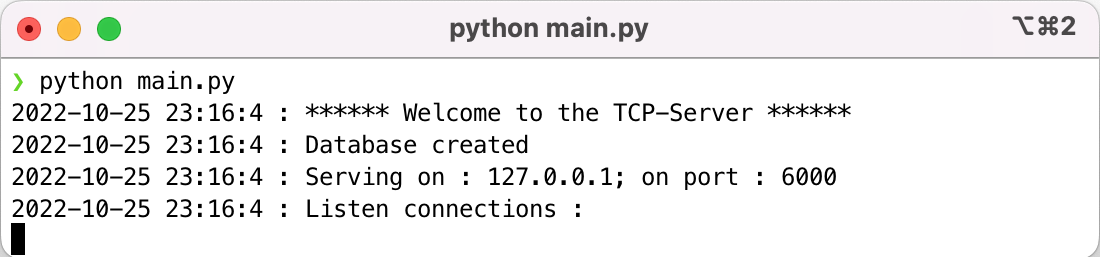
\includegraphics[width=\linewidth]{img/capitulo_5/tcp_server.png}
            \end{minipage}
            & 
            \begin{itemize} 
                \item Remote delivery 
                \item Immersive experiences
                \item text proved
            \end{itemize} \\ 
            \hline
            \begin{minipage}{0.6\textwidth}
                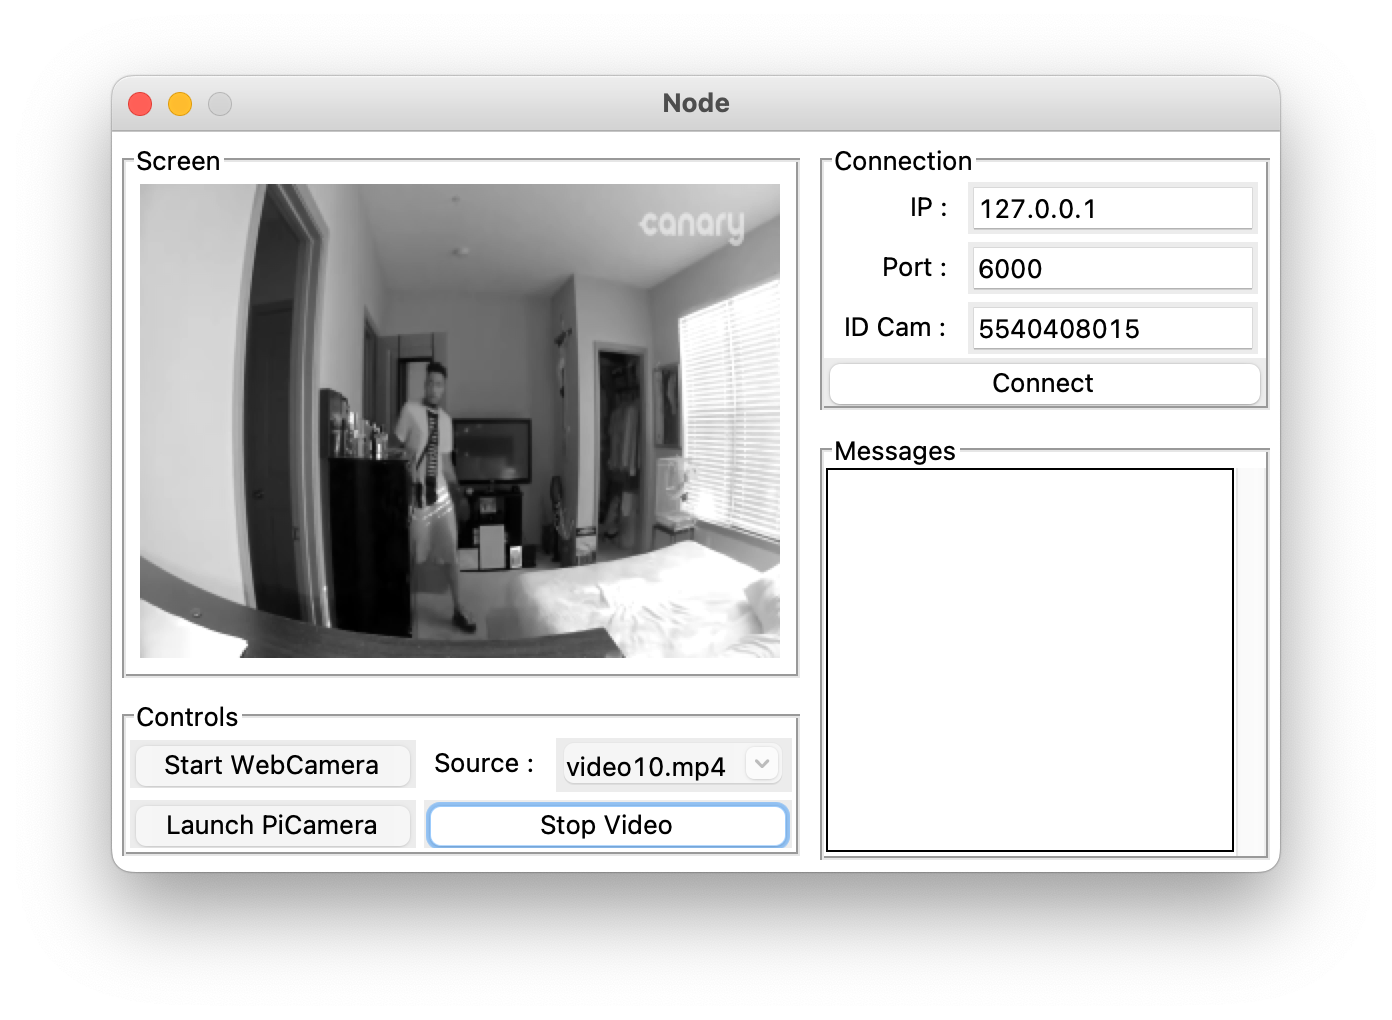
\includegraphics[width=\linewidth]{img/capitulo_5/security-video.png}
            \end{minipage} 
            & 
            \begin{itemize} 
                \item Remote delivery 
                \item Immersive experiences
                \item text proved
            \end{itemize} \\
            \hline
        \end{tabular}
    \end{center}
\end{table}


\begin{table}[H]
    \caption{Detalle de las pruebas realizadas}
    \label{tabla:ejemplo}
    \begin{center}
        \begin{tabular}{c|c|c|c|}
            \cline{2-4}
            & \textbf{Columna 1} & \textbf{Columna 2} & \textbf{Columna 3} \\ \hline
            \multicolumn{1}{|c|}{Fila 1 }& item             & item               & item               \\ \hline
            \multicolumn{1}{|c|} {Fila 2} & {item}               & item               & item               \\ \hline
            \multicolumn{1}{|c|} {Fila 3} & {item}              & item               & item               \\  \hline
        \end{tabular}
    \end{center}
    Nota. Extraída de Apellido, N. (2000) \textit{Nombre del libro}.
    Editorial o universidad que lo publicó.
\end{table}

% \begin{longtable}{p{2cm}|p{3cm}|p{3cm}|p{3cm}|p{3cm}|}
%     \caption{Titulo de tabla multipágina} \label{tabla:tabla_largo_ejemplo} \\
%     \cline{2-5}
%     \multicolumn{1}{l|}{} & \multicolumn{1}{c|}{\textbf{Columna 1}} & \multicolumn{1}{c|}{\textbf{Columna 2}} & \multicolumn{1}{c|}{\textbf{Columna 3}} & \multicolumn{1}{c|}{\textbf{Columna 4}}\\ \hline
%     \endfirsthead

%     \multicolumn{5}{c}{{\tablename{} \thetable{} -- Continuación de tabla previa}} \\
%     \multicolumn{5}{l}{} \\
%     \cline{2-5}
%     \multicolumn{1}{l|}{} & \multicolumn{1}{c|}{\textbf{Columna 1}} & \multicolumn{1}{c|}{\textbf{Columna 2}} & \multicolumn{1}{c|}{\textbf{Columna 3}} & \multicolumn{1}{c|}{\textbf{Columna 4}}\\ \hline
%     \endhead

%     \multicolumn{5}{c}{{Continua en la siguiente página.}} \\
%     \endfoot

%     \multicolumn{5}{l}{} \\
%     \multicolumn{5}{l}{Nota. Extraída de Apellido, N. (2000) \textit{Nombre del libro}. Editorial o universidad que lo publicó.} \\
%     \endlastfoot

%     \multicolumn{1}{|c|}{\textbf{Fila 1}} & Lorem ipsum dolor sit amet, consectetuer adipiscing elit. & Lorem ipsum dolor sit amet, consectetuer adipiscing elit. & Lorem ipsum dolor sit amet, consectetuer adipiscing elit. & Lorem ipsum dolor sit amet, consectetuer adipiscing elit. \\ \hline
%     \multicolumn{1}{|c|}{\textbf{Fila 2}} & Lorem ipsum dolor sit amet, consectetuer adipiscing elit. & Lorem ipsum dolor sit amet, consectetuer adipiscing elit. & Lorem ipsum dolor sit amet, consectetuer adipiscing elit. & Lorem ipsum dolor sit amet, consectetuer adipiscing elit. \\ \hline
%     \multicolumn{1}{|c|}{\textbf{Fila 3}} & Lorem ipsum dolor sit amet, consectetuer adipiscing elit. & Lorem ipsum dolor sit amet, consectetuer adipiscing elit. & Lorem ipsum dolor sit amet, consectetuer adipiscing elit. & Lorem ipsum dolor sit amet, consectetuer adipiscing elit. \\ \hline
%     \multicolumn{1}{|c|}{\textbf{Fila 4}} & Lorem ipsum dolor sit amet, consectetuer adipiscing elit. & Lorem ipsum dolor sit amet, consectetuer adipiscing elit. & Lorem ipsum dolor sit amet, consectetuer adipiscing elit. & Lorem ipsum dolor sit amet, consectetuer adipiscing elit. \\ \hline
%     \multicolumn{1}{|c|}{\textbf{Fila 5}} & Lorem ipsum dolor sit amet, consectetuer adipiscing elit. & Lorem ipsum dolor sit amet, consectetuer adipiscing elit. & Lorem ipsum dolor sit amet, consectetuer adipiscing elit. & Lorem ipsum dolor sit amet, consectetuer adipiscing elit. \\ \hline
%     \multicolumn{1}{|c|}{\textbf{Fila 6}} & Lorem ipsum dolor sit amet, consectetuer adipiscing elit. & Lorem ipsum dolor sit amet, consectetuer adipiscing elit. & Lorem ipsum dolor sit amet, consectetuer adipiscing elit. & Lorem ipsum dolor sit amet, consectetuer adipiscing elit. \\ \hline  
%     \multicolumn{1}{|c|}{\textbf{Fila 7}} & Lorem ipsum dolor sit amet, consectetuer adipiscing elit. & Lorem ipsum dolor sit amet, consectetuer adipiscing elit. & Lorem ipsum dolor sit amet, consectetuer adipiscing elit. & Lorem ipsum dolor sit amet, consectetuer adipiscing elit. \\ \hline    
%     \multicolumn{1}{|c|}{\textbf{Fila 8}} & Lorem ipsum dolor sit amet, consectetuer adipiscing elit. & Lorem ipsum dolor sit amet, consectetuer adipiscing elit. & Lorem ipsum dolor sit amet, consectetuer adipiscing elit. & Lorem ipsum dolor sit amet, consectetuer adipiscing elit. \\ \hline    
%     \multicolumn{1}{|c|}{\textbf{Fila 9}} & Lorem ipsum dolor sit amet, consectetuer adipiscing elit. & Lorem ipsum dolor sit amet, consectetuer adipiscing elit. & Lorem ipsum dolor sit amet, consectetuer adipiscing elit. & Lorem ipsum dolor sit amet, consectetuer adipiscing elit. \\ \hline    
%     \multicolumn{1}{|c|}{\textbf{Fila 10}} & Lorem ipsum dolor sit amet, consectetuer adipiscing elit. & Lorem ipsum dolor sit amet, consectetuer adipiscing elit. & Lorem ipsum dolor sit amet, consectetuer adipiscing elit. & Lorem ipsum dolor sit amet, consectetuer adipiscing elit. \\ \hline    
%     \multicolumn{1}{|c|}{\textbf{Fila 11}} & Lorem ipsum dolor sit amet, consectetuer adipiscing elit. & Lorem ipsum dolor sit amet, consectetuer adipiscing elit. & Lorem ipsum dolor sit amet, consectetuer adipiscing elit. & Lorem ipsum dolor sit amet, consectetuer adipiscing elit. \\ \hline    
%     \multicolumn{1}{|c|}{\textbf{Fila 12}} & Lorem ipsum dolor sit amet, consectetuer adipiscing elit. & Lorem ipsum dolor sit amet, consectetuer adipiscing elit. & Lorem ipsum dolor sit amet, consectetuer adipiscing elit. & Lorem ipsum dolor sit amet, consectetuer adipiscing elit. \\ \hline    
% \end{longtable}

\begin{center}
    \begin{tabular}{ |c|c|c|c| } 
    \hline
    \textbf{col1} & \textbf{col2} & \textbf{col3} \\
    \hline
    \multirow{3}{4em}{Multiple row} & cell2 & cell3 \\ 
    & cell5 & cell6  \\
    & cell8 & cell9 \\ 
    \hline
    \end{tabular}
\end{center}


    \backmatter
    \bibliographystyle{apacite}
    \bibliography{bibliografia}

    \appendix
    \clearpage
    \addappheadtotoc
    \appendixpage
    \chapter{Anexo A: Manual de instalación}

A continuación se detallan los pasos a seguir para el despliegue del sistema de video-vigilancia inteligente. Para la instalación general es necesario tener instalado en el equipo los siguientes paquetes de software:

\begin{enumerate}
    \item Python (Version 3.7 o posterior).
    \item venv (Manejador de entornos virtuales)
    \item git (Controlador de versiones)
    \item pip (Manejador de paquetes de python) 
\end{enumerate}

Por otra parte, el dispositivo donde se realizará la instalación debe contar con una conexión a la red de internet.

\section*{Módulo de cámaras}
Este módulo puede ser instalado en un computador (laptop o de escritorio) como también en un dispositivo RaspberryPi, el cual debe tener previamente instalados los paquetes requeridos anteriormente descritos. Este módulo permite la conexión de una cámara web (integrada o individual) al servidor del sistema de video-vigilancia, por lo que es necesario contar con una.\\

Para realizar la instalación del módulo de cámaras se siguen los siguientes pasos:

\begin{enumerate}
    \item Descargar el código fuente de la aplicación desde el enlace: \begin{center}
        \url{https://github.com/srodrigo23/security-camera.git}
    \end{center}
    \item En el directorio de la carpeta de descarga, se debe crear el entorno virtual del módulo por medio del siguiente comando: 
    \begin{center}
        \shellcmd{python3 -m venv .venv}    
    \end{center}
    \item Instalar las depencias del módulo por medio del comando:
    \begin{center}
        \shellcmd{pip install -r requirements.txt}
    \end{center} 
    \item Una vez instaladas las depencias solo queda lanzar la ejecución del módulo por medio del comando:\begin{center}
        \shellcmd{./run.sh}
    \end{center}
\end{enumerate}

Una vez completados los pasos se carga la vista del módulo de cámaras, listo para su conexión con el servidor.

\begin{figure}[H]
    \begin{center}
        \includegraphics[width=13cm]{img/anexos/mod_camera.png}
        \caption{Interfaz del módulo de cámaras.}
        Fuente : Elaboración propia
    \end{center}
\end{figure}

\section*{Módulo de servidor}
El módulo de servidor consta de dos sub-módulos: servidor-TCP y el servidor-WEB. Ambos son relevantes para el sistema de video-vigilancia, por lo cual deben estar correctamente instalados para una correcta ejecución del sistema.
\subsection*{Servidor TCP}
Este módulo puede ser instalado en un computador (laptop o de escritorio). Durante su ejecución espera nuevas conexiones del módulo de cámaras, para gestionar la transmisión de fotogramas, realizar las detecciones y mandar las notificaciones.\\

Para realizar la instalación del módulo del servidor-TCP se siguen los siguientes pasos:
\begin{enumerate}
    \item Descargar el código fuente de la aplicación desde el enlace: \begin{center}
        \url{https://github.com/srodrigo23/security-system-server.git}
    \end{center}
    \item En el directorio de la carpeta de descarga, se debe crear el entorno virtual del módulo por medio del siguiente comando: 
    \begin{center}
        \shellcmd{python3 -m venv .venv}    
    \end{center}
    \item Instalar las depencias del módulo por medio del comando:
    \begin{center}
        \shellcmd{pip install -r requirements.txt}
    \end{center} 
    \item Una vez instaladas las depencias solo queda lanzar la ejecución del módulo por medio del comando:\begin{center}
        \shellcmd{./run.sh}
    \end{center}
\end{enumerate}

Una vez completados los pasos se carga la interfaz de consola del servidor-TCP, listo para recibir conexiones de cámaras.

\begin{figure}[H]
    \begin{center}
        \includegraphics[width=13cm]{img/anexos/mod_tcp.png}
        \caption{Interfaz de consola del servidor TCP.}
        Fuente : Elaboración propia
    \end{center}
\end{figure}
\subsection*{Servidor web}

Este módulo puede ser instalado en un computador (laptop o de escritorio) como también en un dispositivo RaspberryPi, el cual debe tener previamente instalados los paquetes requeridos anteriormente descritos. Este gestionar las solicitudes HTTP que provienen desde un reprodicutor web de video adaptativo permitiendo asi la transmisión de video en vivo.\\

Para realizar la instalación del servidor web se deben seguir los siguientes pasos:

\begin{enumerate}
    \item Descargar el código fuente de la aplicación desde el enlace: \begin{center}
        \url{https://github.com/srodrigo23/webserver.git}
    \end{center}
    \item En el directorio de la carpeta de descarga, se debe crear el entorno virtual del módulo por medio del siguiente comando: 
    \begin{center}
        \shellcmd{python3 -m venv .venv}    
    \end{center}
    \item Instalar las depencias del módulo por medio del comando:
    \begin{center}
        \shellcmd{pip install -r requirements.txt}
    \end{center} 
    \item Una vez instaladas las depencias solo queda lanzar la ejecución del módulo por medio del comando:\begin{center}
        \shellcmd{./run.sh}
    \end{center}
\end{enumerate}

Una vez completados los pasos se carga interfaz de consola del servidor-WEB, listo para atender todas las peticiones HTTP al servidor.

\begin{figure}[H]
    \begin{center}
        \includegraphics[width=13cm]{img/anexos/mod_web.png}
        \caption{Interfaz de consola del servidor Web.}
        Fuente : Elaboración propia
    \end{center}
\end{figure}

    \chapter{Anexo B: Manual de Usuario}

La mayoria de las tareas que realiza este sistema de video-vigilancia inteligente son automáticas, pero las tareas más basicas a describir son las siguientes:

% \begin{enumerate}
%     \item Conectar cámara
%     \item Desconectar cámara
%     \item Recibir notificaciones
% \end{enumerate}
\section*{Conectar cámara}
Para conectar una nueva cámara es necesario tener el servidor-TCP funcionando. Para levantas una nueva instancia de cámara se siguen los siguientes pasos:
\begin{enumerate}
    \item En el directorio donde se desplego el módulo de cámaras ejecutar el siguiente comando:\begin{center}
        \shellcmd{./run.sh}
    \end{center}
    \item De acuerdo a la configuración del servidor-TCP ingrerar los valores de dirección y puerto en el formato siguiente:
    \begin{itemize}
        \item Dirección : 0.0.0.0 hasta 255.2555.255.2555
        \item Puerto: Desde 49152 hasta 65535
        \item ID Cam: valor numérico para el identificador
    \end{itemize}
    Definir estos valores en los campos correspondientes:
    \begin{figure}[H]
        \begin{center}
            \includegraphics[width=5cm]{img/anexos/ip_port.png}
            % \caption{Interfaz del módulo de cámaras.}
            % Fuente : Elaboración propia
        \end{center}
    \end{figure}
    
    \item En el panel de controles se tiene 3 opciones para iniciar el módulo antes de conectarse:
        \begin{itemize}
            \item[A]: Iniciar cámara web integrada o externa.
            \item[B]: Iniciar PiCámara, solo si esta disponible en un equipo RaspberryPi.
            \item[C]: Iniciar Video, en caso de solo contar con grabaciones.  
        \end{itemize}
    \begin{figure}[H]
        \begin{center}
            \includegraphics[width=10cm]{img/anexos/controls_camera.png}
            % \caption{Interfaz del módulo de cámaras.}
            % Fuente : Elaboración propia
        \end{center}
    \end{figure}
    Se elige una de esas opciones según al requerimientos del usuario.
    \item Presionar el boton ``Conectar'' y se empezará a enviar los fotogramas de video.
    \begin{center}
        \includegraphics[width=10cm]{img/anexos/send_frames.png}
        % \caption{Interfaz del módulo de cámaras.}
        % Fuente : Elaboración propia
    \end{center}
    
\end{enumerate}

\section*{Desconectar cámara}

Cuando se tiene una cámara ejecutando el envio de fotogramas, es posible que el usuario quiera desconectarlo. Para este objetivo se siguen los siguientes pasos.
\begin{enumerate}
    \item Parar la conección presionando en el botón: ``Stop Connection''.
    \begin{center}
        \includegraphics[width=5cm]{img/anexos/stop_connection.png}
        % \caption{Interfaz del módulo de cámaras.}
        % Fuente : Elaboración propia
    \end{center}
    \item En caso de querer apagar la cámara se debera presionar en su debido botón la opcion de ``Parar Cámara''
    \begin{center}
        \includegraphics[width=10cm]{img/anexos/stop_video.png}
        % \caption{Interfaz del módulo de cámaras.}
        % Fuente : Elaboración propia
    \end{center}
\end{enumerate}

\section*{Visualizar transmisión de video en vivo}
Para la visualización del video en vivo se recibe un correo eléctrónico con el enlace directo a la transmisión.

Para reproducir esta transmisión se debe seguir los siguientes pasos:
\begin{enumerate}
    \item Revisar el correo electrónico correspodiente a la conexión.
    \begin{center}
        \includegraphics[width=10cm]{img/anexos/link.png}
        % \caption{Interfaz del módulo de cámaras.}
        % Fuente : Elaboración propia
    \end{center}
    \item Redirigirse al enlace de transmisión.
    \begin{center}
        \includegraphics[width=10cm]{img/anexos/stream_web.png}
        % \caption{Interfaz del módulo de cámaras.}
        % Fuente : Elaboración propia
    \end{center}
\end{enumerate}
    \chapter{Anexo C: Instalación de la aplicación}

Contenido de Anexo C
    
\end{document}